\documentclass{book}
\usepackage[a4paper,top=2.5cm,bottom=2.5cm,left=2.5cm,right=2.5cm]{geometry}
\usepackage{makeidx}
\usepackage{natbib}
\usepackage{graphicx}
\usepackage{multicol}
\usepackage{float}
\usepackage{listings}
\usepackage{color}
\usepackage{ifthen}
\usepackage[table]{xcolor}
\usepackage{textcomp}
\usepackage{alltt}
\usepackage{ifpdf}
\ifpdf
\usepackage[pdftex,
            pagebackref=true,
            colorlinks=true,
            linkcolor=blue,
            unicode
           ]{hyperref}
\else
\usepackage[ps2pdf,
            pagebackref=true,
            colorlinks=true,
            linkcolor=blue,
            unicode
           ]{hyperref}
\usepackage{pspicture}
\fi
\usepackage[utf8]{inputenc}
\usepackage{mathptmx}
\usepackage[scaled=.90]{helvet}
\usepackage{courier}
\usepackage{sectsty}
\usepackage{amssymb}
\usepackage[titles]{tocloft}
\usepackage{doxygen}
\lstset{language=C++,inputencoding=utf8,basicstyle=\footnotesize,breaklines=true,breakatwhitespace=true,tabsize=4,numbers=left }
\makeindex
\setcounter{tocdepth}{3}
\renewcommand{\footrulewidth}{0.4pt}
\renewcommand{\familydefault}{\sfdefault}
\hfuzz=15pt
\setlength{\emergencystretch}{15pt}
\hbadness=750
\tolerance=750
\begin{document}
\hypersetup{pageanchor=false,citecolor=blue}
\begin{titlepage}
\vspace*{7cm}
\begin{center}
{\Large Wifly\-\_\-\-Light }\\
\vspace*{1cm}
{\large Generated by Doxygen 1.8.3}\\
\vspace*{0.5cm}
{\small Sat Mar 16 2013 02:05:00}\\
\end{center}
\end{titlepage}
\clearemptydoublepage
\pagenumbering{roman}
\tableofcontents
\clearemptydoublepage
\pagenumbering{arabic}
\hypersetup{pageanchor=true,citecolor=blue}
\chapter{Main Page}
\label{index}\hypertarget{index}{} 
\begin{DoxyImageNoCaption}
  \mbox{\includegraphics{intelhexclass}}
\end{DoxyImageNoCaption}
 \hypertarget{index_intro}{}\section{Introduction}\label{index_intro}
The Intel H\-E\-X File class module is designed to encode, decode and manipulate the content of Intel H\-E\-X format files commonly generated by most toolchains for embedded processors and microcontrollers.

It uses standard C++ streams to decode files and store them in memory, and encode data stored in memory back into an Intel H\-E\-X format file. Once the file content is in memory, the content can then be manipulated using the available A\-P\-I.

With this class it is possible to create tools that can compare Intel H\-E\-X files, fill empty space with desired values, splice two or more files together to name a few possibilities.\hypertarget{index_contactInfo}{}\section{Contact Information}\label{index_contactInfo}
For more information and the latest release, please visit this projects home page at \href{http://codinghead.github.com/Intel-HEX-Class}{\tt http\-://codinghead.\-github.\-com/\-Intel-\/\-H\-E\-X-\/\-Class} To participate in the project or for other enquiries, please contact Stuart Cording at \href{mailto:codinghead@gmail.com}{\tt codinghead@gmail.\-com}\hypertarget{index_license}{}\section{Licensing Information}\label{index_license}
Copyright (c) 2012 Stuart Cording

Permission is hereby granted, free of charge, to any person obtaining a copy of this software and associated documentation files (the \char`\"{}\-Software\char`\"{}), to deal in the Software without restriction, including without limitation the rights to use, copy, modify, merge, publish, distribute, sublicense, and/or sell copies of the Software, and to permit persons to whom the Software is furnished to do so, subject to the following conditions\-:

The above copyright notice and this permission notice shall be included in all copies or substantial portions of the Software.

T\-H\-E S\-O\-F\-T\-W\-A\-R\-E I\-S P\-R\-O\-V\-I\-D\-E\-D \char`\"{}\-A\-S I\-S\char`\"{}, W\-I\-T\-H\-O\-U\-T W\-A\-R\-R\-A\-N\-T\-Y O\-F A\-N\-Y K\-I\-N\-D, E\-X\-P\-R\-E\-S\-S O\-R I\-M\-P\-L\-I\-E\-D, I\-N\-C\-L\-U\-D\-I\-N\-G B\-U\-T N\-O\-T L\-I\-M\-I\-T\-E\-D T\-O T\-H\-E W\-A\-R\-R\-A\-N\-T\-I\-E\-S O\-F M\-E\-R\-C\-H\-A\-N\-T\-A\-B\-I\-L\-I\-T\-Y, F\-I\-T\-N\-E\-S\-S F\-O\-R A P\-A\-R\-T\-I\-C\-U\-L\-A\-R P\-U\-R\-P\-O\-S\-E A\-N\-D N\-O\-N\-I\-N\-F\-R\-I\-N\-G\-E\-M\-E\-N\-T. I\-N N\-O E\-V\-E\-N\-T S\-H\-A\-L\-L T\-H\-E A\-U\-T\-H\-O\-R\-S O\-R C\-O\-P\-Y\-R\-I\-G\-H\-T H\-O\-L\-D\-E\-R\-S B\-E L\-I\-A\-B\-L\-E F\-O\-R A\-N\-Y C\-L\-A\-I\-M, D\-A\-M\-A\-G\-E\-S O\-R O\-T\-H\-E\-R L\-I\-A\-B\-I\-L\-I\-T\-Y, W\-H\-E\-T\-H\-E\-R I\-N A\-N A\-C\-T\-I\-O\-N O\-F C\-O\-N\-T\-R\-A\-C\-T, T\-O\-R\-T O\-R O\-T\-H\-E\-R\-W\-I\-S\-E, A\-R\-I\-S\-I\-N\-G F\-R\-O\-M, O\-U\-T O\-F O\-R I\-N C\-O\-N\-N\-E\-C\-T\-I\-O\-N W\-I\-T\-H T\-H\-E S\-O\-F\-T\-W\-A\-R\-E O\-R T\-H\-E U\-S\-E O\-R O\-T\-H\-E\-R D\-E\-A\-L\-I\-N\-G\-S I\-N T\-H\-E S\-O\-F\-T\-W\-A\-R\-E.\hypertarget{index_imageInfo}{}\section{Image Information}\label{index_imageInfo}
Image chosen for this project comes from 'Henkster'. Original image is from \href{http://www.sxc.hu/photo/504350}{\tt http\-://www.\-sxc.\-hu/photo/504350} on stock.\-xchng.

\begin{DoxyAuthor}{Author}
Stuart Cording aka C\-O\-D\-I\-N\-G\-H\-E\-A\-D
\end{DoxyAuthor}
\begin{DoxyNote}{Note}
No notes to date (19th Jan 2012) 
\end{DoxyNote}

\chapter{Hierarchical Index}
\section{Class Hierarchy}
This inheritance list is sorted roughly, but not completely, alphabetically\-:\begin{DoxyCompactList}
\item \contentsline{section}{Bl\-Info}{\pageref{struct_bl_info}}{}
\item \contentsline{section}{Bl\-Request}{\pageref{struct_bl_request}}{}
\begin{DoxyCompactList}
\item \contentsline{section}{Bl\-Address\-Request}{\pageref{struct_bl_address_request}}{}
\begin{DoxyCompactList}
\item \contentsline{section}{Bl\-Eeprom\-Write\-Request}{\pageref{struct_bl_eeprom_write_request}}{}
\item \contentsline{section}{Bl\-Flash\-Crc16\-Request}{\pageref{struct_bl_flash_crc16_request}}{}
\item \contentsline{section}{Bl\-Flash\-Erase\-Request}{\pageref{struct_bl_flash_erase_request}}{}
\item \contentsline{section}{Bl\-Flash\-Write\-Request}{\pageref{struct_bl_flash_write_request}}{}
\item \contentsline{section}{Bl\-Read\-Request}{\pageref{struct_bl_read_request}}{}
\begin{DoxyCompactList}
\item \contentsline{section}{Bl\-Eeprom\-Read\-Request}{\pageref{struct_bl_eeprom_read_request}}{}
\item \contentsline{section}{Bl\-Flash\-Read\-Request}{\pageref{struct_bl_flash_read_request}}{}
\end{DoxyCompactList}
\end{DoxyCompactList}
\item \contentsline{section}{Bl\-Info\-Request}{\pageref{struct_bl_info_request}}{}
\item \contentsline{section}{Bl\-Run\-App\-Request}{\pageref{struct_bl_run_app_request}}{}
\end{DoxyCompactList}
\item \contentsline{section}{Broadcast\-Message}{\pageref{struct_broadcast_message}}{}
\item \contentsline{section}{Broadcast\-Receiver}{\pageref{class_broadcast_receiver}}{}
\item \contentsline{section}{Client\-Socket}{\pageref{class_client_socket}}{}
\begin{DoxyCompactList}
\item \contentsline{section}{Tcp\-Socket}{\pageref{class_tcp_socket}}{}
\item \contentsline{section}{Udp\-Socket}{\pageref{class_udp_socket}}{}
\end{DoxyCompactList}
\item \contentsline{section}{Com\-Proxy}{\pageref{class_com_proxy}}{}
\item \contentsline{section}{Endpoint}{\pageref{class_endpoint}}{}
\item exception\begin{DoxyCompactList}
\item \contentsline{section}{Wifly\-Control\-Exception}{\pageref{class_wifly_control_exception}}{}
\begin{DoxyCompactList}
\item \contentsline{section}{Bl\-No\-Response\-Exception}{\pageref{class_bl_no_response_exception}}{}
\item \contentsline{section}{Fw\-Exception}{\pageref{class_fw_exception}}{}
\begin{DoxyCompactList}
\item \contentsline{section}{Fw\-No\-Response\-Exception}{\pageref{class_fw_no_response_exception}}{}
\item \contentsline{section}{Script\-Buffer\-Full\-Exception}{\pageref{class_script_buffer_full_exception}}{}
\end{DoxyCompactList}
\end{DoxyCompactList}
\end{DoxyCompactList}
\item \contentsline{section}{intelhex}{\pageref{classintelhex}}{}
\item \contentsline{section}{Telnet\-Proxy}{\pageref{class_telnet_proxy}}{}
\item \contentsline{section}{Wifly\-Color}{\pageref{class_wifly_color}}{}
\item \contentsline{section}{Wifly\-Control}{\pageref{class_wifly_control}}{}
\item \contentsline{section}{Wifly\-Response}{\pageref{class_wifly_response}}{}
\begin{DoxyCompactList}
\item \contentsline{section}{Simple\-Response}{\pageref{class_simple_response}}{}
\begin{DoxyCompactList}
\item \contentsline{section}{Cycletime\-Response}{\pageref{class_cycletime_response}}{}
\item \contentsline{section}{Firmware\-Version\-Response}{\pageref{class_firmware_version_response}}{}
\item \contentsline{section}{Rtc\-Response}{\pageref{class_rtc_response}}{}
\item \contentsline{section}{Tracebuffer\-Response}{\pageref{class_tracebuffer_response}}{}
\end{DoxyCompactList}
\end{DoxyCompactList}
\end{DoxyCompactList}

\chapter{Class Index}
\section{Class List}
Here are the classes, structs, unions and interfaces with brief descriptions\-:\begin{DoxyCompactList}
\item\contentsline{section}{\hyperlink{struct_bl_address_request}{Bl\-Address\-Request} }{\pageref{struct_bl_address_request}}{}
\item\contentsline{section}{\hyperlink{struct_bl_eeprom_read_request}{Bl\-Eeprom\-Read\-Request} }{\pageref{struct_bl_eeprom_read_request}}{}
\item\contentsline{section}{\hyperlink{struct_bl_eeprom_write_request}{Bl\-Eeprom\-Write\-Request} }{\pageref{struct_bl_eeprom_write_request}}{}
\item\contentsline{section}{\hyperlink{struct_bl_flash_crc16_request}{Bl\-Flash\-Crc16\-Request} }{\pageref{struct_bl_flash_crc16_request}}{}
\item\contentsline{section}{\hyperlink{struct_bl_flash_erase_request}{Bl\-Flash\-Erase\-Request} }{\pageref{struct_bl_flash_erase_request}}{}
\item\contentsline{section}{\hyperlink{struct_bl_flash_read_request}{Bl\-Flash\-Read\-Request} }{\pageref{struct_bl_flash_read_request}}{}
\item\contentsline{section}{\hyperlink{struct_bl_flash_write_request}{Bl\-Flash\-Write\-Request} }{\pageref{struct_bl_flash_write_request}}{}
\item\contentsline{section}{\hyperlink{struct_bl_info}{Bl\-Info} }{\pageref{struct_bl_info}}{}
\item\contentsline{section}{\hyperlink{struct_bl_info_request}{Bl\-Info\-Request} }{\pageref{struct_bl_info_request}}{}
\item\contentsline{section}{\hyperlink{class_bl_no_response_exception}{Bl\-No\-Response\-Exception} }{\pageref{class_bl_no_response_exception}}{}
\item\contentsline{section}{\hyperlink{struct_bl_read_request}{Bl\-Read\-Request} }{\pageref{struct_bl_read_request}}{}
\item\contentsline{section}{\hyperlink{struct_bl_request}{Bl\-Request} }{\pageref{struct_bl_request}}{}
\item\contentsline{section}{\hyperlink{struct_bl_run_app_request}{Bl\-Run\-App\-Request} }{\pageref{struct_bl_run_app_request}}{}
\item\contentsline{section}{\hyperlink{struct_broadcast_message}{Broadcast\-Message} }{\pageref{struct_broadcast_message}}{}
\item\contentsline{section}{\hyperlink{class_broadcast_receiver}{Broadcast\-Receiver} }{\pageref{class_broadcast_receiver}}{}
\item\contentsline{section}{\hyperlink{class_client_socket}{Client\-Socket} }{\pageref{class_client_socket}}{}
\item\contentsline{section}{\hyperlink{class_com_proxy}{Com\-Proxy} }{\pageref{class_com_proxy}}{}
\item\contentsline{section}{\hyperlink{class_cycletime_response}{Cycletime\-Response} }{\pageref{class_cycletime_response}}{}
\item\contentsline{section}{\hyperlink{class_endpoint}{Endpoint} }{\pageref{class_endpoint}}{}
\item\contentsline{section}{\hyperlink{class_firmware_version_response}{Firmware\-Version\-Response} }{\pageref{class_firmware_version_response}}{}
\item\contentsline{section}{\hyperlink{class_fw_exception}{Fw\-Exception} }{\pageref{class_fw_exception}}{}
\item\contentsline{section}{\hyperlink{class_fw_no_response_exception}{Fw\-No\-Response\-Exception} }{\pageref{class_fw_no_response_exception}}{}
\item\contentsline{section}{\hyperlink{classintelhex}{intelhex} \\*Class to decode, encode and manipulate Intel H\-E\-X format files }{\pageref{classintelhex}}{}
\item\contentsline{section}{\hyperlink{class_rtc_response}{Rtc\-Response} }{\pageref{class_rtc_response}}{}
\item\contentsline{section}{\hyperlink{class_script_buffer_full_exception}{Script\-Buffer\-Full\-Exception} }{\pageref{class_script_buffer_full_exception}}{}
\item\contentsline{section}{\hyperlink{class_simple_response}{Simple\-Response} }{\pageref{class_simple_response}}{}
\item\contentsline{section}{\hyperlink{class_tcp_socket}{Tcp\-Socket} }{\pageref{class_tcp_socket}}{}
\item\contentsline{section}{\hyperlink{class_telnet_proxy}{Telnet\-Proxy} }{\pageref{class_telnet_proxy}}{}
\item\contentsline{section}{\hyperlink{class_tracebuffer_response}{Tracebuffer\-Response} }{\pageref{class_tracebuffer_response}}{}
\item\contentsline{section}{\hyperlink{class_udp_socket}{Udp\-Socket} }{\pageref{class_udp_socket}}{}
\item\contentsline{section}{\hyperlink{class_wifly_color}{Wifly\-Color} }{\pageref{class_wifly_color}}{}
\item\contentsline{section}{\hyperlink{class_wifly_control}{Wifly\-Control} }{\pageref{class_wifly_control}}{}
\item\contentsline{section}{\hyperlink{class_wifly_control_exception}{Wifly\-Control\-Exception} }{\pageref{class_wifly_control_exception}}{}
\item\contentsline{section}{\hyperlink{class_wifly_response}{Wifly\-Response} }{\pageref{class_wifly_response}}{}
\end{DoxyCompactList}

\chapter{File Index}
\section{File List}
Here is a list of all documented files with brief descriptions\-:\begin{DoxyCompactList}
\item\contentsline{section}{library/{\bfseries Bl\-Request.\-h} }{\pageref{_bl_request_8h}}{}
\item\contentsline{section}{library/{\bfseries Broadcast\-Receiver.\-h} }{\pageref{_broadcast_receiver_8h}}{}
\item\contentsline{section}{library/{\bfseries Client\-Socket.\-h} }{\pageref{_client_socket_8h}}{}
\item\contentsline{section}{library/{\bfseries Com\-Proxy.\-h} }{\pageref{_com_proxy_8h}}{}
\item\contentsline{section}{library/{\bfseries Endpoint.\-h} }{\pageref{_endpoint_8h}}{}
\item\contentsline{section}{library/\hyperlink{intelhexclass_8h}{intelhexclass.\-h} }{\pageref{intelhexclass_8h}}{}
\item\contentsline{section}{library/{\bfseries Telnet\-Proxy.\-h} }{\pageref{_telnet_proxy_8h}}{}
\item\contentsline{section}{library/{\bfseries Wifly\-Color.\-h} }{\pageref{_wifly_color_8h}}{}
\item\contentsline{section}{library/\hyperlink{_wifly_control_8h}{Wifly\-Control.\-h} }{\pageref{_wifly_control_8h}}{}
\item\contentsline{section}{library/{\bfseries Wifly\-Control\-Exception.\-h} }{\pageref{_wifly_control_exception_8h}}{}
\item\contentsline{section}{library/{\bfseries Wifly\-Control\-Response.\-h} }{\pageref{_wifly_control_response_8h}}{}
\end{DoxyCompactList}

\chapter{Class Documentation}
\hypertarget{struct_bl_address_request}{\section{Bl\-Address\-Request Struct Reference}
\label{struct_bl_address_request}\index{Bl\-Address\-Request@{Bl\-Address\-Request}}
}
Inheritance diagram for Bl\-Address\-Request\-:\begin{figure}[H]
\begin{center}
\leavevmode
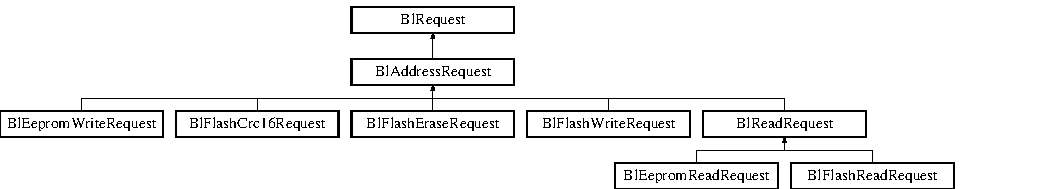
\includegraphics[height=2.539683cm]{struct_bl_address_request}
\end{center}
\end{figure}
\subsection*{Public Member Functions}
\begin{DoxyCompactItemize}
\item 
\hypertarget{struct_bl_address_request_aff4bb182ecbd0b573d424db09b9516f2}{{\bfseries Bl\-Address\-Request} (size\-\_\-t size, unsigned char cmd)}\label{struct_bl_address_request_aff4bb182ecbd0b573d424db09b9516f2}

\item 
\hypertarget{struct_bl_address_request_add81e2ca67af34bf1c94e175a57656bf}{virtual void {\bfseries Set\-Address} (unsigned int address)}\label{struct_bl_address_request_add81e2ca67af34bf1c94e175a57656bf}

\end{DoxyCompactItemize}
\subsection*{Public Attributes}
\begin{DoxyCompactItemize}
\item 
\hypertarget{struct_bl_address_request_ae6a252f564542600cecd8c370ff25955}{unsigned char {\bfseries address\-Low}}\label{struct_bl_address_request_ae6a252f564542600cecd8c370ff25955}

\item 
\hypertarget{struct_bl_address_request_a9e30628b0954a18ed75ce920a33d72ee}{unsigned char {\bfseries address\-High}}\label{struct_bl_address_request_a9e30628b0954a18ed75ce920a33d72ee}

\item 
\hypertarget{struct_bl_address_request_afd1d17701a5905becce00ef6c0a0dbd0}{unsigned char {\bfseries address\-U}}\label{struct_bl_address_request_afd1d17701a5905becce00ef6c0a0dbd0}

\item 
\hypertarget{struct_bl_address_request_a04df4477476757417bfbd0b2b5a30a19}{const unsigned char {\bfseries zero}}\label{struct_bl_address_request_a04df4477476757417bfbd0b2b5a30a19}

\end{DoxyCompactItemize}


The documentation for this struct was generated from the following file\-:\begin{DoxyCompactItemize}
\item 
library/Bl\-Request.\-h\end{DoxyCompactItemize}

\hypertarget{struct_bl_eeprom_read_request}{\section{Bl\-Eeprom\-Read\-Request Struct Reference}
\label{struct_bl_eeprom_read_request}\index{Bl\-Eeprom\-Read\-Request@{Bl\-Eeprom\-Read\-Request}}
}
Inheritance diagram for Bl\-Eeprom\-Read\-Request\-:\begin{figure}[H]
\begin{center}
\leavevmode
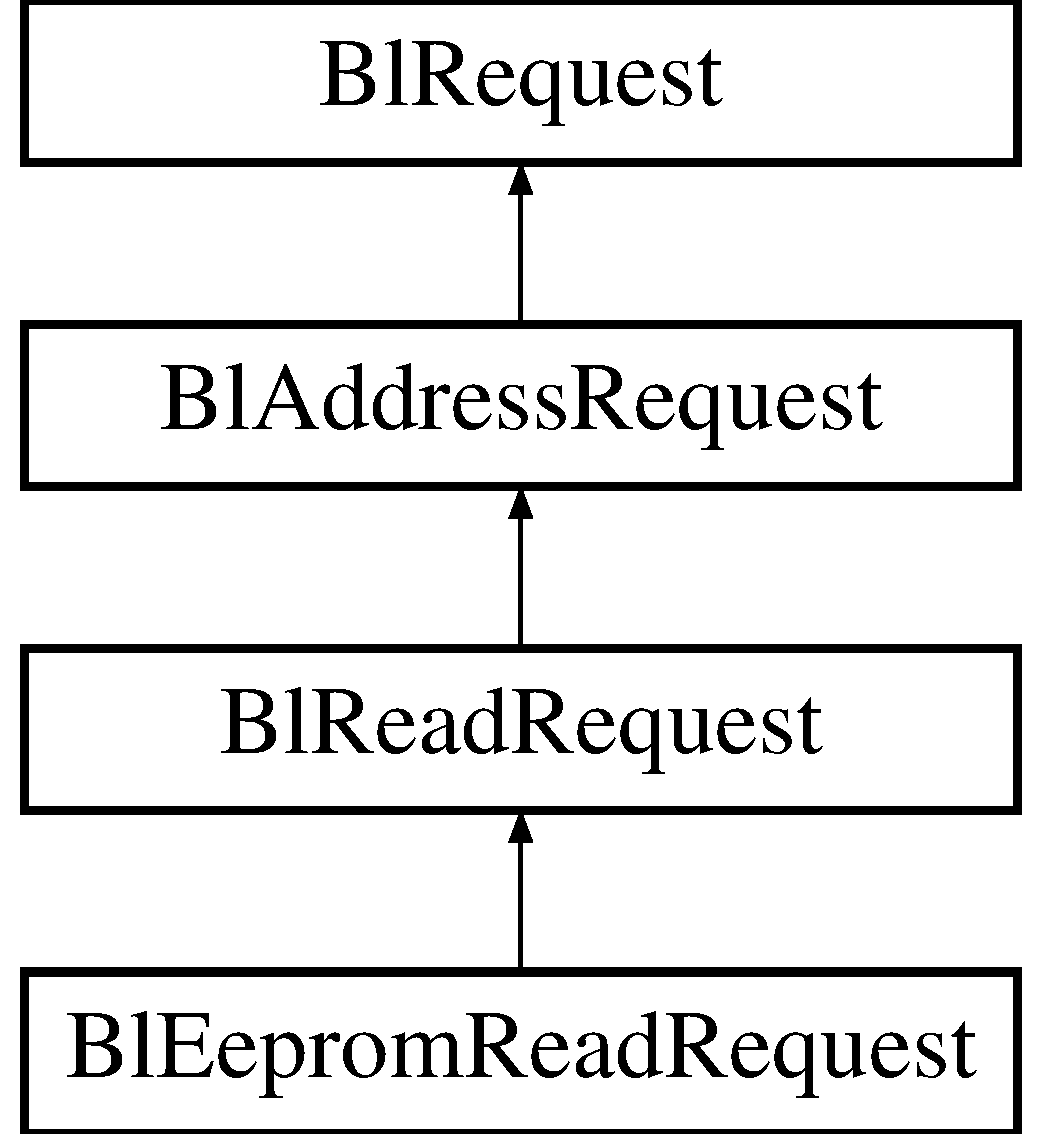
\includegraphics[height=4.000000cm]{struct_bl_eeprom_read_request}
\end{center}
\end{figure}
\subsection*{Additional Inherited Members}


The documentation for this struct was generated from the following file\-:\begin{DoxyCompactItemize}
\item 
library/Bl\-Request.\-h\end{DoxyCompactItemize}

\hypertarget{struct_bl_eeprom_write_request}{\section{Bl\-Eeprom\-Write\-Request Struct Reference}
\label{struct_bl_eeprom_write_request}\index{Bl\-Eeprom\-Write\-Request@{Bl\-Eeprom\-Write\-Request}}
}
Inheritance diagram for Bl\-Eeprom\-Write\-Request\-:\begin{figure}[H]
\begin{center}
\leavevmode
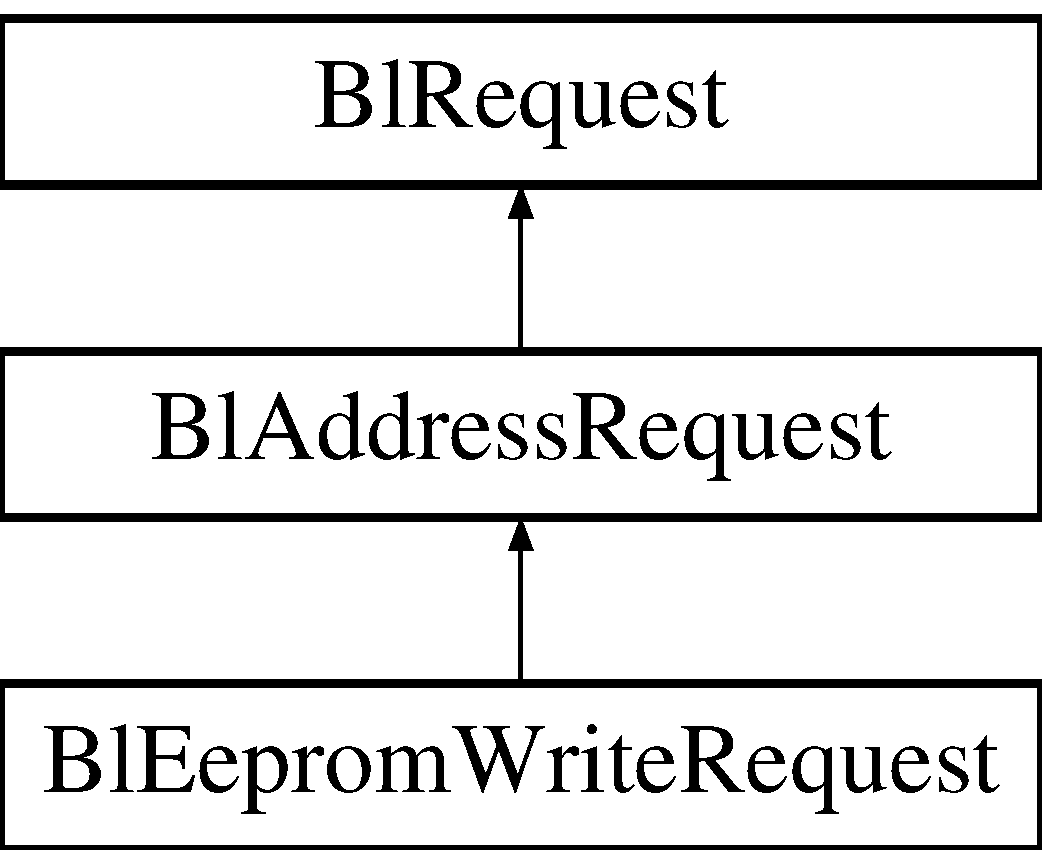
\includegraphics[height=3.000000cm]{struct_bl_eeprom_write_request}
\end{center}
\end{figure}
\subsection*{Public Member Functions}
\begin{DoxyCompactItemize}
\item 
\hypertarget{struct_bl_eeprom_write_request_afbd5e65c2c49791b2812d965fea7ca51}{void {\bfseries Set\-Data} (unsigned int address, unsigned char $\ast$p\-Data, size\-\_\-t num\-Bytes)}\label{struct_bl_eeprom_write_request_afbd5e65c2c49791b2812d965fea7ca51}

\end{DoxyCompactItemize}
\subsection*{Public Attributes}
\begin{DoxyCompactItemize}
\item 
\hypertarget{struct_bl_eeprom_write_request_a99a5d20f83d1fac437f3f54703d40e14}{unsigned char {\bfseries num\-Bytes\-Low}}\label{struct_bl_eeprom_write_request_a99a5d20f83d1fac437f3f54703d40e14}

\item 
\hypertarget{struct_bl_eeprom_write_request_ab048ccd01058cf6713bd40b7120f9584}{unsigned char {\bfseries num\-Bytes\-High}}\label{struct_bl_eeprom_write_request_ab048ccd01058cf6713bd40b7120f9584}

\item 
\hypertarget{struct_bl_eeprom_write_request_a55b1312edf28cfa81d1ca266c986ad72}{unsigned char {\bfseries payload} \mbox{[}E\-E\-P\-R\-O\-M\-\_\-\-W\-R\-I\-T\-E\-\_\-\-B\-L\-O\-C\-K\-S\-I\-Z\-E\mbox{]}}\label{struct_bl_eeprom_write_request_a55b1312edf28cfa81d1ca266c986ad72}

\end{DoxyCompactItemize}


The documentation for this struct was generated from the following file\-:\begin{DoxyCompactItemize}
\item 
library/Bl\-Request.\-h\end{DoxyCompactItemize}

\hypertarget{struct_bl_flash_crc16_request}{\section{Bl\-Flash\-Crc16\-Request Struct Reference}
\label{struct_bl_flash_crc16_request}\index{Bl\-Flash\-Crc16\-Request@{Bl\-Flash\-Crc16\-Request}}
}
Inheritance diagram for Bl\-Flash\-Crc16\-Request\-:\begin{figure}[H]
\begin{center}
\leavevmode
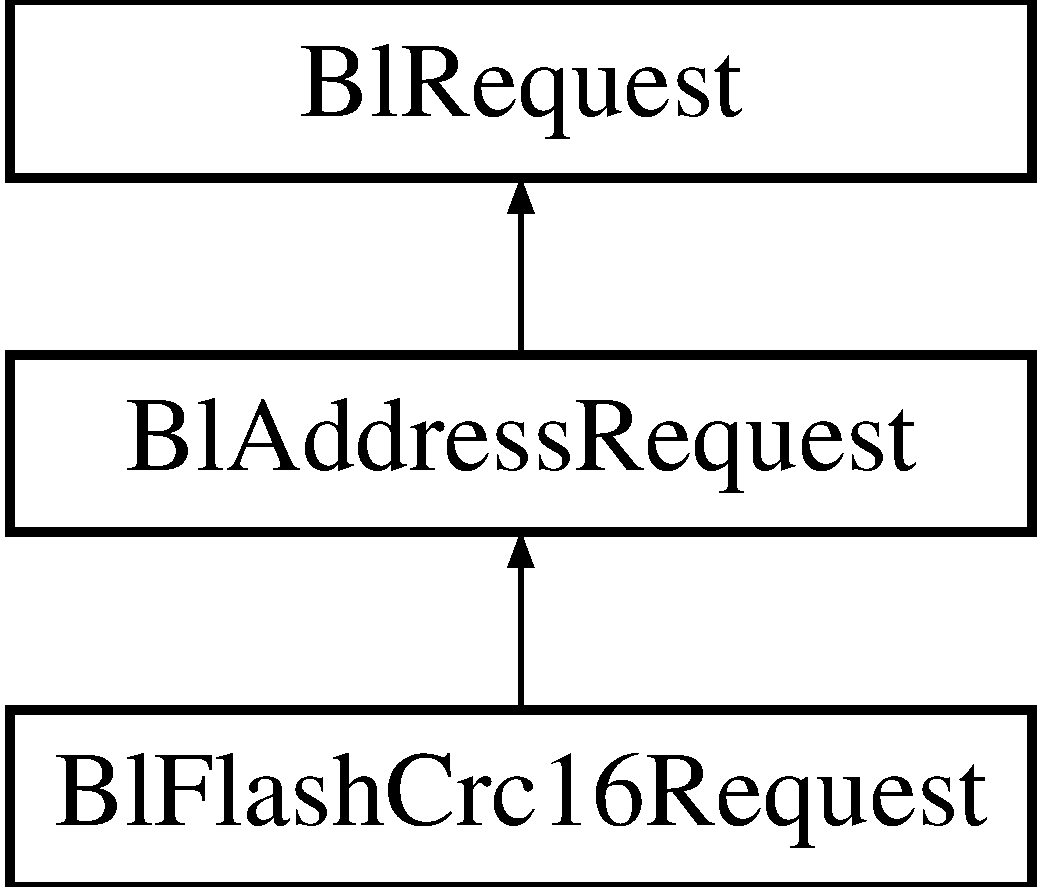
\includegraphics[height=3.000000cm]{struct_bl_flash_crc16_request}
\end{center}
\end{figure}
\subsection*{Public Member Functions}
\begin{DoxyCompactItemize}
\item 
\hypertarget{struct_bl_flash_crc16_request_a19119cb8b72cd5892ee4c75d8187ce36}{{\bfseries Bl\-Flash\-Crc16\-Request} (uint32\-\_\-t address, uint16\-\_\-t num\-Blocks)}\label{struct_bl_flash_crc16_request_a19119cb8b72cd5892ee4c75d8187ce36}

\item 
\hypertarget{struct_bl_flash_crc16_request_a8758fc8e47673ffc02fd7b79596b21d9}{virtual bool {\bfseries Check\-Crc} () const }\label{struct_bl_flash_crc16_request_a8758fc8e47673ffc02fd7b79596b21d9}

\end{DoxyCompactItemize}
\subsection*{Public Attributes}
\begin{DoxyCompactItemize}
\item 
\hypertarget{struct_bl_flash_crc16_request_a9bf380a0e7aae6cb05f382c7dbf0f659}{uint8\-\_\-t {\bfseries num\-Blocks\-Low}}\label{struct_bl_flash_crc16_request_a9bf380a0e7aae6cb05f382c7dbf0f659}

\item 
\hypertarget{struct_bl_flash_crc16_request_a99771cedf57ffdd7a1933caad05c56b8}{uint8\-\_\-t {\bfseries num\-Blocks\-High}}\label{struct_bl_flash_crc16_request_a99771cedf57ffdd7a1933caad05c56b8}

\end{DoxyCompactItemize}


The documentation for this struct was generated from the following file\-:\begin{DoxyCompactItemize}
\item 
library/Bl\-Request.\-h\end{DoxyCompactItemize}

\hypertarget{struct_bl_flash_erase_request}{\section{Bl\-Flash\-Erase\-Request Struct Reference}
\label{struct_bl_flash_erase_request}\index{Bl\-Flash\-Erase\-Request@{Bl\-Flash\-Erase\-Request}}
}
Inheritance diagram for Bl\-Flash\-Erase\-Request\-:\begin{figure}[H]
\begin{center}
\leavevmode
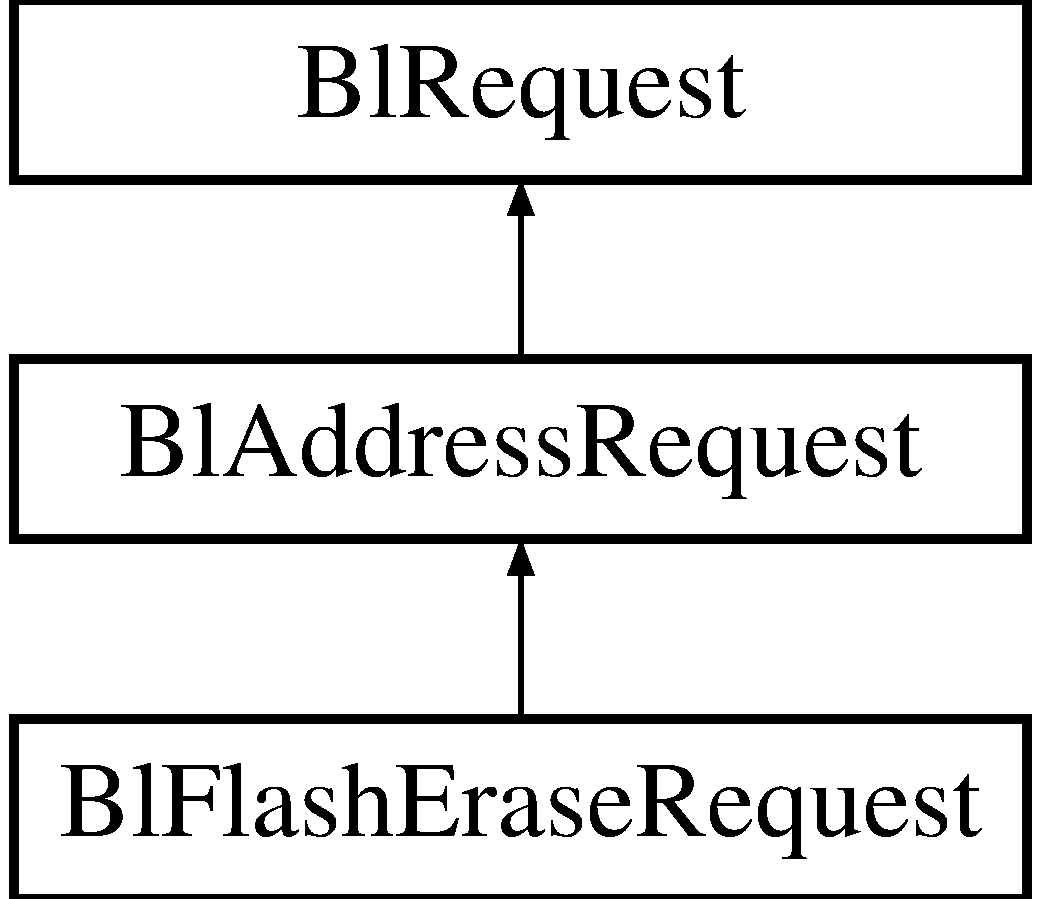
\includegraphics[height=3.000000cm]{struct_bl_flash_erase_request}
\end{center}
\end{figure}
\subsection*{Public Member Functions}
\begin{DoxyCompactItemize}
\item 
\hypertarget{struct_bl_flash_erase_request_aea945f360bd7e53e625a9235071599d8}{{\bfseries Bl\-Flash\-Erase\-Request} (uint32\-\_\-t address, uint8\-\_\-t num\-Flash\-Pages)}\label{struct_bl_flash_erase_request_aea945f360bd7e53e625a9235071599d8}

\end{DoxyCompactItemize}
\subsection*{Public Attributes}
\begin{DoxyCompactItemize}
\item 
\hypertarget{struct_bl_flash_erase_request_aa7440aea6fb9fa10b4685195b8d6f433}{const unsigned char {\bfseries num\-Pages}}\label{struct_bl_flash_erase_request_aa7440aea6fb9fa10b4685195b8d6f433}

\end{DoxyCompactItemize}


The documentation for this struct was generated from the following file\-:\begin{DoxyCompactItemize}
\item 
library/Bl\-Request.\-h\end{DoxyCompactItemize}

\hypertarget{struct_bl_flash_read_request}{\section{Bl\-Flash\-Read\-Request Struct Reference}
\label{struct_bl_flash_read_request}\index{Bl\-Flash\-Read\-Request@{Bl\-Flash\-Read\-Request}}
}
Inheritance diagram for Bl\-Flash\-Read\-Request\-:\begin{figure}[H]
\begin{center}
\leavevmode
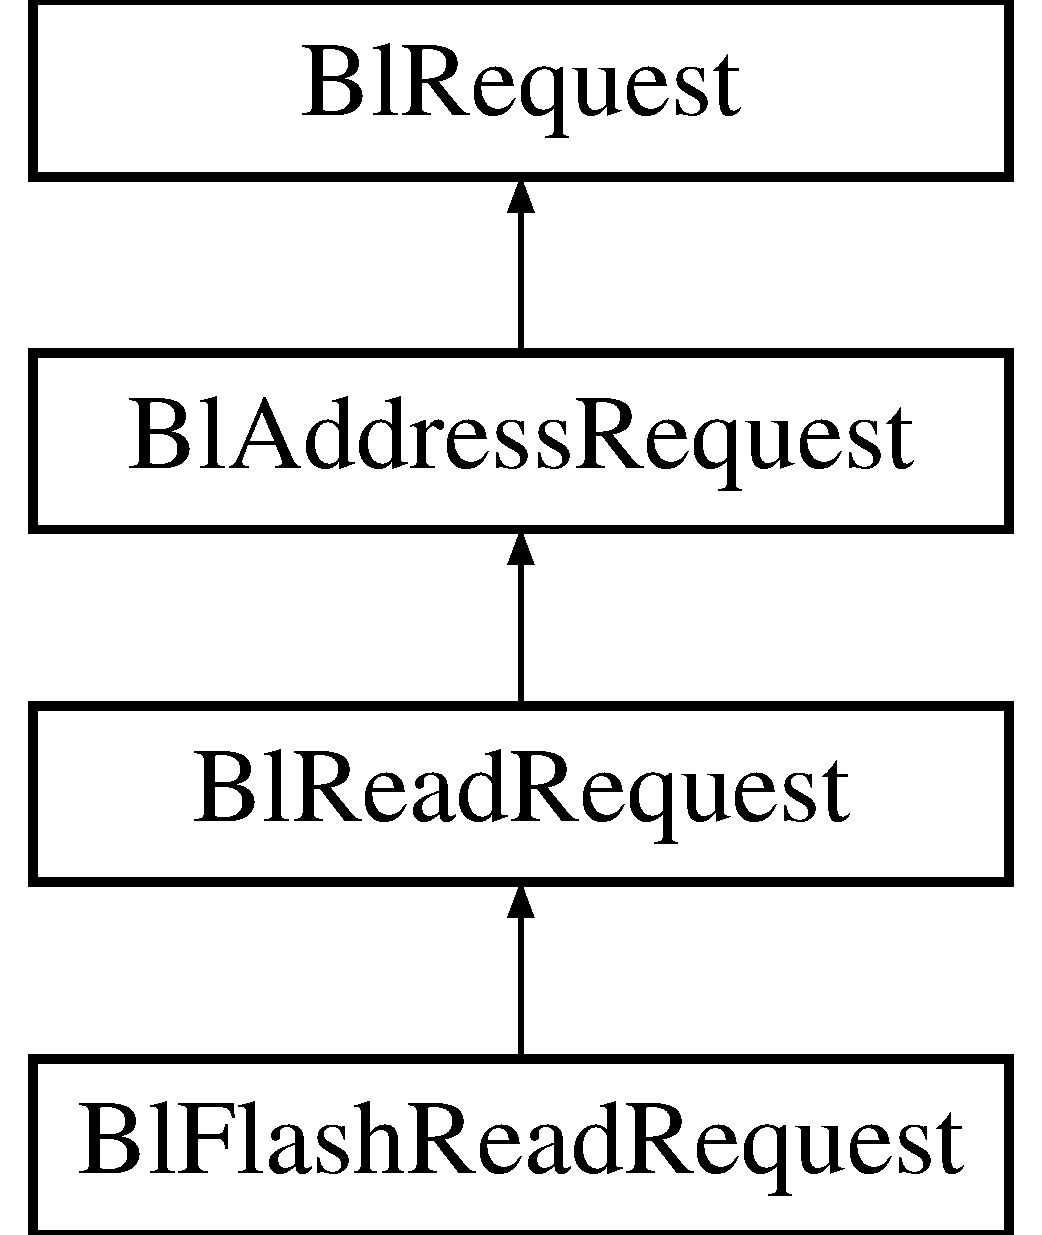
\includegraphics[height=4.000000cm]{struct_bl_flash_read_request}
\end{center}
\end{figure}
\subsection*{Additional Inherited Members}


The documentation for this struct was generated from the following file\-:\begin{DoxyCompactItemize}
\item 
library/Bl\-Request.\-h\end{DoxyCompactItemize}

\hypertarget{struct_bl_flash_write_request}{\section{Bl\-Flash\-Write\-Request Struct Reference}
\label{struct_bl_flash_write_request}\index{Bl\-Flash\-Write\-Request@{Bl\-Flash\-Write\-Request}}
}
Inheritance diagram for Bl\-Flash\-Write\-Request\-:\begin{figure}[H]
\begin{center}
\leavevmode
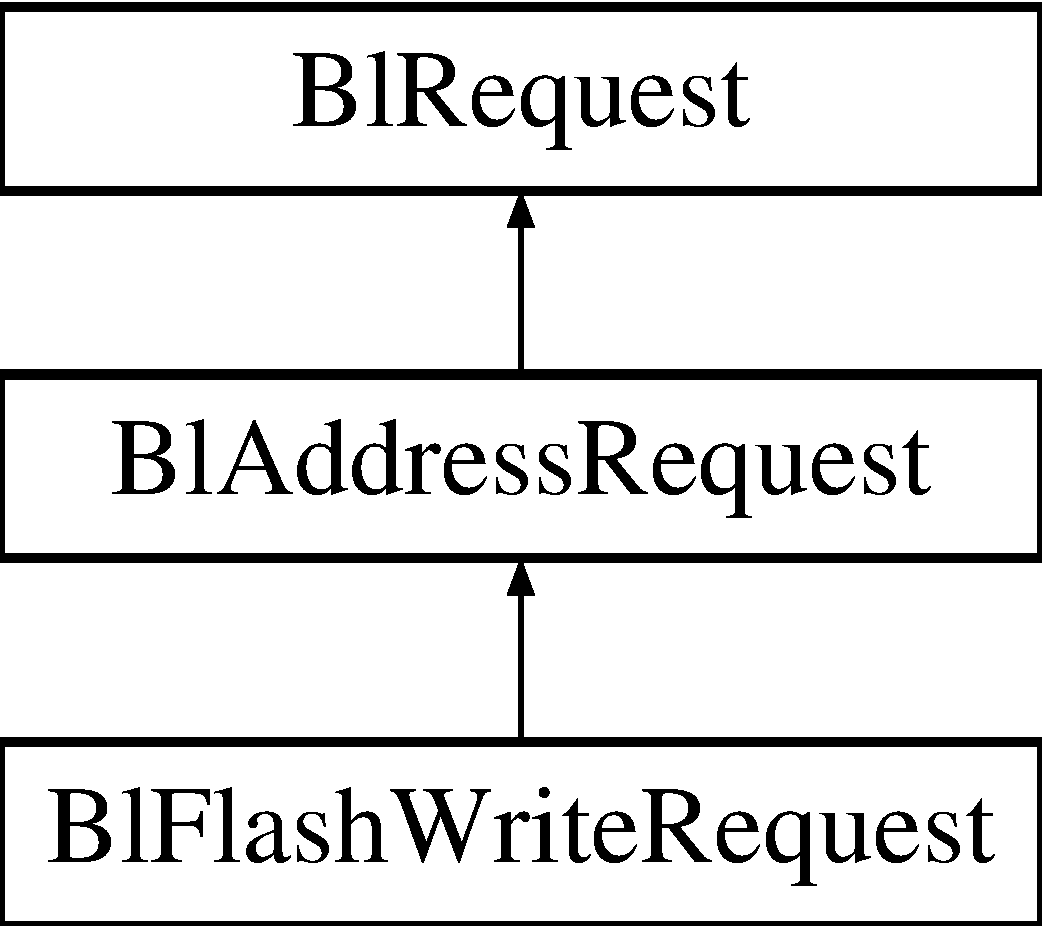
\includegraphics[height=3.000000cm]{struct_bl_flash_write_request}
\end{center}
\end{figure}
\subsection*{Public Member Functions}
\begin{DoxyCompactItemize}
\item 
\hypertarget{struct_bl_flash_write_request_acf26fc08c3d7fe8d36cc195faee09ac8}{void {\bfseries Set\-Data} (unsigned int address, unsigned char $\ast$p\-Data, size\-\_\-t num\-Bytes)}\label{struct_bl_flash_write_request_acf26fc08c3d7fe8d36cc195faee09ac8}

\end{DoxyCompactItemize}
\subsection*{Public Attributes}
\begin{DoxyCompactItemize}
\item 
\hypertarget{struct_bl_flash_write_request_abff06b9442ac201c7bfb163705c90cf5}{unsigned char {\bfseries num\-Blocks\-Low}}\label{struct_bl_flash_write_request_abff06b9442ac201c7bfb163705c90cf5}

\item 
\hypertarget{struct_bl_flash_write_request_af4981efac8d54dcf31f7666f22df17f5}{unsigned char {\bfseries payload} \mbox{[}F\-L\-A\-S\-H\-\_\-\-W\-R\-I\-T\-E\-\_\-\-B\-L\-O\-C\-K\-S\-I\-Z\-E\mbox{]}}\label{struct_bl_flash_write_request_af4981efac8d54dcf31f7666f22df17f5}

\end{DoxyCompactItemize}


The documentation for this struct was generated from the following file\-:\begin{DoxyCompactItemize}
\item 
library/Bl\-Request.\-h\end{DoxyCompactItemize}

\hypertarget{struct_bl_info}{\section{Bl\-Info Struct Reference}
\label{struct_bl_info}\index{Bl\-Info@{Bl\-Info}}
}
\subsection*{Public Member Functions}
\begin{DoxyCompactItemize}
\item 
\hypertarget{struct_bl_info_a54a7c7a8982f9ed99517977a9089da62}{uint32\-\_\-t {\bfseries Get\-Address} (void) const }\label{struct_bl_info_a54a7c7a8982f9ed99517977a9089da62}

\item 
\hypertarget{struct_bl_info_a4deedea65fec600c73ad4097659a4cfa}{void {\bfseries Print} (void) const }\label{struct_bl_info_a4deedea65fec600c73ad4097659a4cfa}

\end{DoxyCompactItemize}
\subsection*{Public Attributes}
\begin{DoxyCompactItemize}
\item 
\hypertarget{struct_bl_info_af53fd31e97f796089198cf77681ba9cb}{unsigned char {\bfseries size\-Low}}\label{struct_bl_info_af53fd31e97f796089198cf77681ba9cb}

\item 
\hypertarget{struct_bl_info_a17fd7e3d13075c98cb3589a5670eaa27}{unsigned char {\bfseries size\-High}}\label{struct_bl_info_a17fd7e3d13075c98cb3589a5670eaa27}

\item 
\hypertarget{struct_bl_info_adecf35498759a50f70cfd720930c2fee}{unsigned char {\bfseries version\-Major}}\label{struct_bl_info_adecf35498759a50f70cfd720930c2fee}

\item 
\hypertarget{struct_bl_info_a013455b390e6a994503fc913ef4962ec}{unsigned char {\bfseries version\-Minor}}\label{struct_bl_info_a013455b390e6a994503fc913ef4962ec}

\item 
\hypertarget{struct_bl_info_a6230bfa0bbba06b6d4cbf4a091f29206}{unsigned char {\bfseries cmdmask\-High}}\label{struct_bl_info_a6230bfa0bbba06b6d4cbf4a091f29206}

\item 
\hypertarget{struct_bl_info_aa83c1399c74fbc43483497e25d01a944}{unsigned char {\bfseries family\-Id}\-: 4}\label{struct_bl_info_aa83c1399c74fbc43483497e25d01a944}

\item 
\hypertarget{struct_bl_info_a1f12826be55d13f19c756bc5e3428b3c}{unsigned char {\bfseries cmdmask\-Low}\-:4}\label{struct_bl_info_a1f12826be55d13f19c756bc5e3428b3c}

\item 
\hypertarget{struct_bl_info_a4d08750ac1951abfae43f350f11e6e74}{unsigned char {\bfseries start\-Low}}\label{struct_bl_info_a4d08750ac1951abfae43f350f11e6e74}

\item 
\hypertarget{struct_bl_info_a952bed33ae2583318cb548e5af1ee0f7}{unsigned char {\bfseries start\-High}}\label{struct_bl_info_a952bed33ae2583318cb548e5af1ee0f7}

\item 
\hypertarget{struct_bl_info_ad0ff495d980e4852f048e4b8f3f937aa}{unsigned char {\bfseries start\-U}}\label{struct_bl_info_ad0ff495d980e4852f048e4b8f3f937aa}

\item 
\hypertarget{struct_bl_info_a46dfaab15225f0149142be16b0976216}{unsigned char {\bfseries zero}}\label{struct_bl_info_a46dfaab15225f0149142be16b0976216}

\end{DoxyCompactItemize}


The documentation for this struct was generated from the following file\-:\begin{DoxyCompactItemize}
\item 
library/Bl\-Request.\-h\end{DoxyCompactItemize}

\hypertarget{struct_bl_info_request}{\section{Bl\-Info\-Request Struct Reference}
\label{struct_bl_info_request}\index{Bl\-Info\-Request@{Bl\-Info\-Request}}
}
Inheritance diagram for Bl\-Info\-Request\-:\begin{figure}[H]
\begin{center}
\leavevmode
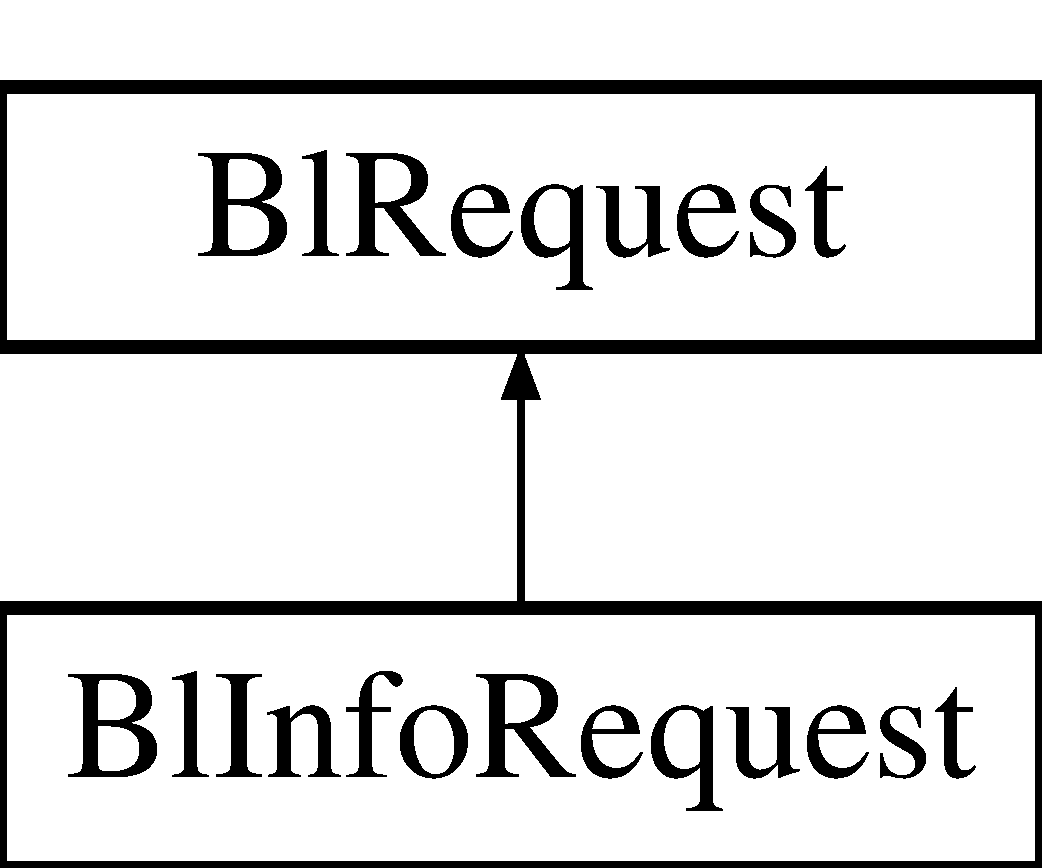
\includegraphics[height=2.000000cm]{struct_bl_info_request}
\end{center}
\end{figure}
\subsection*{Additional Inherited Members}


The documentation for this struct was generated from the following file\-:\begin{DoxyCompactItemize}
\item 
library/Bl\-Request.\-h\end{DoxyCompactItemize}

\hypertarget{class_bl_no_response_exception}{\section{Bl\-No\-Response\-Exception Class Reference}
\label{class_bl_no_response_exception}\index{Bl\-No\-Response\-Exception@{Bl\-No\-Response\-Exception}}
}
Inheritance diagram for Bl\-No\-Response\-Exception\-:\begin{figure}[H]
\begin{center}
\leavevmode
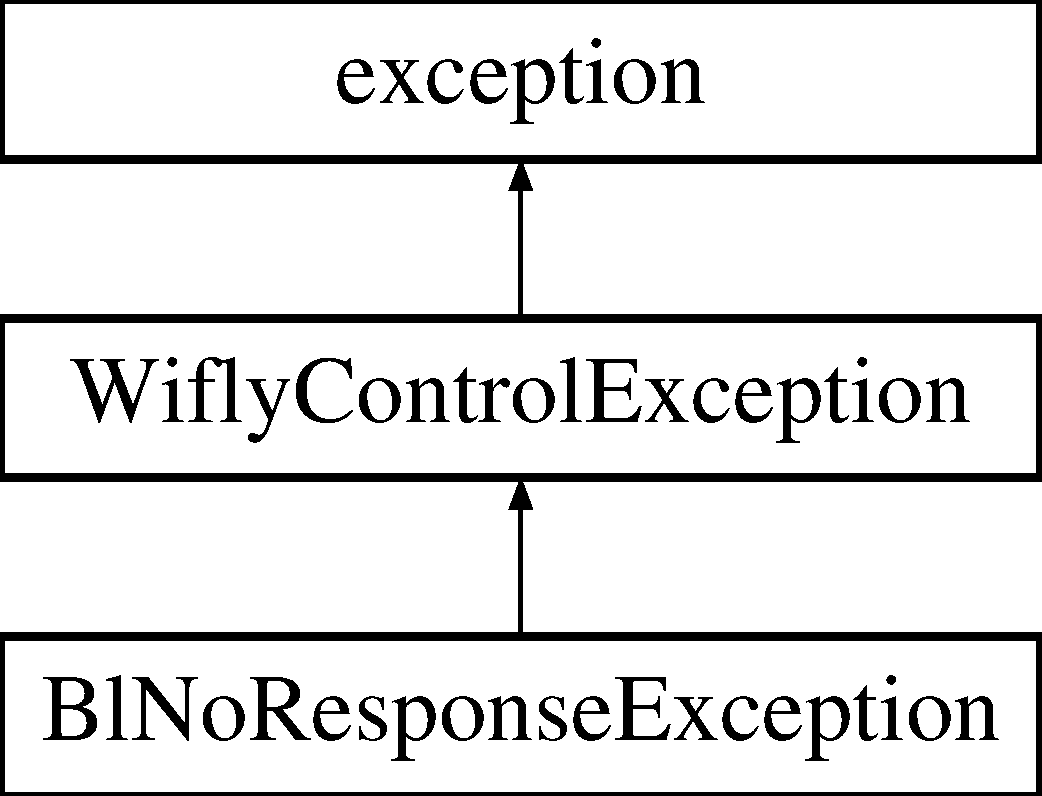
\includegraphics[height=3.000000cm]{class_bl_no_response_exception}
\end{center}
\end{figure}
\subsection*{Public Member Functions}
\begin{DoxyCompactItemize}
\item 
\hypertarget{class_bl_no_response_exception_ae3e31d1bd98466bcb7af228d1195da2c}{{\bfseries Bl\-No\-Response\-Exception} (const struct \hyperlink{struct_bl_request}{Bl\-Request} failed\-Request, const std\-::string error\-String=\char`\"{}No response received\char`\"{})}\label{class_bl_no_response_exception_ae3e31d1bd98466bcb7af228d1195da2c}

\item 
\hypertarget{class_bl_no_response_exception_aa8c6c0a7ac0e88cda1f6b04932373f5d}{struct \hyperlink{struct_bl_request}{Bl\-Request} \& {\bfseries Get\-Failed\-Request} (void) const }\label{class_bl_no_response_exception_aa8c6c0a7ac0e88cda1f6b04932373f5d}

\end{DoxyCompactItemize}


The documentation for this class was generated from the following file\-:\begin{DoxyCompactItemize}
\item 
library/Wifly\-Control\-Exception.\-h\end{DoxyCompactItemize}

\hypertarget{struct_bl_read_request}{\section{Bl\-Read\-Request Struct Reference}
\label{struct_bl_read_request}\index{Bl\-Read\-Request@{Bl\-Read\-Request}}
}
Inheritance diagram for Bl\-Read\-Request\-:\begin{figure}[H]
\begin{center}
\leavevmode
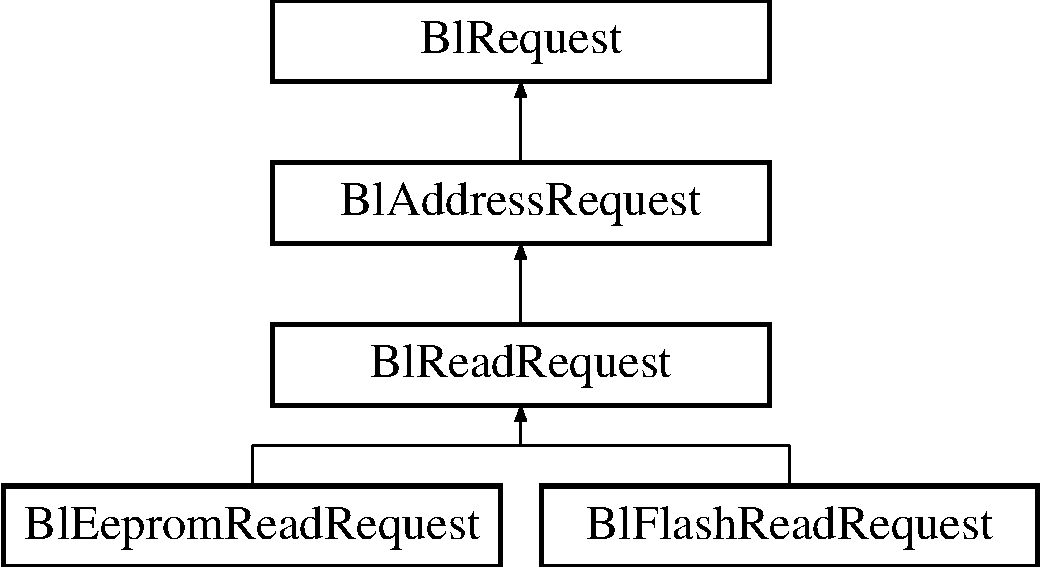
\includegraphics[height=4.000000cm]{struct_bl_read_request}
\end{center}
\end{figure}
\subsection*{Public Member Functions}
\begin{DoxyCompactItemize}
\item 
\hypertarget{struct_bl_read_request_a5e2c76a2fadad900193acedfc0f24f77}{{\bfseries Bl\-Read\-Request} (size\-\_\-t size, unsigned char cmd)}\label{struct_bl_read_request_a5e2c76a2fadad900193acedfc0f24f77}

\item 
\hypertarget{struct_bl_read_request_ad5aba1ab1c446945f62f05b21d3fac4d}{void {\bfseries Set\-Address\-Num\-Bytes} (unsigned int address, unsigned short num\-Bytes)}\label{struct_bl_read_request_ad5aba1ab1c446945f62f05b21d3fac4d}

\end{DoxyCompactItemize}
\subsection*{Public Attributes}
\begin{DoxyCompactItemize}
\item 
\hypertarget{struct_bl_read_request_a9b116d5f7400f16a396a06e15ffe7be8}{unsigned char {\bfseries num\-Bytes\-Low}}\label{struct_bl_read_request_a9b116d5f7400f16a396a06e15ffe7be8}

\item 
\hypertarget{struct_bl_read_request_a44457a87186ed4e9771c14f6751623f8}{unsigned char {\bfseries num\-Bytes\-High}}\label{struct_bl_read_request_a44457a87186ed4e9771c14f6751623f8}

\end{DoxyCompactItemize}


The documentation for this struct was generated from the following file\-:\begin{DoxyCompactItemize}
\item 
library/Bl\-Request.\-h\end{DoxyCompactItemize}

\hypertarget{struct_bl_request}{\section{Bl\-Request Struct Reference}
\label{struct_bl_request}\index{Bl\-Request@{Bl\-Request}}
}
Inheritance diagram for Bl\-Request\-:\begin{figure}[H]
\begin{center}
\leavevmode
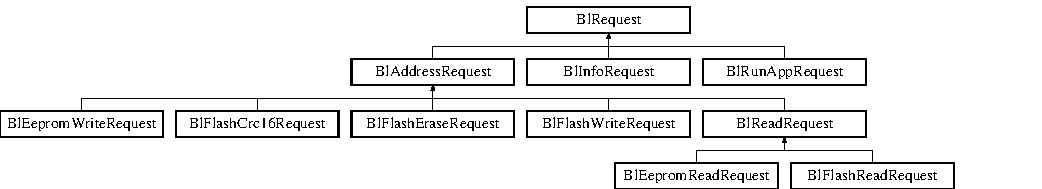
\includegraphics[height=2.539683cm]{struct_bl_request}
\end{center}
\end{figure}
\subsection*{Public Member Functions}
\begin{DoxyCompactItemize}
\item 
\hypertarget{struct_bl_request_a3b8671171980b783d25f8491e55e1a58}{{\bfseries Bl\-Request} (size\-\_\-t size, unsigned char cmd)}\label{struct_bl_request_a3b8671171980b783d25f8491e55e1a58}

\item 
\hypertarget{struct_bl_request_aa96361ac208e80204a36870f79f90a83}{const unsigned char $\ast$ {\bfseries Get\-Data} () const }\label{struct_bl_request_aa96361ac208e80204a36870f79f90a83}

\item 
\hypertarget{struct_bl_request_aaf1d5f14893458a504180196837dcca3}{size\-\_\-t {\bfseries Get\-Size} () const }\label{struct_bl_request_aaf1d5f14893458a504180196837dcca3}

\item 
\hypertarget{struct_bl_request_a15810e2347a8b2170030f0c2f98fe4d8}{virtual bool {\bfseries Check\-Crc} () const }\label{struct_bl_request_a15810e2347a8b2170030f0c2f98fe4d8}

\end{DoxyCompactItemize}
\subsection*{Public Attributes}
\begin{DoxyCompactItemize}
\item 
\hypertarget{struct_bl_request_afd0174f556d9d4538de850260e8d08a4}{const size\-\_\-t {\bfseries m\-Size}}\label{struct_bl_request_afd0174f556d9d4538de850260e8d08a4}

\item 
\hypertarget{struct_bl_request_a96c808cdbb7f02eeffcea7ebcdb98d0b}{const unsigned char {\bfseries m\-Cmd}}\label{struct_bl_request_a96c808cdbb7f02eeffcea7ebcdb98d0b}

\end{DoxyCompactItemize}


The documentation for this struct was generated from the following file\-:\begin{DoxyCompactItemize}
\item 
library/Bl\-Request.\-h\end{DoxyCompactItemize}

\hypertarget{struct_bl_run_app_request}{\section{Bl\-Run\-App\-Request Struct Reference}
\label{struct_bl_run_app_request}\index{Bl\-Run\-App\-Request@{Bl\-Run\-App\-Request}}
}
Inheritance diagram for Bl\-Run\-App\-Request\-:\begin{figure}[H]
\begin{center}
\leavevmode
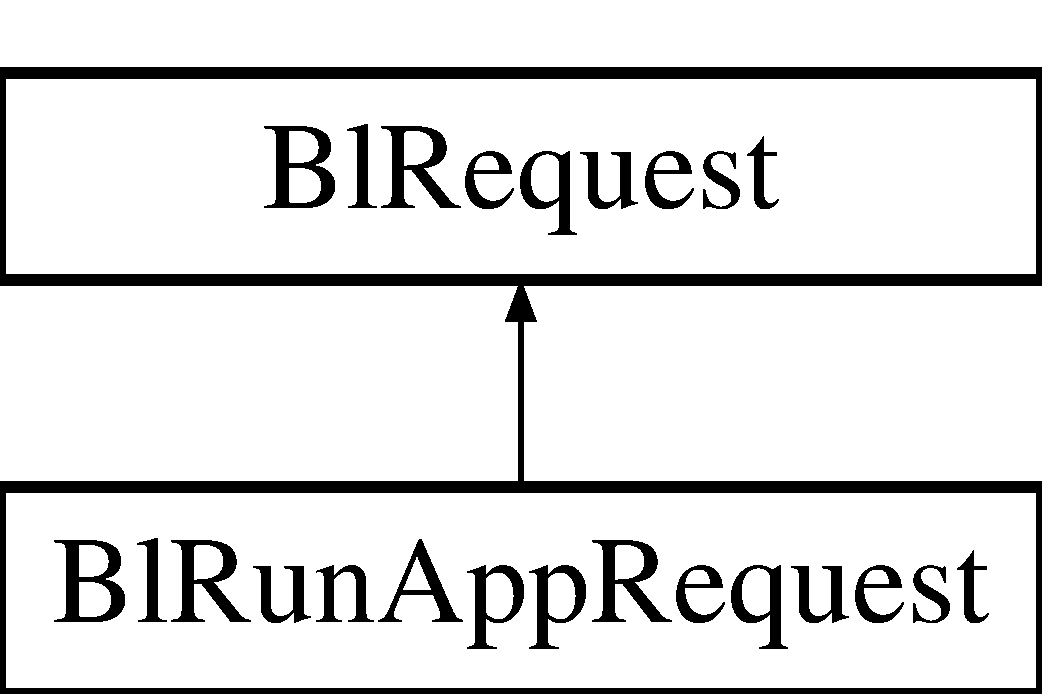
\includegraphics[height=2.000000cm]{struct_bl_run_app_request}
\end{center}
\end{figure}
\subsection*{Public Member Functions}
\begin{DoxyCompactItemize}
\item 
\hypertarget{struct_bl_run_app_request_a63e276cbe52c1aa8a3c5ec3a16e6e21b}{virtual bool {\bfseries Check\-Crc} () const }\label{struct_bl_run_app_request_a63e276cbe52c1aa8a3c5ec3a16e6e21b}

\end{DoxyCompactItemize}
\subsection*{Additional Inherited Members}


The documentation for this struct was generated from the following file\-:\begin{DoxyCompactItemize}
\item 
library/Bl\-Request.\-h\end{DoxyCompactItemize}

\hypertarget{struct_broadcast_message}{\section{Broadcast\-Message Struct Reference}
\label{struct_broadcast_message}\index{Broadcast\-Message@{Broadcast\-Message}}
}
\subsection*{Public Member Functions}
\begin{DoxyCompactItemize}
\item 
\hypertarget{struct_broadcast_message_a3050a0c141e0bd6d5333f9c7d880842c}{bool {\bfseries Is\-Wifly\-Broadcast} (size\-\_\-t length) const }\label{struct_broadcast_message_a3050a0c141e0bd6d5333f9c7d880842c}

\item 
\hypertarget{struct_broadcast_message_a73ac6b220ef0ffca03cd470ebae1e4ff}{bool {\bfseries Is\-Stop} (size\-\_\-t length) const }\label{struct_broadcast_message_a73ac6b220ef0ffca03cd470ebae1e4ff}

\end{DoxyCompactItemize}
\subsection*{Public Attributes}
\begin{DoxyCompactItemize}
\item 
\hypertarget{struct_broadcast_message_a3ac273d4896e7a2f61bc9e5e462b7f12}{uint8\-\_\-t {\bfseries mac} \mbox{[}6\mbox{]}}\label{struct_broadcast_message_a3ac273d4896e7a2f61bc9e5e462b7f12}

\item 
\hypertarget{struct_broadcast_message_a2a8000548cf6f0765d8d5a95346819e3}{uint8\-\_\-t {\bfseries channel}}\label{struct_broadcast_message_a2a8000548cf6f0765d8d5a95346819e3}

\item 
\hypertarget{struct_broadcast_message_ad01e36acd26ba12f61cf46f116173680}{uint8\-\_\-t {\bfseries rssi}}\label{struct_broadcast_message_ad01e36acd26ba12f61cf46f116173680}

\item 
\hypertarget{struct_broadcast_message_ad1b068a0ec74e5ffdb2dd0d4ab550616}{uint16\-\_\-t {\bfseries port}}\label{struct_broadcast_message_ad1b068a0ec74e5ffdb2dd0d4ab550616}

\item 
\hypertarget{struct_broadcast_message_ab7f823fa16241b8305ce51a808d534ce}{uint32\-\_\-t {\bfseries rtc}}\label{struct_broadcast_message_ab7f823fa16241b8305ce51a808d534ce}

\item 
\hypertarget{struct_broadcast_message_ad4ba25279648f3d69685a59b139c9abe}{uint16\-\_\-t {\bfseries bat\-\_\-m\-V}}\label{struct_broadcast_message_ad4ba25279648f3d69685a59b139c9abe}

\item 
\hypertarget{struct_broadcast_message_a70f920e51357cadc8b8289726cfaf9a6}{uint16\-\_\-t {\bfseries gpio\-Value}}\label{struct_broadcast_message_a70f920e51357cadc8b8289726cfaf9a6}

\item 
\hypertarget{struct_broadcast_message_aa7f6b47ac086067f235f7bf50a1ba463}{int8\-\_\-t {\bfseries ascii\-Time} \mbox{[}13+1\mbox{]}}\label{struct_broadcast_message_aa7f6b47ac086067f235f7bf50a1ba463}

\item 
\hypertarget{struct_broadcast_message_ac348f0fde101e0d4ecb2ea47de28b8dc}{int8\-\_\-t {\bfseries version} \mbox{[}26+1+1\mbox{]}}\label{struct_broadcast_message_ac348f0fde101e0d4ecb2ea47de28b8dc}

\item 
\hypertarget{struct_broadcast_message_a5eed77683f928d1454419138eed7d673}{int8\-\_\-t {\bfseries device\-Id} \mbox{[}32\mbox{]}}\label{struct_broadcast_message_a5eed77683f928d1454419138eed7d673}

\item 
\hypertarget{struct_broadcast_message_a20abccb0a47e7956cd2a3bcd3299c23c}{uint16\-\_\-t {\bfseries boot\-Tmms}}\label{struct_broadcast_message_a20abccb0a47e7956cd2a3bcd3299c23c}

\item 
\hypertarget{struct_broadcast_message_adfe11beb5dc63400e112cfe2bf59fd0b}{uint16\-\_\-t {\bfseries sensor} \mbox{[}8\mbox{]}}\label{struct_broadcast_message_adfe11beb5dc63400e112cfe2bf59fd0b}

\end{DoxyCompactItemize}


The documentation for this struct was generated from the following file\-:\begin{DoxyCompactItemize}
\item 
library/Broadcast\-Receiver.\-h\end{DoxyCompactItemize}

\hypertarget{class_broadcast_receiver}{\section{Broadcast\-Receiver Class Reference}
\label{class_broadcast_receiver}\index{Broadcast\-Receiver@{Broadcast\-Receiver}}
}


{\ttfamily \#include $<$Broadcast\-Receiver.\-h$>$}

\subsection*{Public Member Functions}
\begin{DoxyCompactItemize}
\item 
\hypertarget{class_broadcast_receiver_a9c3f8ebdef813f03edec75f88389a6ee}{{\bfseries Broadcast\-Receiver} (uint16\-\_\-t port=B\-R\-O\-A\-D\-C\-A\-S\-T\-\_\-\-P\-O\-R\-T)}\label{class_broadcast_receiver_a9c3f8ebdef813f03edec75f88389a6ee}

\item 
void \hyperlink{class_broadcast_receiver_ac2fa6c783d73121c800d3c015621964d}{operator()} (std\-::ostream \&out, timeval $\ast$timeout=N\-U\-L\-L)
\item 
\hypertarget{class_broadcast_receiver_a1c487597e1338d5e5fca55f1d89d0eb1}{const \hyperlink{class_endpoint}{Endpoint} \& {\bfseries Get\-Endpoint} (size\-\_\-t index) const }\label{class_broadcast_receiver_a1c487597e1338d5e5fca55f1d89d0eb1}

\item 
\hypertarget{class_broadcast_receiver_a4549672ea1b9b008f93b42329c8bea5f}{\hyperlink{class_endpoint}{Endpoint} {\bfseries Get\-Next\-Remote} (timeval $\ast$timeout)}\label{class_broadcast_receiver_a4549672ea1b9b008f93b42329c8bea5f}

\item 
size\-\_\-t \hyperlink{class_broadcast_receiver_a6e403e696a76c5bc8c2b9215c3d5704d}{Num\-Remotes} (void) const 
\item 
void \hyperlink{class_broadcast_receiver_ab0f0852ab37655f23bebaca888216502}{Stop} (void)
\end{DoxyCompactItemize}
\subsection*{Public Attributes}
\begin{DoxyCompactItemize}
\item 
\hypertarget{class_broadcast_receiver_a3e1de2825034cb6e2b15641c490d9381}{const uint16\-\_\-t {\bfseries m\-Port}}\label{class_broadcast_receiver_a3e1de2825034cb6e2b15641c490d9381}

\end{DoxyCompactItemize}
\subsection*{Static Public Attributes}
\begin{DoxyCompactItemize}
\item 
\hypertarget{class_broadcast_receiver_a38d37ce60dc1fb1e0dbc08d80b5d3b47}{static const uint16\-\_\-t {\bfseries B\-R\-O\-A\-D\-C\-A\-S\-T\-\_\-\-P\-O\-R\-T} = 55555}\label{class_broadcast_receiver_a38d37ce60dc1fb1e0dbc08d80b5d3b47}

\item 
\hypertarget{class_broadcast_receiver_a7314a4107fc6e1c3d8dbace2b47c07d1}{static const std\-::string {\bfseries D\-E\-V\-I\-C\-E\-\_\-\-I\-D}}\label{class_broadcast_receiver_a7314a4107fc6e1c3d8dbace2b47c07d1}

\item 
\hypertarget{class_broadcast_receiver_addb5597142e98c3c16afce397082d960}{static const std\-::string {\bfseries D\-E\-V\-I\-C\-E\-\_\-\-I\-D\-\_\-\-O\-L\-D}}\label{class_broadcast_receiver_addb5597142e98c3c16afce397082d960}

\item 
\hypertarget{class_broadcast_receiver_a8a59a09e4b750cc992d9aab3a4c06a33}{static const int8\-\_\-t {\bfseries S\-T\-O\-P\-\_\-\-M\-S\-G} \mbox{[}$\,$\mbox{]}}\label{class_broadcast_receiver_a8a59a09e4b750cc992d9aab3a4c06a33}

\item 
\hypertarget{class_broadcast_receiver_afa28d7c0a9058e830c7586e33acc6b69}{static const size\-\_\-t {\bfseries S\-T\-O\-P\-\_\-\-M\-S\-G\-\_\-\-L\-E\-N\-G\-T\-H}}\label{class_broadcast_receiver_afa28d7c0a9058e830c7586e33acc6b69}

\item 
\hypertarget{class_broadcast_receiver_a545fbd086416bfa77cd42b531d045a5b}{static const \hyperlink{class_endpoint}{Endpoint} {\bfseries E\-M\-P\-T\-Y\-\_\-\-E\-N\-D\-P\-O\-I\-N\-T}}\label{class_broadcast_receiver_a545fbd086416bfa77cd42b531d045a5b}

\end{DoxyCompactItemize}


\subsection{Detailed Description}
Copyright (C) 2012, 2013 Nils Weiss, Patrick Bruenn.

This file is part of Wifly\-\_\-\-Light.

Wifly\-\_\-\-Light is free software\-: you can redistribute it and/or modify it under the terms of the G\-N\-U General Public License as published by the Free Software Foundation, either version 3 of the License, or (at your option) any later version.

Wifly\-\_\-\-Light is distributed in the hope that it will be useful, but W\-I\-T\-H\-O\-U\-T A\-N\-Y W\-A\-R\-R\-A\-N\-T\-Y; without even the implied warranty of M\-E\-R\-C\-H\-A\-N\-T\-A\-B\-I\-L\-I\-T\-Y or F\-I\-T\-N\-E\-S\-S F\-O\-R A P\-A\-R\-T\-I\-C\-U\-L\-A\-R P\-U\-R\-P\-O\-S\-E. See the G\-N\-U General Public License for more details.

You should have received a copy of the G\-N\-U General Public License along with Wifly\-\_\-\-Light. If not, see \href{http://www.gnu.org/licenses/}{\tt http\-://www.\-gnu.\-org/licenses/}. 

\subsection{Member Function Documentation}
\hypertarget{class_broadcast_receiver_a6e403e696a76c5bc8c2b9215c3d5704d}{\index{Broadcast\-Receiver@{Broadcast\-Receiver}!Num\-Remotes@{Num\-Remotes}}
\index{Num\-Remotes@{Num\-Remotes}!BroadcastReceiver@{Broadcast\-Receiver}}
\subsubsection[{Num\-Remotes}]{\setlength{\rightskip}{0pt plus 5cm}size\-\_\-t Broadcast\-Receiver\-::\-Num\-Remotes (
\begin{DoxyParamCaption}
\item[{void}]{}
\end{DoxyParamCaption}
) const}}\label{class_broadcast_receiver_a6e403e696a76c5bc8c2b9215c3d5704d}
\begin{DoxyReturn}{Returns}
number of known I\-P addresses 
\end{DoxyReturn}
\hypertarget{class_broadcast_receiver_ac2fa6c783d73121c800d3c015621964d}{\index{Broadcast\-Receiver@{Broadcast\-Receiver}!operator()@{operator()}}
\index{operator()@{operator()}!BroadcastReceiver@{Broadcast\-Receiver}}
\subsubsection[{operator()}]{\setlength{\rightskip}{0pt plus 5cm}void Broadcast\-Receiver\-::operator() (
\begin{DoxyParamCaption}
\item[{std\-::ostream \&}]{out, }
\item[{timeval $\ast$}]{timeout = {\ttfamily NULL}}
\end{DoxyParamCaption}
)}}\label{class_broadcast_receiver_ac2fa6c783d73121c800d3c015621964d}
Wait for broadcasts and print them to a stream 
\begin{DoxyParams}{Parameters}
{\em out} & stream to print collected remotes on \\
\hline
{\em timeout} & in seconds, until execution is terminated \\
\hline
\end{DoxyParams}
\hypertarget{class_broadcast_receiver_ab0f0852ab37655f23bebaca888216502}{\index{Broadcast\-Receiver@{Broadcast\-Receiver}!Stop@{Stop}}
\index{Stop@{Stop}!BroadcastReceiver@{Broadcast\-Receiver}}
\subsubsection[{Stop}]{\setlength{\rightskip}{0pt plus 5cm}void Broadcast\-Receiver\-::\-Stop (
\begin{DoxyParamCaption}
\item[{void}]{}
\end{DoxyParamCaption}
)}}\label{class_broadcast_receiver_ab0f0852ab37655f23bebaca888216502}
Sends a stop event to terminate execution of operator() 

The documentation for this class was generated from the following file\-:\begin{DoxyCompactItemize}
\item 
library/Broadcast\-Receiver.\-h\end{DoxyCompactItemize}

\hypertarget{class_client_socket}{\section{Client\-Socket Class Reference}
\label{class_client_socket}\index{Client\-Socket@{Client\-Socket}}
}


{\ttfamily \#include $<$Client\-Socket.\-h$>$}

Inheritance diagram for Client\-Socket\-:\begin{figure}[H]
\begin{center}
\leavevmode
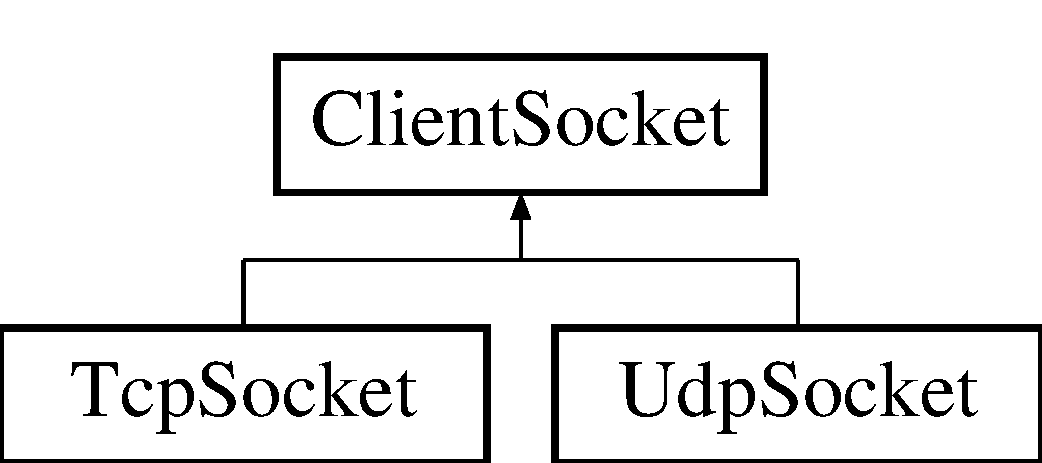
\includegraphics[height=2.000000cm]{class_client_socket}
\end{center}
\end{figure}
\subsection*{Public Member Functions}
\begin{DoxyCompactItemize}
\item 
\hypertarget{class_client_socket_a9ef0e9b489c27a59ddcc5b863d70c5c4}{{\bfseries Client\-Socket} (uint32\-\_\-t addr, uint16\-\_\-t port, int style)}\label{class_client_socket_a9ef0e9b489c27a59ddcc5b863d70c5c4}

\item 
\hypertarget{class_client_socket_ad53cfcbf3eebbfb8b8314f58d3354edd}{virtual size\-\_\-t {\bfseries Send} (const uint8\-\_\-t $\ast$frame, size\-\_\-t length) const =0}\label{class_client_socket_ad53cfcbf3eebbfb8b8314f58d3354edd}

\end{DoxyCompactItemize}
\subsection*{Protected Attributes}
\begin{DoxyCompactItemize}
\item 
\hypertarget{class_client_socket_acb5029d09ef913c0b444e97f2cc98bef}{const int {\bfseries m\-Sock}}\label{class_client_socket_acb5029d09ef913c0b444e97f2cc98bef}

\item 
\hypertarget{class_client_socket_acbf9ed9f1ebac9348a2d1c77b516acbc}{struct sockaddr\-\_\-in {\bfseries m\-Sock\-Addr}}\label{class_client_socket_acbf9ed9f1ebac9348a2d1c77b516acbc}

\end{DoxyCompactItemize}


\subsection{Detailed Description}
\begin{DoxyVerb}Copyright (C) 2012, 2013 Nils Weiss, Patrick Bruenn.
\end{DoxyVerb}


This file is part of Wifly\-\_\-\-Light.

Wifly\-\_\-\-Light is free software\-: you can redistribute it and/or modify it under the terms of the G\-N\-U General Public License as published by the Free Software Foundation, either version 3 of the License, or (at your option) any later version.

Wifly\-\_\-\-Light is distributed in the hope that it will be useful, but W\-I\-T\-H\-O\-U\-T A\-N\-Y W\-A\-R\-R\-A\-N\-T\-Y; without even the implied warranty of M\-E\-R\-C\-H\-A\-N\-T\-A\-B\-I\-L\-I\-T\-Y or F\-I\-T\-N\-E\-S\-S F\-O\-R A P\-A\-R\-T\-I\-C\-U\-L\-A\-R P\-U\-R\-P\-O\-S\-E. See the G\-N\-U General Public License for more details.

You should have received a copy of the G\-N\-U General Public License along with Wifly\-\_\-\-Light. If not, see \href{http://www.gnu.org/licenses/}{\tt http\-://www.\-gnu.\-org/licenses/}. 

The documentation for this class was generated from the following files\-:\begin{DoxyCompactItemize}
\item 
library/Client\-Socket.\-h\item 
library/Broadcast\-Receiver\-\_\-ut.\-cpp\item 
library/Client\-Socket.\-cpp\item 
library/Com\-Proxy\-\_\-ut.\-cpp\item 
library/Telnet\-Proxy\-\_\-ut.\-cpp\item 
library/Wifly\-Control\-\_\-ut.\-cpp\end{DoxyCompactItemize}

\hypertarget{class_com_proxy}{\section{Com\-Proxy Class Reference}
\label{class_com_proxy}\index{Com\-Proxy@{Com\-Proxy}}
}


{\ttfamily \#include $<$Com\-Proxy.\-h$>$}

\subsection*{Public Member Functions}
\begin{DoxyCompactItemize}
\item 
\hypertarget{class_com_proxy_a71069fbcb6901649f75f7b816559e061}{{\bfseries Com\-Proxy} (const \hyperlink{class_tcp_socket}{Tcp\-Socket} \&sock)}\label{class_com_proxy_a71069fbcb6901649f75f7b816559e061}

\item 
size\-\_\-t \hyperlink{class_com_proxy_ada3a89b37980a3e14d3f76341db0c78e}{Mask\-Control\-Characters} (const uint8\-\_\-t $\ast$p\-Input, size\-\_\-t input\-Length, uint8\-\_\-t $\ast$p\-Output, size\-\_\-t output\-Length, bool crc\-In\-Little\-Endian=true) const 
\item 
\hypertarget{class_com_proxy_a58c03dfa5d87cbad6ce77257c5195eb4}{int32\-\_\-t {\bfseries Send} (\hyperlink{struct_bl_request}{Bl\-Request} \&req, uint8\-\_\-t $\ast$p\-Response, size\-\_\-t response\-Size, bool do\-Sync=true) const }\label{class_com_proxy_a58c03dfa5d87cbad6ce77257c5195eb4}

\item 
\hypertarget{class_com_proxy_ab6205e7b4fbfcce8066e3019f5b52fb0}{int32\-\_\-t {\bfseries Send} (struct cmd\-\_\-frame const $\ast$p\-Frame, response\-\_\-frame $\ast$p\-Response, size\-\_\-t response\-Size, bool do\-Sync) const }\label{class_com_proxy_ab6205e7b4fbfcce8066e3019f5b52fb0}

\item 
\hypertarget{class_com_proxy_a5d07c1c822e4ce825236900a6b15e020}{int32\-\_\-t {\bfseries Send} (uint8\-\_\-t const $\ast$p\-Request, const size\-\_\-t request\-Size, uint8\-\_\-t $\ast$p\-Response, size\-\_\-t response\-Size, bool check\-Crc, bool sync, bool crc\-In\-Little\-Endian=true) const }\label{class_com_proxy_a5d07c1c822e4ce825236900a6b15e020}

\item 
\hypertarget{class_com_proxy_a533dbda1e24b846609c153c7545baba0}{size\-\_\-t {\bfseries Unmask\-Control\-Characters} (const uint8\-\_\-t $\ast$p\-Input, size\-\_\-t input\-Length, uint8\-\_\-t $\ast$p\-Output, size\-\_\-t output\-Length, bool check\-Crc, bool crc\-In\-Little\-Endian=true) const }\label{class_com_proxy_a533dbda1e24b846609c153c7545baba0}

\end{DoxyCompactItemize}


\subsection{Detailed Description}
Copyright (C) 2012, 2013 Nils Weiss, Patrick Bruenn.

This file is part of Wifly\-\_\-\-Light.

Wifly\-\_\-\-Light is free software\-: you can redistribute it and/or modify it under the terms of the G\-N\-U General Public License as published by the Free Software Foundation, either version 3 of the License, or (at your option) any later version.

Wifly\-\_\-\-Light is distributed in the hope that it will be useful, but W\-I\-T\-H\-O\-U\-T A\-N\-Y W\-A\-R\-R\-A\-N\-T\-Y; without even the implied warranty of M\-E\-R\-C\-H\-A\-N\-T\-A\-B\-I\-L\-I\-T\-Y or F\-I\-T\-N\-E\-S\-S F\-O\-R A P\-A\-R\-T\-I\-C\-U\-L\-A\-R P\-U\-R\-P\-O\-S\-E. See the G\-N\-U General Public License for more details.

You should have received a copy of the G\-N\-U General Public License along with Wifly\-\_\-\-Light. If not, see \href{http://www.gnu.org/licenses/}{\tt http\-://www.\-gnu.\-org/licenses/}. 

\subsection{Member Function Documentation}
\hypertarget{class_com_proxy_ada3a89b37980a3e14d3f76341db0c78e}{\index{Com\-Proxy@{Com\-Proxy}!Mask\-Control\-Characters@{Mask\-Control\-Characters}}
\index{Mask\-Control\-Characters@{Mask\-Control\-Characters}!ComProxy@{Com\-Proxy}}
\subsubsection[{Mask\-Control\-Characters}]{\setlength{\rightskip}{0pt plus 5cm}size\-\_\-t Com\-Proxy\-::\-Mask\-Control\-Characters (
\begin{DoxyParamCaption}
\item[{const uint8\-\_\-t $\ast$}]{p\-Input, }
\item[{size\-\_\-t}]{input\-Length, }
\item[{uint8\-\_\-t $\ast$}]{p\-Output, }
\item[{size\-\_\-t}]{output\-Length, }
\item[{bool}]{crc\-In\-Little\-Endian = {\ttfamily true}}
\end{DoxyParamCaption}
) const}}\label{class_com_proxy_ada3a89b37980a3e14d3f76341db0c78e}
Mask bytes of input buffer and add C\-R\-C16-\/\-C\-I\-T\-T checksum to the end 
\begin{DoxyParams}{Parameters}
{\em p\-Input} & input buffer \\
\hline
{\em input\-Length} & number of bytes in input buffer \\
\hline
{\em p\-Output} & output buffer \\
\hline
{\em output\-Length} & size of the output buffer \\
\hline
\end{DoxyParams}


The documentation for this class was generated from the following file\-:\begin{DoxyCompactItemize}
\item 
library/Com\-Proxy.\-h\end{DoxyCompactItemize}

\hypertarget{class_cycletime_response}{\section{Cycletime\-Response Class Reference}
\label{class_cycletime_response}\index{Cycletime\-Response@{Cycletime\-Response}}
}
Inheritance diagram for Cycletime\-Response\-:\begin{figure}[H]
\begin{center}
\leavevmode
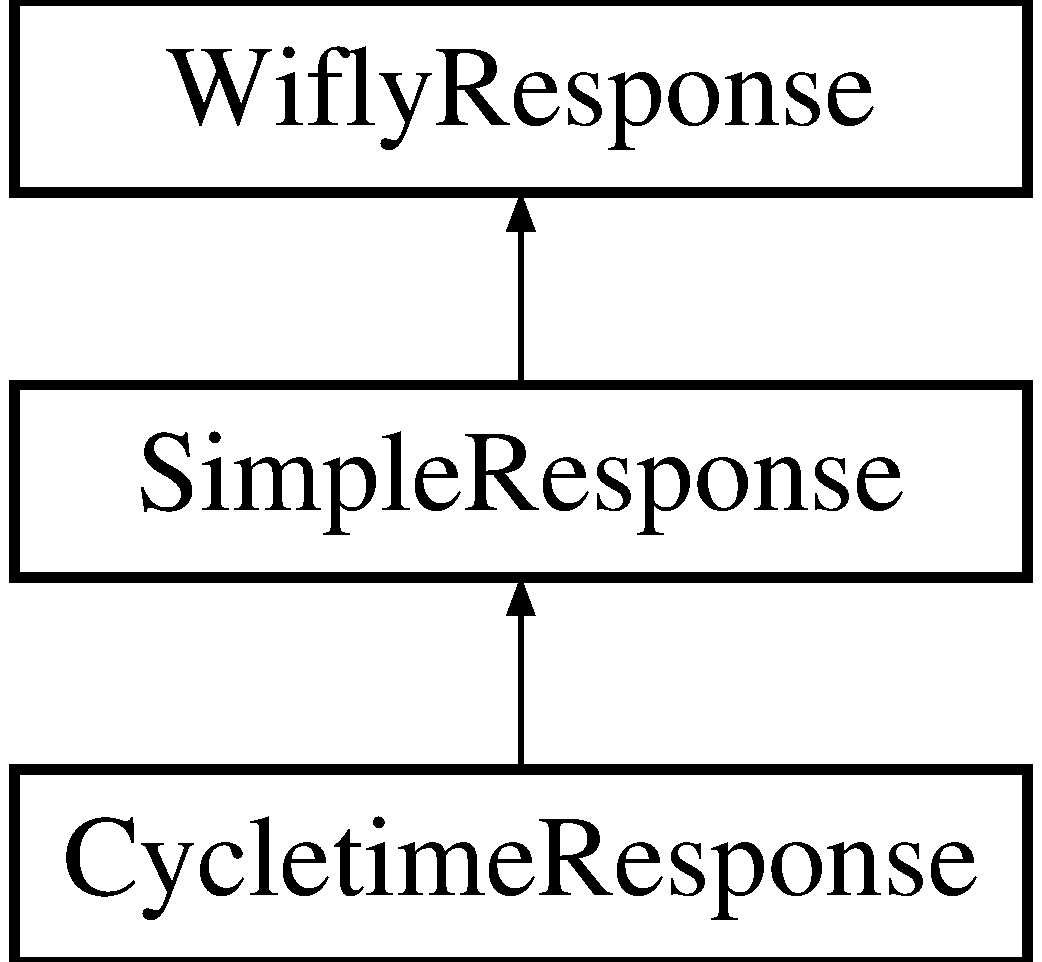
\includegraphics[height=3.000000cm]{class_cycletime_response}
\end{center}
\end{figure}
\subsection*{Public Member Functions}
\begin{DoxyCompactItemize}
\item 
\hypertarget{class_cycletime_response_ada97d2caf35ad02157828780c66bbaf4}{void {\bfseries Init} (response\-\_\-frame $\ast$p\-Data, size\-\_\-t data\-Length)}\label{class_cycletime_response_ada97d2caf35ad02157828780c66bbaf4}

\end{DoxyCompactItemize}
\subsection*{Friends}
\begin{DoxyCompactItemize}
\item 
\hypertarget{class_cycletime_response_a297451ca9509cdee481811027a5e31a6}{std\-::ostream \& {\bfseries operator$<$$<$} (std\-::ostream \&out, const \hyperlink{class_cycletime_response}{Cycletime\-Response} \&ref)}\label{class_cycletime_response_a297451ca9509cdee481811027a5e31a6}

\end{DoxyCompactItemize}
\subsection*{Additional Inherited Members}


The documentation for this class was generated from the following file\-:\begin{DoxyCompactItemize}
\item 
library/Wifly\-Control\-Response.\-h\end{DoxyCompactItemize}

\hypertarget{class_endpoint}{\section{Endpoint Class Reference}
\label{class_endpoint}\index{Endpoint@{Endpoint}}
}


{\ttfamily \#include $<$Endpoint.\-h$>$}

\subsection*{Public Member Functions}
\begin{DoxyCompactItemize}
\item 
\hypertarget{class_endpoint_a155f5e34aad88e781207ffa55666992f}{{\bfseries Endpoint} (sockaddr\-\_\-storage \&addr, const size\-\_\-t size, uint16\-\_\-t port)}\label{class_endpoint_a155f5e34aad88e781207ffa55666992f}

\item 
\hypertarget{class_endpoint_aea663fa6d602bd9b0ee36a0a20c10515}{{\bfseries Endpoint} (uint32\-\_\-t addr=0, uint16\-\_\-t port=0)}\label{class_endpoint_aea663fa6d602bd9b0ee36a0a20c10515}

\item 
\hypertarget{class_endpoint_a1ebaa89afaae9dd7b1305532634c2871}{bool {\bfseries operator$<$} (const \hyperlink{class_endpoint}{Endpoint} \&ref) const }\label{class_endpoint_a1ebaa89afaae9dd7b1305532634c2871}

\item 
\hypertarget{class_endpoint_a2d0912e7fa4ae54f9402d6833a6d3ae6}{uint64\-\_\-t {\bfseries As\-Uint64} (void) const }\label{class_endpoint_a2d0912e7fa4ae54f9402d6833a6d3ae6}

\item 
\hypertarget{class_endpoint_a5618578a2aea0258faac2ec166809f61}{uint32\-\_\-t {\bfseries Get\-Ip} (void) const }\label{class_endpoint_a5618578a2aea0258faac2ec166809f61}

\item 
\hypertarget{class_endpoint_ab314920c2ea906136bb10db9a8b19d9f}{uint16\-\_\-t {\bfseries Get\-Port} (void) const }\label{class_endpoint_ab314920c2ea906136bb10db9a8b19d9f}

\item 
\hypertarget{class_endpoint_a514014f7d1ee63a7c5a3ed7c8b129526}{bool {\bfseries Is\-Valid} (void) const }\label{class_endpoint_a514014f7d1ee63a7c5a3ed7c8b129526}

\end{DoxyCompactItemize}
\subsection*{Friends}
\begin{DoxyCompactItemize}
\item 
\hypertarget{class_endpoint_af3f74b3b812453bb6cc60400dfc0c82c}{std\-::ostream \& {\bfseries operator$<$$<$} (std\-::ostream \&out, const \hyperlink{class_endpoint}{Endpoint} \&ref)}\label{class_endpoint_af3f74b3b812453bb6cc60400dfc0c82c}

\end{DoxyCompactItemize}


\subsection{Detailed Description}
\begin{DoxyVerb}Copyright (C) 2013 Nils Weiss, Patrick Bruenn.
\end{DoxyVerb}


This file is part of Wifly\-\_\-\-Light.

Wifly\-\_\-\-Light is free software\-: you can redistribute it and/or modify it under the terms of the G\-N\-U General Public License as published by the Free Software Foundation, either version 3 of the License, or (at your option) any later version.

Wifly\-\_\-\-Light is distributed in the hope that it will be useful, but W\-I\-T\-H\-O\-U\-T A\-N\-Y W\-A\-R\-R\-A\-N\-T\-Y; without even the implied warranty of M\-E\-R\-C\-H\-A\-N\-T\-A\-B\-I\-L\-I\-T\-Y or F\-I\-T\-N\-E\-S\-S F\-O\-R A P\-A\-R\-T\-I\-C\-U\-L\-A\-R P\-U\-R\-P\-O\-S\-E. See the G\-N\-U General Public License for more details.

You should have received a copy of the G\-N\-U General Public License along with Wifly\-\_\-\-Light. If not, see \href{http://www.gnu.org/licenses/}{\tt http\-://www.\-gnu.\-org/licenses/}. 

The documentation for this class was generated from the following file\-:\begin{DoxyCompactItemize}
\item 
library/Endpoint.\-h\end{DoxyCompactItemize}

\hypertarget{class_firmware_version_response}{\section{Firmware\-Version\-Response Class Reference}
\label{class_firmware_version_response}\index{Firmware\-Version\-Response@{Firmware\-Version\-Response}}
}
Inheritance diagram for Firmware\-Version\-Response\-:\begin{figure}[H]
\begin{center}
\leavevmode
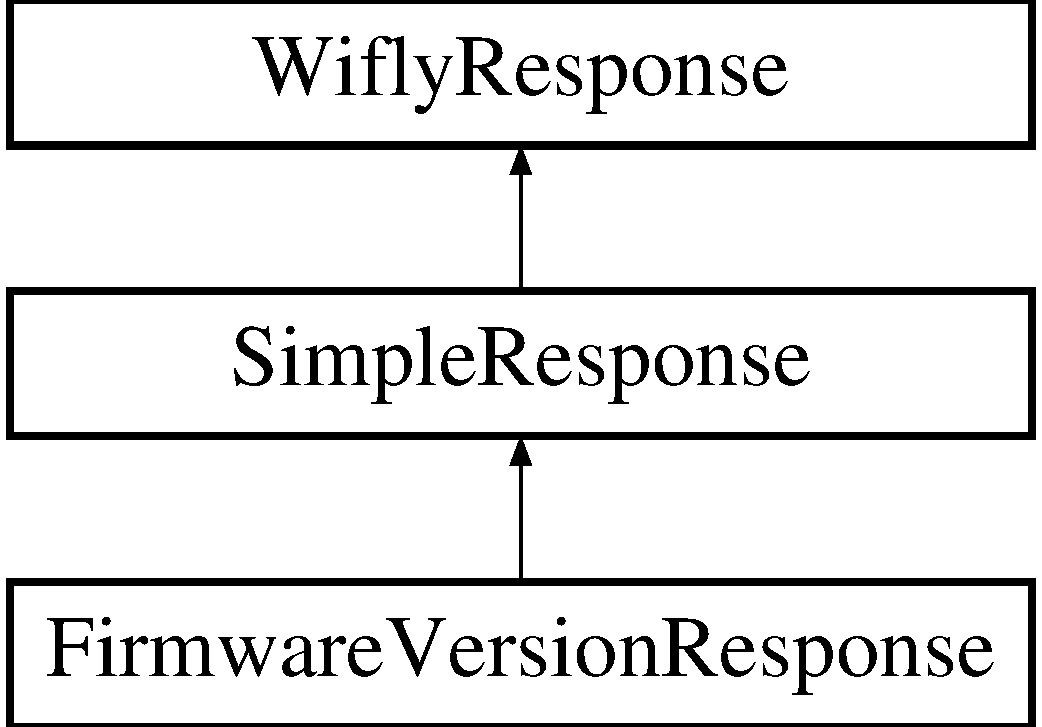
\includegraphics[height=3.000000cm]{class_firmware_version_response}
\end{center}
\end{figure}
\subsection*{Public Member Functions}
\begin{DoxyCompactItemize}
\item 
\hypertarget{class_firmware_version_response_a2abdf257bd1d7fb5c4cf9a005068173e}{void {\bfseries Init} (response\-\_\-frame $\ast$p\-Data, size\-\_\-t data\-Length)}\label{class_firmware_version_response_a2abdf257bd1d7fb5c4cf9a005068173e}

\end{DoxyCompactItemize}
\subsection*{Friends}
\begin{DoxyCompactItemize}
\item 
\hypertarget{class_firmware_version_response_a37b570544d9c72195251b87e598a0451}{std\-::ostream \& {\bfseries operator$<$$<$} (std\-::ostream \&out, const \hyperlink{class_firmware_version_response}{Firmware\-Version\-Response} \&ref)}\label{class_firmware_version_response_a37b570544d9c72195251b87e598a0451}

\end{DoxyCompactItemize}
\subsection*{Additional Inherited Members}


The documentation for this class was generated from the following file\-:\begin{DoxyCompactItemize}
\item 
library/Wifly\-Control\-Response.\-h\end{DoxyCompactItemize}

\hypertarget{class_fw_exception}{\section{Fw\-Exception Class Reference}
\label{class_fw_exception}\index{Fw\-Exception@{Fw\-Exception}}
}
Inheritance diagram for Fw\-Exception\-:\begin{figure}[H]
\begin{center}
\leavevmode
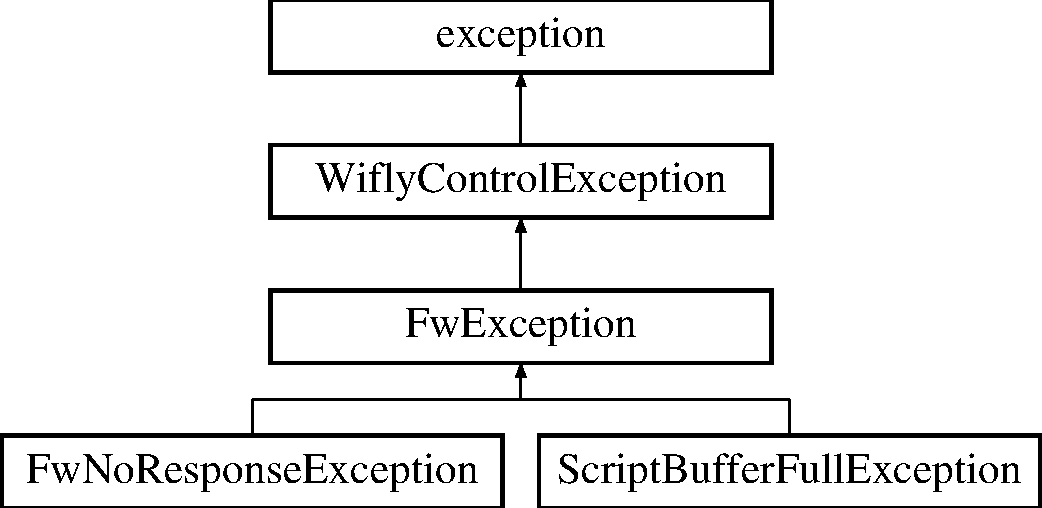
\includegraphics[height=4.000000cm]{class_fw_exception}
\end{center}
\end{figure}
\subsection*{Public Member Functions}
\begin{DoxyCompactItemize}
\item 
\hypertarget{class_fw_exception_a2ed0f0fded36da55c6ab89e84f690941}{{\bfseries Fw\-Exception} (const struct cmd\-\_\-frame $\ast$const failed\-Frame, const std\-::string error\-String)}\label{class_fw_exception_a2ed0f0fded36da55c6ab89e84f690941}

\item 
\hypertarget{class_fw_exception_af8b9d2e412bd11f40cc8b3964d6da13a}{struct cmd\-\_\-frame {\bfseries Get\-Failed\-Frame} (void) const }\label{class_fw_exception_af8b9d2e412bd11f40cc8b3964d6da13a}

\end{DoxyCompactItemize}


The documentation for this class was generated from the following file\-:\begin{DoxyCompactItemize}
\item 
library/Wifly\-Control\-Exception.\-h\end{DoxyCompactItemize}

\hypertarget{class_fw_no_response_exception}{\section{Fw\-No\-Response\-Exception Class Reference}
\label{class_fw_no_response_exception}\index{Fw\-No\-Response\-Exception@{Fw\-No\-Response\-Exception}}
}
Inheritance diagram for Fw\-No\-Response\-Exception\-:\begin{figure}[H]
\begin{center}
\leavevmode
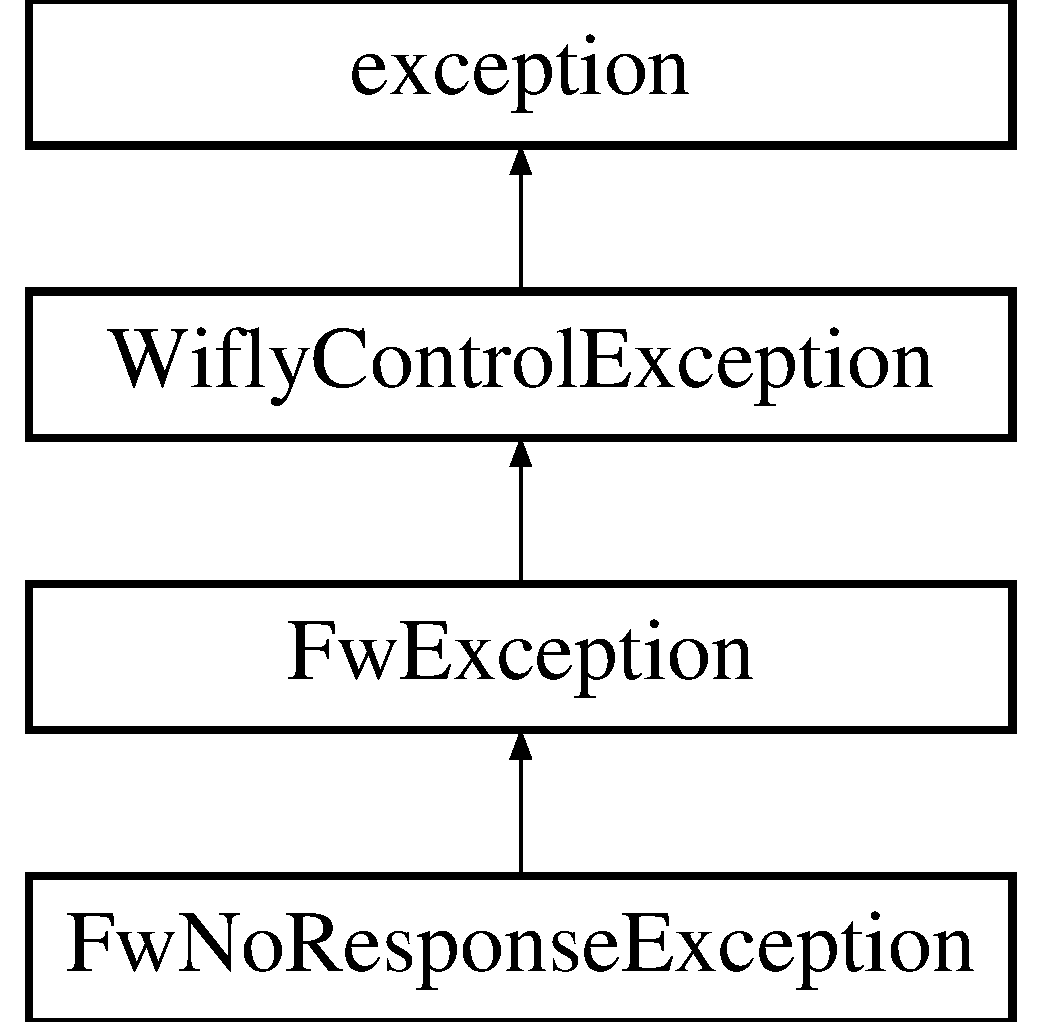
\includegraphics[height=4.000000cm]{class_fw_no_response_exception}
\end{center}
\end{figure}
\subsection*{Public Member Functions}
\begin{DoxyCompactItemize}
\item 
\hypertarget{class_fw_no_response_exception_ad34ddcad497c940499efcf7b138838c8}{{\bfseries Fw\-No\-Response\-Exception} (const struct cmd\-\_\-frame $\ast$const failed\-Command, const std\-::string error\-String=\char`\"{}Invalid response received or connection abort!\char`\"{})}\label{class_fw_no_response_exception_ad34ddcad497c940499efcf7b138838c8}

\end{DoxyCompactItemize}


The documentation for this class was generated from the following file\-:\begin{DoxyCompactItemize}
\item 
library/Wifly\-Control\-Exception.\-h\end{DoxyCompactItemize}

\hypertarget{classintelhex}{\section{intelhex Class Reference}
\label{classintelhex}\index{intelhex@{intelhex}}
}


Class to decode, encode and manipulate Intel H\-E\-X format files.  




{\ttfamily \#include $<$intelhexclass.\-h$>$}

\subsection*{Public Member Functions}
\begin{DoxyCompactItemize}
\item 
\hyperlink{classintelhex_ae1efd0ed1f56546f8f5f5af87c6cbdd5}{intelhex} ()
\begin{DoxyCompactList}\small\item\em intelhex Class Constructor. \end{DoxyCompactList}\item 
\hyperlink{classintelhex_a031ce4582899f5263fdcc2fa92cc3e45}{$\sim$intelhex} ()
\begin{DoxyCompactList}\small\item\em intelhex Class Deconstructor. \end{DoxyCompactList}\item 
\hyperlink{classintelhex_a41b4c3b7851461b9240fdef90bc62768}{intelhex} (const \hyperlink{classintelhex}{intelhex} \&ih\-Source)
\begin{DoxyCompactList}\small\item\em intelhex Class Copy Constructor. \end{DoxyCompactList}\item 
\hyperlink{classintelhex}{intelhex} \& \hyperlink{classintelhex_a6408cc3141862454e846378abfad8ecc}{operator=} (const \hyperlink{classintelhex}{intelhex} \&ih\-Source)
\begin{DoxyCompactList}\small\item\em intelhex Class Assignment Operator. \end{DoxyCompactList}\item 
\hyperlink{classintelhex}{intelhex} \& \hyperlink{classintelhex_a044d6ab5b10a38ffa40a0b1f55b7e808}{operator++} ()
\begin{DoxyCompactList}\small\item\em Overloaded prefix increment operator. \end{DoxyCompactList}\item 
const \hyperlink{classintelhex}{intelhex} \hyperlink{classintelhex_ab54337b9681fc0b50e3fdb18ed1714fa}{operator++} (int)
\begin{DoxyCompactList}\small\item\em Overloaded postfix increment operator. \end{DoxyCompactList}\item 
\hyperlink{classintelhex}{intelhex} \& \hyperlink{classintelhex_ab85cbeafe9cc6adcec79f1bc709addca}{operator-\/-\/} ()
\begin{DoxyCompactList}\small\item\em Overloaded prefix decrement operator. \end{DoxyCompactList}\item 
const \hyperlink{classintelhex}{intelhex} \hyperlink{classintelhex_a90562846d95b5573923f129b82aeceec}{operator-\/-\/} (int)
\begin{DoxyCompactList}\small\item\em Overloaded postfix decrement operator. \end{DoxyCompactList}\item 
void \hyperlink{classintelhex_ab2b1119e14a960ea2b356967244aafb3}{begin} ()
\begin{DoxyCompactList}\small\item\em Moves the address pointer to the first available address. \end{DoxyCompactList}\item 
void \hyperlink{classintelhex_a7759926596cfcffec94e391fff4298e9}{end} ()
\begin{DoxyCompactList}\small\item\em Moves the address pointer to the last available address. \end{DoxyCompactList}\item 
unsigned long \hyperlink{classintelhex_afa757932ec420f977d33bb9a2d5a0a69}{size} ()
\begin{DoxyCompactList}\small\item\em Checks if we have reached end of available data. \end{DoxyCompactList}\item 
bool \hyperlink{classintelhex_aff915b320f5a4c2d84340fa57c99499c}{end\-Of\-Data} ()
\begin{DoxyCompactList}\small\item\em Checks if we have reached end of available data. \end{DoxyCompactList}\item 
\hypertarget{classintelhex_a2bd5b567207303d4d9f4322e6262d6d6}{bool {\bfseries empty} ()}\label{classintelhex_a2bd5b567207303d4d9f4322e6262d6d6}

\item 
bool \hyperlink{classintelhex_a83b54457c121b0f35b21b78fa2ecd712}{jump\-To} (unsigned long address)
\begin{DoxyCompactList}\small\item\em Moves the address pointer to the desired address. \end{DoxyCompactList}\item 
bool \hyperlink{classintelhex_af9c6e296e5053fe8378e79445cf480cb}{increment\-Address} ()
\begin{DoxyCompactList}\small\item\em Increments to next piece of data. \end{DoxyCompactList}\item 
bool \hyperlink{classintelhex_a51f6d93f1ac2bdf5ddad8be4e1827ce9}{decrement\-Address} ()
\begin{DoxyCompactList}\small\item\em Decrements to next piece of data. \end{DoxyCompactList}\item 
unsigned long \hyperlink{classintelhex_a631d8930daeaf04bf0d9ad9c25679a0b}{current\-Address} ()
\begin{DoxyCompactList}\small\item\em Returns the current address being pointed to. \end{DoxyCompactList}\item 
bool \hyperlink{classintelhex_aa8833665b99f0b6ac64fcef7d2116c42}{start\-Address} (unsigned long $\ast$address)
\begin{DoxyCompactList}\small\item\em Returns the lowest address currently available. \end{DoxyCompactList}\item 
bool \hyperlink{classintelhex_a9b159bea81eb832e37f6cf88a57ca659}{end\-Address} (unsigned long $\ast$address)
\begin{DoxyCompactList}\small\item\em Returns the highest address currently available. \end{DoxyCompactList}\item 
bool \hyperlink{classintelhex_a01f7799f7a86e45c28b713e9472a8a5a}{get\-Data} (unsigned char $\ast$data)
\begin{DoxyCompactList}\small\item\em Returns the data to which the iterator is currently pointing. \end{DoxyCompactList}\item 
bool \hyperlink{classintelhex_a6596b518a9a832ed8e6ba21a0e07861c}{get\-Data} (unsigned char $\ast$data, unsigned long address)
\begin{DoxyCompactList}\small\item\em Returns the data for desired address. \end{DoxyCompactList}\item 
bool \hyperlink{classintelhex_a71096983db3c24a5ac9b95663937a4ce}{insert\-Data} (unsigned char data)
\begin{DoxyCompactList}\small\item\em Inserts desired byte at the current address pointer. \end{DoxyCompactList}\item 
\hypertarget{classintelhex_a00ff4c491fabc5ef207071358e1b9298}{bool {\bfseries insert\-Data} (unsigned char data, unsigned long address)}\label{classintelhex_a00ff4c491fabc5ef207071358e1b9298}

\item 
\hypertarget{classintelhex_ab4fc2715f4c63d3f31e8d2b0533583e5}{void {\bfseries overwrite\-Data} (unsigned char data)}\label{classintelhex_ab4fc2715f4c63d3f31e8d2b0533583e5}

\item 
\hypertarget{classintelhex_a83edcd2329cb52a4bab6bb46463184d7}{void {\bfseries overwrite\-Data} (unsigned char data, unsigned long address)}\label{classintelhex_a83edcd2329cb52a4bab6bb46463184d7}

\item 
\hypertarget{classintelhex_a5de5cf10103fc307127f9017f3e5cd76}{bool {\bfseries blank\-Fill} (unsigned char data)}\label{classintelhex_a5de5cf10103fc307127f9017f3e5cd76}

\item 
\hypertarget{classintelhex_a84bbd449bb55e218b62ea73e2b399196}{bool {\bfseries blank\-Fill} (unsigned char $\ast$const data, unsigned long size\-Of\-Data)}\label{classintelhex_a84bbd449bb55e218b62ea73e2b399196}

\item 
\hypertarget{classintelhex_aaf6f77af7a82623ef16471f105ac3fe7}{void {\bfseries blank\-Fill} (unsigned char $\ast$const data, unsigned long size\-Of\-Data, unsigned long \hyperlink{classintelhex_a9b159bea81eb832e37f6cf88a57ca659}{end\-Address})}\label{classintelhex_aaf6f77af7a82623ef16471f105ac3fe7}

\item 
\hypertarget{classintelhex_a9c26ba3dc9dd4f3021bb6c7f6983388f}{bool {\bfseries blank\-Fill\-Random} ()}\label{classintelhex_a9c26ba3dc9dd4f3021bb6c7f6983388f}

\item 
\hypertarget{classintelhex_aa1dbcbf3df1aaafd518882c882f43f76}{void {\bfseries blank\-Fill\-Random} (unsigned long \hyperlink{classintelhex_a9b159bea81eb832e37f6cf88a57ca659}{end\-Address})}\label{classintelhex_aa1dbcbf3df1aaafd518882c882f43f76}

\item 
\hypertarget{classintelhex_a2e5c67fccc34c78e6dbd28f4b795fb0f}{bool {\bfseries blank\-Fill\-Address\-Low\-Byte} ()}\label{classintelhex_a2e5c67fccc34c78e6dbd28f4b795fb0f}

\item 
\hypertarget{classintelhex_ab7b16f457563da93569b9812fafb9e7d}{void {\bfseries blank\-Fill\-Address\-Low\-Byte} (unsigned long \hyperlink{classintelhex_a9b159bea81eb832e37f6cf88a57ca659}{end\-Address})}\label{classintelhex_ab7b16f457563da93569b9812fafb9e7d}

\item 
unsigned long \hyperlink{classintelhex_a05a19e1e9f1eb493a8d0bc29db88683f}{get\-No\-Warnings} ()
\begin{DoxyCompactList}\small\item\em Returns number of unread warning messages. \end{DoxyCompactList}\item 
unsigned long \hyperlink{classintelhex_a77cddd46c3f97692b4d89f138bdabb72}{get\-No\-Errors} ()
\begin{DoxyCompactList}\small\item\em Returns number of unread error messages. \end{DoxyCompactList}\item 
bool \hyperlink{classintelhex_ab881b8cb0fe665395a29e4375db8f7c4}{pop\-Next\-Warning} (string \&warning)
\begin{DoxyCompactList}\small\item\em Pop next warning message from the list of warnings. \end{DoxyCompactList}\item 
bool \hyperlink{classintelhex_a6609fd1c57a650c45a1961f6318d643e}{pop\-Next\-Error} (string \&error)
\begin{DoxyCompactList}\small\item\em Pop next error message from the list of errors. \end{DoxyCompactList}\item 
bool \hyperlink{classintelhex_a94d6d17ba22263a4775d80b2a0e6e95f}{get\-Start\-Segment\-Address} (unsigned short $\ast$ip\-Register, unsigned short $\ast$cs\-Register)
\begin{DoxyCompactList}\small\item\em Returns segment start address for the I\-P and E\-S registers. \end{DoxyCompactList}\item 
bool \hyperlink{classintelhex_a7bc61f72756d37509e768906733ba10b}{get\-Start\-Linear\-Address} (unsigned long $\ast$eip\-Register)
\begin{DoxyCompactList}\small\item\em Returns segment linear address for the E\-I\-P register. \end{DoxyCompactList}\item 
void \hyperlink{classintelhex_a9688f0002be870b05d64b5f9fcdeb86b}{set\-Start\-Segment\-Address} (unsigned short ip\-Register, unsigned short cs\-Register)
\begin{DoxyCompactList}\small\item\em Sets the segment start address for the I\-P and C\-S registers. \end{DoxyCompactList}\item 
void \hyperlink{classintelhex_a7629ca097b2de02dea37fcaa2dc2709c}{set\-Start\-Linear\-Address} (unsigned long eip\-Register)
\begin{DoxyCompactList}\small\item\em Sets the segment start address for the E\-I\-P register. \end{DoxyCompactList}\item 
void \hyperlink{classintelhex_a489fc3b9c34542def2a5167192b291da}{segment\-Addressing\-On} ()
\begin{DoxyCompactList}\small\item\em Turns on segment addressing mode during encoding. \end{DoxyCompactList}\item 
void \hyperlink{classintelhex_a5055edd337d19037ab254a27016267f8}{linear\-Addressing\-On} ()
\begin{DoxyCompactList}\small\item\em Turns on linear addressing mode during encoding. \end{DoxyCompactList}\item 
void \hyperlink{classintelhex_ac6a0119a04a2090af3ffe8c33a37cbc9}{verbose\-On} ()
\begin{DoxyCompactList}\small\item\em Turns on textual output to cout during decoding. \end{DoxyCompactList}\item 
void \hyperlink{classintelhex_a3958f077a662291bbde3472ea2bcfb4d}{verbose\-Off} ()
\begin{DoxyCompactList}\small\item\em Turns off textual output to cout during decoding. \end{DoxyCompactList}\end{DoxyCompactItemize}
\subsection*{Friends}
\begin{DoxyCompactItemize}
\item 
ostream \& \hyperlink{classintelhex_a320e23dab311a6c652aa7ddb9e2f9cc2}{operator$<$$<$} (ostream \&data\-Out, \hyperlink{classintelhex}{intelhex} \&ih\-Local)
\begin{DoxyCompactList}\small\item\em Output stream overload operator. \end{DoxyCompactList}\item 
istream \& \hyperlink{classintelhex_a73fb9c5b9d6d069b5eb83340942fd54b}{operator$>$$>$} (istream \&data\-In, \hyperlink{classintelhex}{intelhex} \&ih\-Local)
\begin{DoxyCompactList}\small\item\em Input stream overload operator. \end{DoxyCompactList}\end{DoxyCompactItemize}


\subsection{Detailed Description}
Class to decode, encode and manipulate Intel H\-E\-X format files. 

The Intel H\-E\-X class allows the user to stream in the content of an Intel H\-E\-X file so that its content can by analysed more easily than trying to decode the Intel H\-E\-X file in a text editor. In conjunction with a suitable application it is possible to create content, analyse content and even compare the content of files with one another. 

\subsection{Constructor \& Destructor Documentation}
\hypertarget{classintelhex_ae1efd0ed1f56546f8f5f5af87c6cbdd5}{\index{intelhex@{intelhex}!intelhex@{intelhex}}
\index{intelhex@{intelhex}!intelhex@{intelhex}}
\subsubsection[{intelhex}]{\setlength{\rightskip}{0pt plus 5cm}intelhex\-::intelhex (
\begin{DoxyParamCaption}
{}
\end{DoxyParamCaption}
)\hspace{0.3cm}{\ttfamily [inline]}}}\label{classintelhex_ae1efd0ed1f56546f8f5f5af87c6cbdd5}


intelhex Class Constructor. 

Important initialisation steps performed here\-:
\begin{DoxyItemize}
\item clear segment base address to zero
\item clear all x86 start address registers to zero
\item note that there are, as yet, no errors or warnings
\item note that the E\-O\-F record has not yet been found
\item set verbode mode to 'false' (default)
\item initialise class ih\-Iterator 
\end{DoxyItemize}\hypertarget{classintelhex_a031ce4582899f5263fdcc2fa92cc3e45}{\index{intelhex@{intelhex}!$\sim$intelhex@{$\sim$intelhex}}
\index{$\sim$intelhex@{$\sim$intelhex}!intelhex@{intelhex}}
\subsubsection[{$\sim$intelhex}]{\setlength{\rightskip}{0pt plus 5cm}intelhex\-::$\sim$intelhex (
\begin{DoxyParamCaption}
{}
\end{DoxyParamCaption}
)\hspace{0.3cm}{\ttfamily [inline]}}}\label{classintelhex_a031ce4582899f5263fdcc2fa92cc3e45}


intelhex Class Deconstructor. 

Currently the deconstructor is intentially empty. \hypertarget{classintelhex_a41b4c3b7851461b9240fdef90bc62768}{\index{intelhex@{intelhex}!intelhex@{intelhex}}
\index{intelhex@{intelhex}!intelhex@{intelhex}}
\subsubsection[{intelhex}]{\setlength{\rightskip}{0pt plus 5cm}intelhex\-::intelhex (
\begin{DoxyParamCaption}
\item[{const {\bf intelhex} \&}]{ih\-Source}
\end{DoxyParamCaption}
)\hspace{0.3cm}{\ttfamily [inline]}}}\label{classintelhex_a41b4c3b7851461b9240fdef90bc62768}


intelhex Class Copy Constructor. 

Copy constructor copies all essential elements for the class. 

\subsection{Member Function Documentation}
\hypertarget{classintelhex_ab2b1119e14a960ea2b356967244aafb3}{\index{intelhex@{intelhex}!begin@{begin}}
\index{begin@{begin}!intelhex@{intelhex}}
\subsubsection[{begin}]{\setlength{\rightskip}{0pt plus 5cm}void intelhex\-::begin (
\begin{DoxyParamCaption}
{}
\end{DoxyParamCaption}
)\hspace{0.3cm}{\ttfamily [inline]}}}\label{classintelhex_ab2b1119e14a960ea2b356967244aafb3}


Moves the address pointer to the first available address. 

\begin{DoxyVerb}     The address pointer will be moved to the first available address in 
     memory of the decoded file or of the data the user has inserted into
     memory for the purpose of encoding into the Intel HEX format.
\end{DoxyVerb}


\begin{DoxySeeAlso}{See Also}
\hyperlink{classintelhex_a7759926596cfcffec94e391fff4298e9}{end()}
\end{DoxySeeAlso}
\begin{DoxyNote}{Note}
This function has no effect if no file has been as yet decoded and no data has been inserted into memory. 
\end{DoxyNote}
\hypertarget{classintelhex_a631d8930daeaf04bf0d9ad9c25679a0b}{\index{intelhex@{intelhex}!current\-Address@{current\-Address}}
\index{current\-Address@{current\-Address}!intelhex@{intelhex}}
\subsubsection[{current\-Address}]{\setlength{\rightskip}{0pt plus 5cm}unsigned long intelhex\-::current\-Address (
\begin{DoxyParamCaption}
{}
\end{DoxyParamCaption}
)\hspace{0.3cm}{\ttfamily [inline]}}}\label{classintelhex_a631d8930daeaf04bf0d9ad9c25679a0b}


Returns the current address being pointed to. 

\begin{DoxyVerb}     Current address will be returned.
\end{DoxyVerb}


\begin{DoxySeeAlso}{See Also}
\hyperlink{classintelhex_a83b54457c121b0f35b21b78fa2ecd712}{jump\-To()}
\end{DoxySeeAlso}

\begin{DoxyRetVals}{Return values}
{\em Current} & address being pointed to. \\
\hline
\end{DoxyRetVals}
\hypertarget{classintelhex_a51f6d93f1ac2bdf5ddad8be4e1827ce9}{\index{intelhex@{intelhex}!decrement\-Address@{decrement\-Address}}
\index{decrement\-Address@{decrement\-Address}!intelhex@{intelhex}}
\subsubsection[{decrement\-Address}]{\setlength{\rightskip}{0pt plus 5cm}bool intelhex\-::decrement\-Address (
\begin{DoxyParamCaption}
{}
\end{DoxyParamCaption}
)\hspace{0.3cm}{\ttfamily [inline]}}}\label{classintelhex_a51f6d93f1ac2bdf5ddad8be4e1827ce9}


Decrements to next piece of data. 

\begin{DoxyVerb}     Address pointer will take on the address of the previous location for 
     which there is data.
\end{DoxyVerb}


\begin{DoxySeeAlso}{See Also}
\hyperlink{classintelhex_af9c6e296e5053fe8378e79445cf480cb}{increment\-Address()}
\end{DoxySeeAlso}

\begin{DoxyRetVals}{Return values}
{\em true} & -\/ pointer was decremented; a new data value was found \\
\hline
{\em false} & -\/ start of available data reached; pointer is unchanged \\
\hline
\end{DoxyRetVals}
\hypertarget{classintelhex_a7759926596cfcffec94e391fff4298e9}{\index{intelhex@{intelhex}!end@{end}}
\index{end@{end}!intelhex@{intelhex}}
\subsubsection[{end}]{\setlength{\rightskip}{0pt plus 5cm}void intelhex\-::end (
\begin{DoxyParamCaption}
{}
\end{DoxyParamCaption}
)\hspace{0.3cm}{\ttfamily [inline]}}}\label{classintelhex_a7759926596cfcffec94e391fff4298e9}


Moves the address pointer to the last available address. 

\begin{DoxyVerb}     The address pointer will be moved to the last available address in 
     memory of the decoded file or of the data the user has inserted into
     memory for the purpose of encoding into the Intel HEX format.
\end{DoxyVerb}


\begin{DoxySeeAlso}{See Also}
\hyperlink{classintelhex_ab2b1119e14a960ea2b356967244aafb3}{begin()}
\end{DoxySeeAlso}
\begin{DoxyNote}{Note}
This function has no effect if no file has been as yet decoded and no data has been inserted into memory. 
\end{DoxyNote}
\hypertarget{classintelhex_a9b159bea81eb832e37f6cf88a57ca659}{\index{intelhex@{intelhex}!end\-Address@{end\-Address}}
\index{end\-Address@{end\-Address}!intelhex@{intelhex}}
\subsubsection[{end\-Address}]{\setlength{\rightskip}{0pt plus 5cm}bool intelhex\-::end\-Address (
\begin{DoxyParamCaption}
\item[{unsigned long $\ast$}]{address}
\end{DoxyParamCaption}
)\hspace{0.3cm}{\ttfamily [inline]}}}\label{classintelhex_a9b159bea81eb832e37f6cf88a57ca659}


Returns the highest address currently available. 

\begin{DoxyVerb}     Returns the last address that appears in the memory if there is data
     present. If not, no value will be returned.
\end{DoxyVerb}



\begin{DoxyParams}{Parameters}
{\em address} & -\/ variable to hold address requested\\
\hline
\end{DoxyParams}

\begin{DoxyRetVals}{Return values}
{\em true} & -\/ address existed and returned value is valid \\
\hline
{\em false} & -\/ address did not exist and returned valid is not valid\\
\hline
\end{DoxyRetVals}
\begin{DoxySeeAlso}{See Also}
\hyperlink{classintelhex_aa8833665b99f0b6ac64fcef7d2116c42}{start\-Address()} 
\end{DoxySeeAlso}
\hypertarget{classintelhex_aff915b320f5a4c2d84340fa57c99499c}{\index{intelhex@{intelhex}!end\-Of\-Data@{end\-Of\-Data}}
\index{end\-Of\-Data@{end\-Of\-Data}!intelhex@{intelhex}}
\subsubsection[{end\-Of\-Data}]{\setlength{\rightskip}{0pt plus 5cm}bool intelhex\-::end\-Of\-Data (
\begin{DoxyParamCaption}
{}
\end{DoxyParamCaption}
)\hspace{0.3cm}{\ttfamily [inline]}}}\label{classintelhex_aff915b320f5a4c2d84340fa57c99499c}


Checks if we have reached end of available data. 

\begin{DoxyVerb}     The internal pointer is checked to see if we have reached the end of 
     the data held in memory
\end{DoxyVerb}


\begin{DoxySeeAlso}{See Also}
\hyperlink{classintelhex_a044d6ab5b10a38ffa40a0b1f55b7e808}{operator++()}, \hyperlink{classintelhex_ab54337b9681fc0b50e3fdb18ed1714fa}{operator++(int)}, operator--(), operator--(int), empty()
\end{DoxySeeAlso}

\begin{DoxyRetVals}{Return values}
{\em true} & -\/ reached the end of the Intel H\-E\-X data in memory or no data in memory yet. \\
\hline
{\em false} & -\/ end of Intel H\-E\-X data in memory not yet reached.\\
\hline
\end{DoxyRetVals}
\begin{DoxyNote}{Note}
This function has no effect if no file has been as yet decoded and no data has been inserted into memory. 
\end{DoxyNote}
\hypertarget{classintelhex_a01f7799f7a86e45c28b713e9472a8a5a}{\index{intelhex@{intelhex}!get\-Data@{get\-Data}}
\index{get\-Data@{get\-Data}!intelhex@{intelhex}}
\subsubsection[{get\-Data}]{\setlength{\rightskip}{0pt plus 5cm}bool intelhex\-::get\-Data (
\begin{DoxyParamCaption}
\item[{unsigned char $\ast$}]{data}
\end{DoxyParamCaption}
)\hspace{0.3cm}{\ttfamily [inline]}}}\label{classintelhex_a01f7799f7a86e45c28b713e9472a8a5a}


Returns the data to which the iterator is currently pointing. 

\begin{DoxyVerb}     Returns the data to which the internal iterator (pointer) is currently
     pointing. If no data is in memory, this function returns false.
\end{DoxyVerb}



\begin{DoxyParams}{Parameters}
{\em data} & -\/ variable to hold data requested\\
\hline
\end{DoxyParams}

\begin{DoxyRetVals}{Return values}
{\em true} & -\/ data was available and returned value is valid \\
\hline
{\em false} & -\/ data was not available and returned valid is not valid\\
\hline
\end{DoxyRetVals}
\begin{DoxySeeAlso}{See Also}
put\-Data() 
\end{DoxySeeAlso}
\hypertarget{classintelhex_a6596b518a9a832ed8e6ba21a0e07861c}{\index{intelhex@{intelhex}!get\-Data@{get\-Data}}
\index{get\-Data@{get\-Data}!intelhex@{intelhex}}
\subsubsection[{get\-Data}]{\setlength{\rightskip}{0pt plus 5cm}bool intelhex\-::get\-Data (
\begin{DoxyParamCaption}
\item[{unsigned char $\ast$}]{data, }
\item[{unsigned long}]{address}
\end{DoxyParamCaption}
)\hspace{0.3cm}{\ttfamily [inline]}}}\label{classintelhex_a6596b518a9a832ed8e6ba21a0e07861c}


Returns the data for desired address. 

\begin{DoxyVerb}     Returns the data for the desired address. If the address has no data
     assigned to it, the function returns false, the pointer to data is not
     written and the class's address pointer remains unchanged. If the 
     address has data assigned to it, the pointer to data will be written 
     with the data found and the class's address pointer will be moved to 
     this new location.
\end{DoxyVerb}



\begin{DoxyParams}{Parameters}
{\em data} & -\/ variable to hold data requested \\
\hline
{\em address} & -\/ address to be queried for valid data\\
\hline
\end{DoxyParams}

\begin{DoxyRetVals}{Return values}
{\em true} & -\/ data was available and returned value is valid \\
\hline
{\em false} & -\/ data was not available and returned valid is not valid\\
\hline
\end{DoxyRetVals}
\begin{DoxySeeAlso}{See Also}
put\-Data() 
\end{DoxySeeAlso}
\hypertarget{classintelhex_a77cddd46c3f97692b4d89f138bdabb72}{\index{intelhex@{intelhex}!get\-No\-Errors@{get\-No\-Errors}}
\index{get\-No\-Errors@{get\-No\-Errors}!intelhex@{intelhex}}
\subsubsection[{get\-No\-Errors}]{\setlength{\rightskip}{0pt plus 5cm}unsigned long intelhex\-::get\-No\-Errors (
\begin{DoxyParamCaption}
{}
\end{DoxyParamCaption}
)\hspace{0.3cm}{\ttfamily [inline]}}}\label{classintelhex_a77cddd46c3f97692b4d89f138bdabb72}


Returns number of unread error messages. 

\begin{DoxyVerb}     Number of unread error messages will be returned.
\end{DoxyVerb}


\begin{DoxySeeAlso}{See Also}
\hyperlink{classintelhex_ab881b8cb0fe665395a29e4375db8f7c4}{pop\-Next\-Warning()}, \hyperlink{classintelhex_a05a19e1e9f1eb493a8d0bc29db88683f}{get\-No\-Warnings()}, \hyperlink{classintelhex_a6609fd1c57a650c45a1961f6318d643e}{pop\-Next\-Error()} 
\end{DoxySeeAlso}
\hypertarget{classintelhex_a05a19e1e9f1eb493a8d0bc29db88683f}{\index{intelhex@{intelhex}!get\-No\-Warnings@{get\-No\-Warnings}}
\index{get\-No\-Warnings@{get\-No\-Warnings}!intelhex@{intelhex}}
\subsubsection[{get\-No\-Warnings}]{\setlength{\rightskip}{0pt plus 5cm}unsigned long intelhex\-::get\-No\-Warnings (
\begin{DoxyParamCaption}
{}
\end{DoxyParamCaption}
)\hspace{0.3cm}{\ttfamily [inline]}}}\label{classintelhex_a05a19e1e9f1eb493a8d0bc29db88683f}


Returns number of unread warning messages. 

\begin{DoxyVerb}     Number of unread warning messages will be returned.
\end{DoxyVerb}


\begin{DoxySeeAlso}{See Also}
\hyperlink{classintelhex_ab881b8cb0fe665395a29e4375db8f7c4}{pop\-Next\-Warning()}, \hyperlink{classintelhex_a77cddd46c3f97692b4d89f138bdabb72}{get\-No\-Errors()}, \hyperlink{classintelhex_a6609fd1c57a650c45a1961f6318d643e}{pop\-Next\-Error()} 
\end{DoxySeeAlso}
\hypertarget{classintelhex_a7bc61f72756d37509e768906733ba10b}{\index{intelhex@{intelhex}!get\-Start\-Linear\-Address@{get\-Start\-Linear\-Address}}
\index{get\-Start\-Linear\-Address@{get\-Start\-Linear\-Address}!intelhex@{intelhex}}
\subsubsection[{get\-Start\-Linear\-Address}]{\setlength{\rightskip}{0pt plus 5cm}bool intelhex\-::get\-Start\-Linear\-Address (
\begin{DoxyParamCaption}
\item[{unsigned long $\ast$}]{eip\-Register}
\end{DoxyParamCaption}
)\hspace{0.3cm}{\ttfamily [inline]}}}\label{classintelhex_a7bc61f72756d37509e768906733ba10b}


Returns segment linear address for the E\-I\-P register. 

\begin{DoxyVerb}     If this value exists, they will be returned. If not, the function
     returns false.
\end{DoxyVerb}



\begin{DoxyParams}{Parameters}
{\em eip\-Register} & -\/ variable to store E\-I\-P register's value\\
\hline
\end{DoxyParams}

\begin{DoxyRetVals}{Return values}
{\em true} & -\/ E\-I\-P register has defined value \\
\hline
{\em false} & -\/ E\-I\-P register do not contain value\\
\hline
\end{DoxyRetVals}
\begin{DoxySeeAlso}{See Also}
\hyperlink{classintelhex_a94d6d17ba22263a4775d80b2a0e6e95f}{get\-Start\-Segment\-Address()}, \hyperlink{classintelhex_a9688f0002be870b05d64b5f9fcdeb86b}{set\-Start\-Segment\-Address()}, \hyperlink{classintelhex_a7629ca097b2de02dea37fcaa2dc2709c}{set\-Start\-Linear\-Address()} 
\end{DoxySeeAlso}
\hypertarget{classintelhex_a94d6d17ba22263a4775d80b2a0e6e95f}{\index{intelhex@{intelhex}!get\-Start\-Segment\-Address@{get\-Start\-Segment\-Address}}
\index{get\-Start\-Segment\-Address@{get\-Start\-Segment\-Address}!intelhex@{intelhex}}
\subsubsection[{get\-Start\-Segment\-Address}]{\setlength{\rightskip}{0pt plus 5cm}bool intelhex\-::get\-Start\-Segment\-Address (
\begin{DoxyParamCaption}
\item[{unsigned short $\ast$}]{ip\-Register, }
\item[{unsigned short $\ast$}]{cs\-Register}
\end{DoxyParamCaption}
)\hspace{0.3cm}{\ttfamily [inline]}}}\label{classintelhex_a94d6d17ba22263a4775d80b2a0e6e95f}


Returns segment start address for the I\-P and E\-S registers. 

\begin{DoxyVerb}     If these values exist, they will be returned. If not, the function
     returns false.
\end{DoxyVerb}



\begin{DoxyParams}{Parameters}
{\em ip\-Register} & -\/ variable to store I\-P register's value \\
\hline
{\em cs\-Register} & -\/ variable to store C\-S register's value\\
\hline
\end{DoxyParams}

\begin{DoxyRetVals}{Return values}
{\em true} & -\/ I\-P and C\-S registers have defined values \\
\hline
{\em false} & -\/ I\-P and C\-S registers do not contain values\\
\hline
\end{DoxyRetVals}
\begin{DoxySeeAlso}{See Also}
\hyperlink{classintelhex_a7bc61f72756d37509e768906733ba10b}{get\-Start\-Linear\-Address()}, \hyperlink{classintelhex_a9688f0002be870b05d64b5f9fcdeb86b}{set\-Start\-Segment\-Address()}, \hyperlink{classintelhex_a7629ca097b2de02dea37fcaa2dc2709c}{set\-Start\-Linear\-Address()} 
\end{DoxySeeAlso}
\hypertarget{classintelhex_af9c6e296e5053fe8378e79445cf480cb}{\index{intelhex@{intelhex}!increment\-Address@{increment\-Address}}
\index{increment\-Address@{increment\-Address}!intelhex@{intelhex}}
\subsubsection[{increment\-Address}]{\setlength{\rightskip}{0pt plus 5cm}bool intelhex\-::increment\-Address (
\begin{DoxyParamCaption}
{}
\end{DoxyParamCaption}
)\hspace{0.3cm}{\ttfamily [inline]}}}\label{classintelhex_af9c6e296e5053fe8378e79445cf480cb}


Increments to next piece of data. 

\begin{DoxyVerb}     Address pointer will take on the address of the next location for 
     which there is data.
\end{DoxyVerb}


\begin{DoxySeeAlso}{See Also}
\hyperlink{classintelhex_a51f6d93f1ac2bdf5ddad8be4e1827ce9}{decrement\-Address()}
\end{DoxySeeAlso}

\begin{DoxyRetVals}{Return values}
{\em true} & -\/ pointer was incremented; a new data value was found \\
\hline
{\em false} & -\/ end of available data reached; pointer is unchanged \\
\hline
\end{DoxyRetVals}
\hypertarget{classintelhex_a71096983db3c24a5ac9b95663937a4ce}{\index{intelhex@{intelhex}!insert\-Data@{insert\-Data}}
\index{insert\-Data@{insert\-Data}!intelhex@{intelhex}}
\subsubsection[{insert\-Data}]{\setlength{\rightskip}{0pt plus 5cm}bool intelhex\-::insert\-Data (
\begin{DoxyParamCaption}
\item[{unsigned char}]{data}
\end{DoxyParamCaption}
)}}\label{classintelhex_a71096983db3c24a5ac9b95663937a4ce}


Inserts desired byte at the current address pointer. 

\begin{DoxyVerb}     Inserts byte of data at the current address pointer
\end{DoxyVerb}



\begin{DoxyParams}{Parameters}
{\em data} & -\/ data byte to be inserted\\
\hline
\end{DoxyParams}
\begin{DoxySeeAlso}{See Also}
\hyperlink{classintelhex_aa8833665b99f0b6ac64fcef7d2116c42}{start\-Address()} 
\end{DoxySeeAlso}
\hypertarget{classintelhex_a83b54457c121b0f35b21b78fa2ecd712}{\index{intelhex@{intelhex}!jump\-To@{jump\-To}}
\index{jump\-To@{jump\-To}!intelhex@{intelhex}}
\subsubsection[{jump\-To}]{\setlength{\rightskip}{0pt plus 5cm}bool intelhex\-::jump\-To (
\begin{DoxyParamCaption}
\item[{unsigned long}]{address}
\end{DoxyParamCaption}
)\hspace{0.3cm}{\ttfamily [inline]}}}\label{classintelhex_a83b54457c121b0f35b21b78fa2ecd712}


Moves the address pointer to the desired address. 

\begin{DoxyVerb}     Address pointer will take on the requested address if the address
     exists in the data stored in memory. If not, the address pointer does
     not change.
\end{DoxyVerb}


\begin{DoxySeeAlso}{See Also}
\hyperlink{classintelhex_a631d8930daeaf04bf0d9ad9c25679a0b}{current\-Address()}
\end{DoxySeeAlso}

\begin{DoxyParams}{Parameters}
{\em address} & -\/ Desired new address for the address pointer\\
\hline
\end{DoxyParams}

\begin{DoxyRetVals}{Return values}
{\em true} & -\/ Address exists; pointer moved successfully \\
\hline
{\em false} & -\/ Address did not exist; pointer not moved \\
\hline
\end{DoxyRetVals}
\hypertarget{classintelhex_a5055edd337d19037ab254a27016267f8}{\index{intelhex@{intelhex}!linear\-Addressing\-On@{linear\-Addressing\-On}}
\index{linear\-Addressing\-On@{linear\-Addressing\-On}!intelhex@{intelhex}}
\subsubsection[{linear\-Addressing\-On}]{\setlength{\rightskip}{0pt plus 5cm}void intelhex\-::linear\-Addressing\-On (
\begin{DoxyParamCaption}
{}
\end{DoxyParamCaption}
)\hspace{0.3cm}{\ttfamily [inline]}}}\label{classintelhex_a5055edd337d19037ab254a27016267f8}


Turns on linear addressing mode during encoding. 

Uses the Linear Address Record during encoding. \hypertarget{classintelhex_a044d6ab5b10a38ffa40a0b1f55b7e808}{\index{intelhex@{intelhex}!operator++@{operator++}}
\index{operator++@{operator++}!intelhex@{intelhex}}
\subsubsection[{operator++}]{\setlength{\rightskip}{0pt plus 5cm}{\bf intelhex}\& intelhex\-::operator++ (
\begin{DoxyParamCaption}
{}
\end{DoxyParamCaption}
)\hspace{0.3cm}{\ttfamily [inline]}}}\label{classintelhex_a044d6ab5b10a38ffa40a0b1f55b7e808}


Overloaded prefix increment operator. 

Overloads the prefix increment operator to move interal iterator to next entry in the ih\-Content map \hypertarget{classintelhex_ab54337b9681fc0b50e3fdb18ed1714fa}{\index{intelhex@{intelhex}!operator++@{operator++}}
\index{operator++@{operator++}!intelhex@{intelhex}}
\subsubsection[{operator++}]{\setlength{\rightskip}{0pt plus 5cm}const {\bf intelhex} intelhex\-::operator++ (
\begin{DoxyParamCaption}
\item[{int}]{}
\end{DoxyParamCaption}
)\hspace{0.3cm}{\ttfamily [inline]}}}\label{classintelhex_ab54337b9681fc0b50e3fdb18ed1714fa}


Overloaded postfix increment operator. 

Overloads the postfix increment operator to move interal iterator to next entry in the ih\-Content map \hypertarget{classintelhex_ab85cbeafe9cc6adcec79f1bc709addca}{\index{intelhex@{intelhex}!operator-\/-\/@{operator-\/-\/}}
\index{operator-\/-\/@{operator-\/-\/}!intelhex@{intelhex}}
\subsubsection[{operator-\/-\/}]{\setlength{\rightskip}{0pt plus 5cm}{\bf intelhex}\& intelhex\-::operator-\/-\/ (
\begin{DoxyParamCaption}
{}
\end{DoxyParamCaption}
)\hspace{0.3cm}{\ttfamily [inline]}}}\label{classintelhex_ab85cbeafe9cc6adcec79f1bc709addca}


Overloaded prefix decrement operator. 

Overloads the prefix decrement operator to move interal iterator to previous entry in the ih\-Content map \hypertarget{classintelhex_a90562846d95b5573923f129b82aeceec}{\index{intelhex@{intelhex}!operator-\/-\/@{operator-\/-\/}}
\index{operator-\/-\/@{operator-\/-\/}!intelhex@{intelhex}}
\subsubsection[{operator-\/-\/}]{\setlength{\rightskip}{0pt plus 5cm}const {\bf intelhex} intelhex\-::operator-\/-\/ (
\begin{DoxyParamCaption}
\item[{int}]{}
\end{DoxyParamCaption}
)\hspace{0.3cm}{\ttfamily [inline]}}}\label{classintelhex_a90562846d95b5573923f129b82aeceec}


Overloaded postfix decrement operator. 

Overloads the postfix decrement operator to move interal iterator to previous entry in the ih\-Content map \hypertarget{classintelhex_a6408cc3141862454e846378abfad8ecc}{\index{intelhex@{intelhex}!operator=@{operator=}}
\index{operator=@{operator=}!intelhex@{intelhex}}
\subsubsection[{operator=}]{\setlength{\rightskip}{0pt plus 5cm}{\bf intelhex}\& intelhex\-::operator= (
\begin{DoxyParamCaption}
\item[{const {\bf intelhex} \&}]{ih\-Source}
\end{DoxyParamCaption}
)\hspace{0.3cm}{\ttfamily [inline]}}}\label{classintelhex_a6408cc3141862454e846378abfad8ecc}


intelhex Class Assignment Operator. 

\begin{DoxyVerb}     Implements the assignment operator so that the content of the Intel
     HEX file in memory can be copied to another 'intelhex' variable.
     You may want to keep a copy of the original data in memory and 
     only manipulate a copy.
\end{DoxyVerb}



\begin{DoxyParams}{Parameters}
{\em ih\-Source} & -\/ intelhex variable to be assigned to new variable\\
\hline
\end{DoxyParams}

\begin{DoxyRetVals}{Return values}
{\em pointer} & to variable to which value is to be assigned \\
\hline
\end{DoxyRetVals}
\hypertarget{classintelhex_a6609fd1c57a650c45a1961f6318d643e}{\index{intelhex@{intelhex}!pop\-Next\-Error@{pop\-Next\-Error}}
\index{pop\-Next\-Error@{pop\-Next\-Error}!intelhex@{intelhex}}
\subsubsection[{pop\-Next\-Error}]{\setlength{\rightskip}{0pt plus 5cm}bool intelhex\-::pop\-Next\-Error (
\begin{DoxyParamCaption}
\item[{string \&}]{error}
\end{DoxyParamCaption}
)\hspace{0.3cm}{\ttfamily [inline]}}}\label{classintelhex_a6609fd1c57a650c45a1961f6318d643e}


Pop next error message from the list of errors. 

\begin{DoxyVerb}     Next error message is returned from the list of errors. If there are
     no more errors in the list, no string will be returned unchanged.
\end{DoxyVerb}



\begin{DoxyParams}{Parameters}
{\em error} & -\/ variable to store error string to be returned\\
\hline
\end{DoxyParams}

\begin{DoxyRetVals}{Return values}
{\em true} & -\/ more error messages are available \\
\hline
{\em false} & -\/ no more error messages are available\\
\hline
\end{DoxyRetVals}
\begin{DoxySeeAlso}{See Also}
\hyperlink{classintelhex_a05a19e1e9f1eb493a8d0bc29db88683f}{get\-No\-Warnings()}, \hyperlink{classintelhex_a77cddd46c3f97692b4d89f138bdabb72}{get\-No\-Errors()}, \hyperlink{classintelhex_a6609fd1c57a650c45a1961f6318d643e}{pop\-Next\-Error()} 
\end{DoxySeeAlso}
\hypertarget{classintelhex_ab881b8cb0fe665395a29e4375db8f7c4}{\index{intelhex@{intelhex}!pop\-Next\-Warning@{pop\-Next\-Warning}}
\index{pop\-Next\-Warning@{pop\-Next\-Warning}!intelhex@{intelhex}}
\subsubsection[{pop\-Next\-Warning}]{\setlength{\rightskip}{0pt plus 5cm}bool intelhex\-::pop\-Next\-Warning (
\begin{DoxyParamCaption}
\item[{string \&}]{warning}
\end{DoxyParamCaption}
)\hspace{0.3cm}{\ttfamily [inline]}}}\label{classintelhex_ab881b8cb0fe665395a29e4375db8f7c4}


Pop next warning message from the list of warnings. 

\begin{DoxyVerb}     Next warning message is returned from the list of warnings. If there 
     are no more warning in the list, the string will be unchanged.
\end{DoxyVerb}



\begin{DoxyParams}{Parameters}
{\em warning} & -\/ variable to store warning string to be returned\\
\hline
\end{DoxyParams}

\begin{DoxyRetVals}{Return values}
{\em true} & -\/ more warning messages are available \\
\hline
{\em false} & -\/ no more warning messages are available\\
\hline
\end{DoxyRetVals}
\begin{DoxySeeAlso}{See Also}
\hyperlink{classintelhex_a05a19e1e9f1eb493a8d0bc29db88683f}{get\-No\-Warnings()}, \hyperlink{classintelhex_a77cddd46c3f97692b4d89f138bdabb72}{get\-No\-Errors()}, \hyperlink{classintelhex_a6609fd1c57a650c45a1961f6318d643e}{pop\-Next\-Error()} 
\end{DoxySeeAlso}
\hypertarget{classintelhex_a489fc3b9c34542def2a5167192b291da}{\index{intelhex@{intelhex}!segment\-Addressing\-On@{segment\-Addressing\-On}}
\index{segment\-Addressing\-On@{segment\-Addressing\-On}!intelhex@{intelhex}}
\subsubsection[{segment\-Addressing\-On}]{\setlength{\rightskip}{0pt plus 5cm}void intelhex\-::segment\-Addressing\-On (
\begin{DoxyParamCaption}
{}
\end{DoxyParamCaption}
)\hspace{0.3cm}{\ttfamily [inline]}}}\label{classintelhex_a489fc3b9c34542def2a5167192b291da}


Turns on segment addressing mode during encoding. 

Uses the Segment Address Record during encoding. \hypertarget{classintelhex_a7629ca097b2de02dea37fcaa2dc2709c}{\index{intelhex@{intelhex}!set\-Start\-Linear\-Address@{set\-Start\-Linear\-Address}}
\index{set\-Start\-Linear\-Address@{set\-Start\-Linear\-Address}!intelhex@{intelhex}}
\subsubsection[{set\-Start\-Linear\-Address}]{\setlength{\rightskip}{0pt plus 5cm}void intelhex\-::set\-Start\-Linear\-Address (
\begin{DoxyParamCaption}
\item[{unsigned long}]{eip\-Register}
\end{DoxyParamCaption}
)\hspace{0.3cm}{\ttfamily [inline]}}}\label{classintelhex_a7629ca097b2de02dea37fcaa2dc2709c}


Sets the segment start address for the E\-I\-P register. 

\begin{DoxyVerb}     Allows user to define or redefine the contents of the EIP register
\end{DoxyVerb}



\begin{DoxyParams}{Parameters}
{\em eip\-Register} & -\/ desired E\-I\-P register value\\
\hline
\end{DoxyParams}
\begin{DoxySeeAlso}{See Also}
\hyperlink{classintelhex_a94d6d17ba22263a4775d80b2a0e6e95f}{get\-Start\-Segment\-Address()}, \hyperlink{classintelhex_a9688f0002be870b05d64b5f9fcdeb86b}{set\-Start\-Segment\-Address()}, \hyperlink{classintelhex_a7bc61f72756d37509e768906733ba10b}{get\-Start\-Linear\-Address()} 
\end{DoxySeeAlso}
\hypertarget{classintelhex_a9688f0002be870b05d64b5f9fcdeb86b}{\index{intelhex@{intelhex}!set\-Start\-Segment\-Address@{set\-Start\-Segment\-Address}}
\index{set\-Start\-Segment\-Address@{set\-Start\-Segment\-Address}!intelhex@{intelhex}}
\subsubsection[{set\-Start\-Segment\-Address}]{\setlength{\rightskip}{0pt plus 5cm}void intelhex\-::set\-Start\-Segment\-Address (
\begin{DoxyParamCaption}
\item[{unsigned short}]{ip\-Register, }
\item[{unsigned short}]{cs\-Register}
\end{DoxyParamCaption}
)\hspace{0.3cm}{\ttfamily [inline]}}}\label{classintelhex_a9688f0002be870b05d64b5f9fcdeb86b}


Sets the segment start address for the I\-P and C\-S registers. 

\begin{DoxyVerb}     Allows user to define or redefine the contents of the IP and CS 
     registers
\end{DoxyVerb}



\begin{DoxyParams}{Parameters}
{\em ip\-Register} & -\/ desired I\-P register value \\
\hline
{\em cs\-Register} & -\/ desired C\-S register value\\
\hline
\end{DoxyParams}
\begin{DoxySeeAlso}{See Also}
\hyperlink{classintelhex_a7bc61f72756d37509e768906733ba10b}{get\-Start\-Linear\-Address()}, \hyperlink{classintelhex_a94d6d17ba22263a4775d80b2a0e6e95f}{get\-Start\-Segment\-Address()}, \hyperlink{classintelhex_a7629ca097b2de02dea37fcaa2dc2709c}{set\-Start\-Linear\-Address()} 
\end{DoxySeeAlso}
\hypertarget{classintelhex_afa757932ec420f977d33bb9a2d5a0a69}{\index{intelhex@{intelhex}!size@{size}}
\index{size@{size}!intelhex@{intelhex}}
\subsubsection[{size}]{\setlength{\rightskip}{0pt plus 5cm}unsigned long intelhex\-::size (
\begin{DoxyParamCaption}
{}
\end{DoxyParamCaption}
)\hspace{0.3cm}{\ttfamily [inline]}}}\label{classintelhex_afa757932ec420f977d33bb9a2d5a0a69}


Checks if we have reached end of available data. 

\begin{DoxyVerb}     The internal pointer is checked to see if we have reached the end of 
     the data held in memory
\end{DoxyVerb}


\begin{DoxySeeAlso}{See Also}
\hyperlink{classintelhex_a044d6ab5b10a38ffa40a0b1f55b7e808}{operator++()}, \hyperlink{classintelhex_ab54337b9681fc0b50e3fdb18ed1714fa}{operator++(int)}, operator--(), operator--(int), empty()
\end{DoxySeeAlso}

\begin{DoxyRetVals}{Return values}
{\em true} & -\/ reached the end of the Intel H\-E\-X data in memory or no data in memory yet. \\
\hline
{\em false} & -\/ end of Intel H\-E\-X data in memory not yet reached.\\
\hline
\end{DoxyRetVals}
\begin{DoxyNote}{Note}
This function has no effect if no file has been as yet decoded and no data has been inserted into memory. 
\end{DoxyNote}
\hypertarget{classintelhex_aa8833665b99f0b6ac64fcef7d2116c42}{\index{intelhex@{intelhex}!start\-Address@{start\-Address}}
\index{start\-Address@{start\-Address}!intelhex@{intelhex}}
\subsubsection[{start\-Address}]{\setlength{\rightskip}{0pt plus 5cm}bool intelhex\-::start\-Address (
\begin{DoxyParamCaption}
\item[{unsigned long $\ast$}]{address}
\end{DoxyParamCaption}
)\hspace{0.3cm}{\ttfamily [inline]}}}\label{classintelhex_aa8833665b99f0b6ac64fcef7d2116c42}


Returns the lowest address currently available. 

\begin{DoxyVerb}     Returns the first address that appears in the memory if there is data
     present. If not, no value will be returned.
\end{DoxyVerb}


\begin{DoxySeeAlso}{See Also}
\hyperlink{classintelhex_a9b159bea81eb832e37f6cf88a57ca659}{end\-Address()}
\end{DoxySeeAlso}

\begin{DoxyParams}{Parameters}
{\em address} & -\/ variable to hold address requested\\
\hline
\end{DoxyParams}

\begin{DoxyRetVals}{Return values}
{\em true} & -\/ address existed and returned value is valid \\
\hline
{\em false} & -\/ address did not exist and returned valid is not valid \\
\hline
\end{DoxyRetVals}
\hypertarget{classintelhex_a3958f077a662291bbde3472ea2bcfb4d}{\index{intelhex@{intelhex}!verbose\-Off@{verbose\-Off}}
\index{verbose\-Off@{verbose\-Off}!intelhex@{intelhex}}
\subsubsection[{verbose\-Off}]{\setlength{\rightskip}{0pt plus 5cm}void intelhex\-::verbose\-Off (
\begin{DoxyParamCaption}
{}
\end{DoxyParamCaption}
)\hspace{0.3cm}{\ttfamily [inline]}}}\label{classintelhex_a3958f077a662291bbde3472ea2bcfb4d}


Turns off textual output to cout during decoding. 

No output to cout during decoding of Intel H\-E\-X files. \hypertarget{classintelhex_ac6a0119a04a2090af3ffe8c33a37cbc9}{\index{intelhex@{intelhex}!verbose\-On@{verbose\-On}}
\index{verbose\-On@{verbose\-On}!intelhex@{intelhex}}
\subsubsection[{verbose\-On}]{\setlength{\rightskip}{0pt plus 5cm}void intelhex\-::verbose\-On (
\begin{DoxyParamCaption}
{}
\end{DoxyParamCaption}
)\hspace{0.3cm}{\ttfamily [inline]}}}\label{classintelhex_ac6a0119a04a2090af3ffe8c33a37cbc9}


Turns on textual output to cout during decoding. 

Per record single line output to cout during decoding of Intel H\-E\-X files. 

\subsection{Friends And Related Function Documentation}
\hypertarget{classintelhex_a320e23dab311a6c652aa7ddb9e2f9cc2}{\index{intelhex@{intelhex}!operator$<$$<$@{operator$<$$<$}}
\index{operator$<$$<$@{operator$<$$<$}!intelhex@{intelhex}}
\subsubsection[{operator$<$$<$}]{\setlength{\rightskip}{0pt plus 5cm}ostream\& operator$<$$<$ (
\begin{DoxyParamCaption}
\item[{ostream \&}]{data\-Out, }
\item[{{\bf intelhex} \&}]{ih\-Local}
\end{DoxyParamCaption}
)\hspace{0.3cm}{\ttfamily [friend]}}}\label{classintelhex_a320e23dab311a6c652aa7ddb9e2f9cc2}


Output stream overload operator. 

\begin{DoxyVerb}     Operator overloaded to encode any data held in memory into the Intel
     HEX format for storage on disk                 
\end{DoxyVerb}


\begin{DoxySeeAlso}{See Also}
\hyperlink{classintelhex_a73fb9c5b9d6d069b5eb83340942fd54b}{operator$>$$>$()}
\end{DoxySeeAlso}

\begin{DoxyParams}{Parameters}
{\em data\-Out} & -\/ Output stream for to store the decoded file information \\
\hline
{\em ih\-Local} & -\/ Points to this class so that friend function has access to private class members\\
\hline
\end{DoxyParams}

\begin{DoxyRetVals}{Return values}
{\em -\/} & pointer to output stream \\
\hline
\end{DoxyRetVals}
\hypertarget{classintelhex_a73fb9c5b9d6d069b5eb83340942fd54b}{\index{intelhex@{intelhex}!operator$>$$>$@{operator$>$$>$}}
\index{operator$>$$>$@{operator$>$$>$}!intelhex@{intelhex}}
\subsubsection[{operator$>$$>$}]{\setlength{\rightskip}{0pt plus 5cm}istream\& operator$>$$>$ (
\begin{DoxyParamCaption}
\item[{istream \&}]{data\-In, }
\item[{{\bf intelhex} \&}]{ih\-Local}
\end{DoxyParamCaption}
)\hspace{0.3cm}{\ttfamily [friend]}}}\label{classintelhex_a73fb9c5b9d6d069b5eb83340942fd54b}


Input stream overload operator. 

\begin{DoxyVerb}     Operator overloaded to decode data streamed in from a file in the 
     Intel HEX format into memory                 
\end{DoxyVerb}


\begin{DoxySeeAlso}{See Also}
\hyperlink{classintelhex_a320e23dab311a6c652aa7ddb9e2f9cc2}{operator$<$$<$()}
\end{DoxySeeAlso}

\begin{DoxyParams}{Parameters}
{\em data\-In} & -\/ Input stream for the encoded file information \\
\hline
{\em ih\-Local} & -\/ Points to this class so that friend function has access to private class members\\
\hline
\end{DoxyParams}

\begin{DoxyRetVals}{Return values}
{\em -\/} & pointer to input stream \\
\hline
\end{DoxyRetVals}


The documentation for this class was generated from the following file\-:\begin{DoxyCompactItemize}
\item 
library/\hyperlink{intelhexclass_8h}{intelhexclass.\-h}\end{DoxyCompactItemize}

\hypertarget{class_rtc_response}{\section{Rtc\-Response Class Reference}
\label{class_rtc_response}\index{Rtc\-Response@{Rtc\-Response}}
}
Inheritance diagram for Rtc\-Response\-:\begin{figure}[H]
\begin{center}
\leavevmode
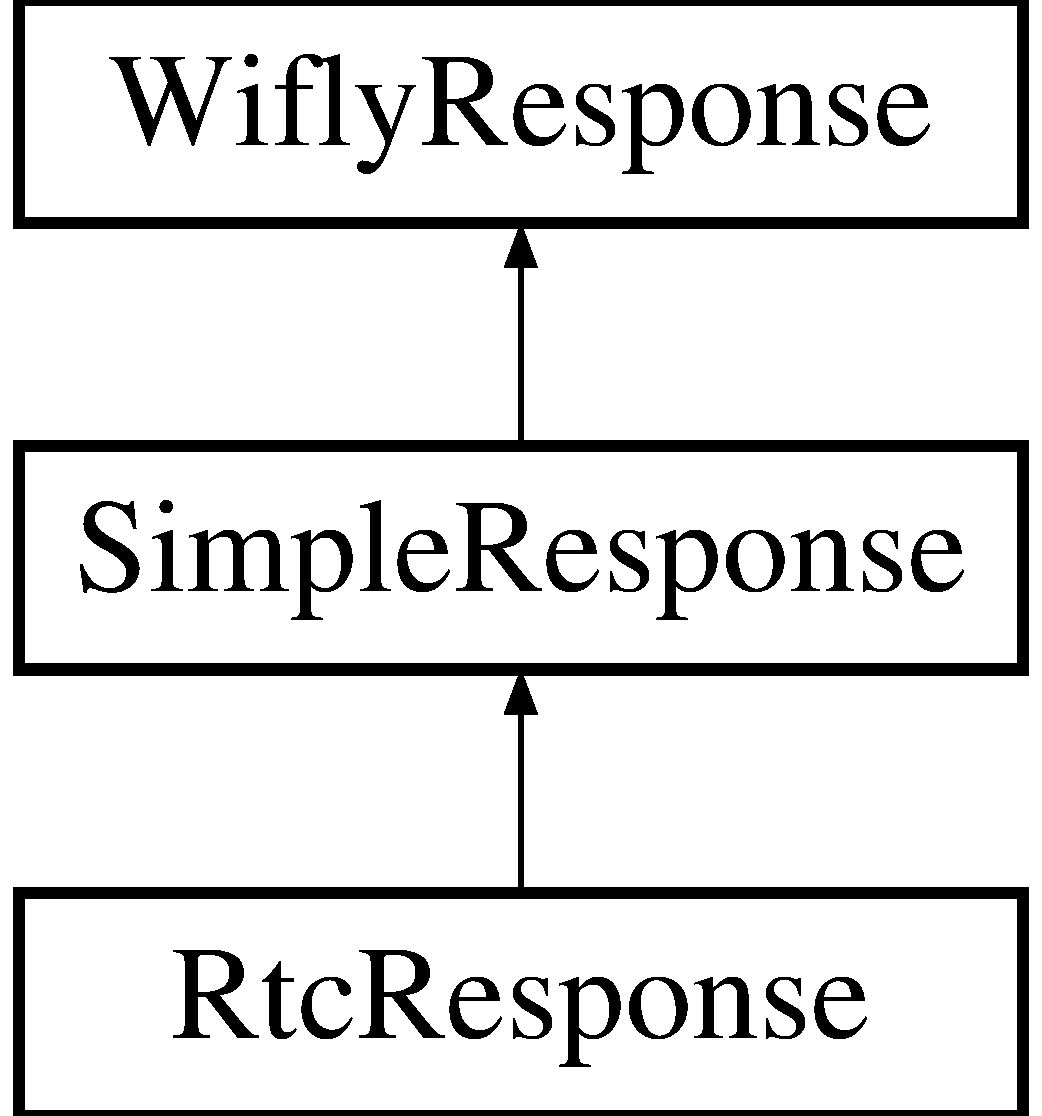
\includegraphics[height=3.000000cm]{class_rtc_response}
\end{center}
\end{figure}
\subsection*{Public Member Functions}
\begin{DoxyCompactItemize}
\item 
\hypertarget{class_rtc_response_ae5a5c5618830487cbc9d1197a47e3659}{void {\bfseries Init} (response\-\_\-frame $\ast$p\-Data, size\-\_\-t data\-Length)}\label{class_rtc_response_ae5a5c5618830487cbc9d1197a47e3659}

\item 
\hypertarget{class_rtc_response_abdf1aa92c47891e4ca9672a9244672a6}{struct tm {\bfseries Get\-Real\-Time} (void) const }\label{class_rtc_response_abdf1aa92c47891e4ca9672a9244672a6}

\end{DoxyCompactItemize}
\subsection*{Additional Inherited Members}


The documentation for this class was generated from the following file\-:\begin{DoxyCompactItemize}
\item 
library/Wifly\-Control\-Response.\-h\end{DoxyCompactItemize}

\hypertarget{class_script_buffer_full_exception}{\section{Script\-Buffer\-Full\-Exception Class Reference}
\label{class_script_buffer_full_exception}\index{Script\-Buffer\-Full\-Exception@{Script\-Buffer\-Full\-Exception}}
}
Inheritance diagram for Script\-Buffer\-Full\-Exception\-:\begin{figure}[H]
\begin{center}
\leavevmode
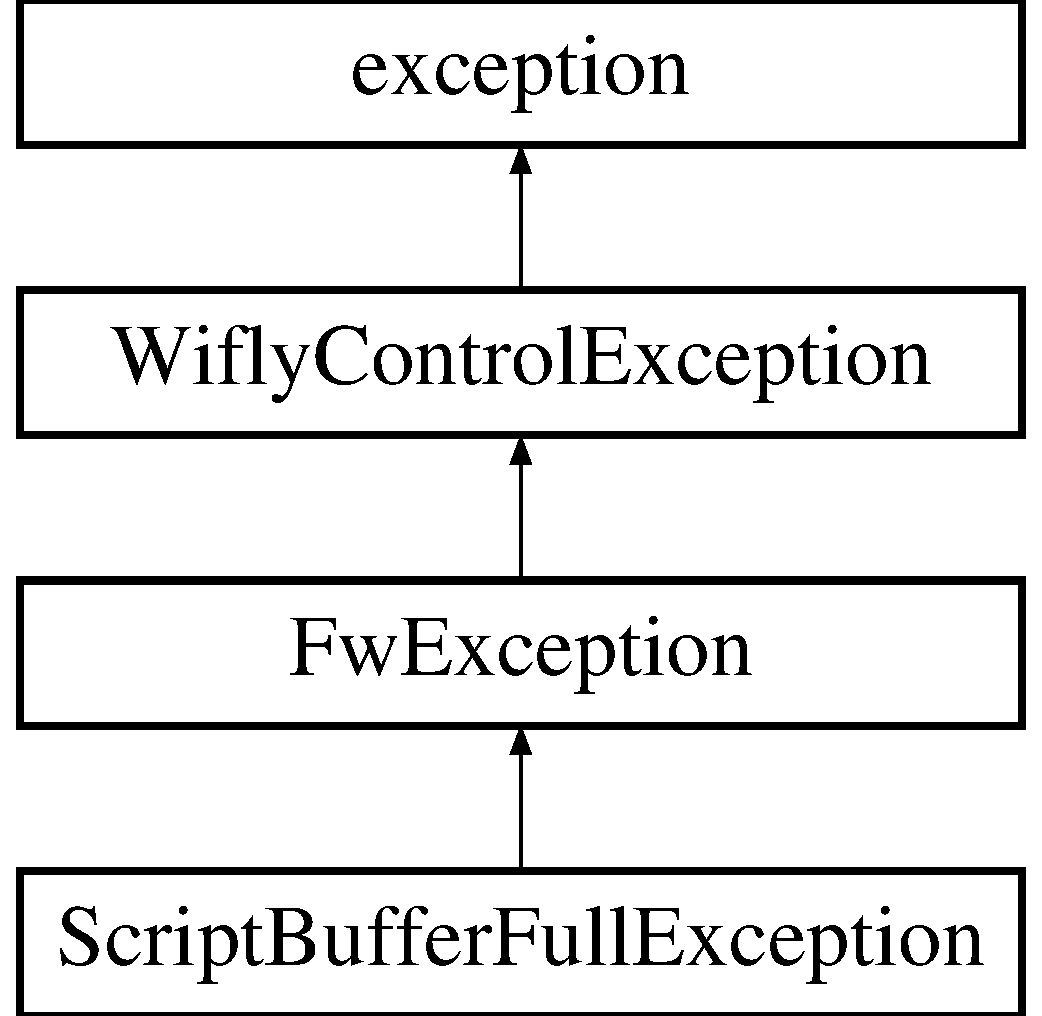
\includegraphics[height=4.000000cm]{class_script_buffer_full_exception}
\end{center}
\end{figure}
\subsection*{Public Member Functions}
\begin{DoxyCompactItemize}
\item 
\hypertarget{class_script_buffer_full_exception_ac7da5884fb0294041abf54a8b70283d2}{{\bfseries Script\-Buffer\-Full\-Exception} (const struct cmd\-\_\-frame $\ast$const failed\-Command, const std\-::string error\-String=\char`\"{}Buffer for commands in light is full!\char`\"{})}\label{class_script_buffer_full_exception_ac7da5884fb0294041abf54a8b70283d2}

\end{DoxyCompactItemize}


The documentation for this class was generated from the following file\-:\begin{DoxyCompactItemize}
\item 
library/Wifly\-Control\-Exception.\-h\end{DoxyCompactItemize}

\hypertarget{class_simple_response}{\section{Simple\-Response Class Reference}
\label{class_simple_response}\index{Simple\-Response@{Simple\-Response}}
}
Inheritance diagram for Simple\-Response\-:\begin{figure}[H]
\begin{center}
\leavevmode
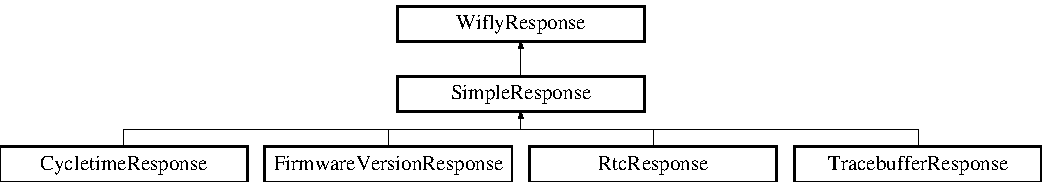
\includegraphics[height=2.441860cm]{class_simple_response}
\end{center}
\end{figure}
\subsection*{Public Member Functions}
\begin{DoxyCompactItemize}
\item 
\hypertarget{class_simple_response_aefac8d5010a3d168a206c78fbbd917ff}{{\bfseries Simple\-Response} (uint8\-\_\-t cmd)}\label{class_simple_response_aefac8d5010a3d168a206c78fbbd917ff}

\item 
\hypertarget{class_simple_response_a68f547257c77006d8dfc19192299b209}{void {\bfseries Init} (response\-\_\-frame $\ast$p\-Data, size\-\_\-t data\-Length)}\label{class_simple_response_a68f547257c77006d8dfc19192299b209}

\end{DoxyCompactItemize}
\subsection*{Additional Inherited Members}


The documentation for this class was generated from the following file\-:\begin{DoxyCompactItemize}
\item 
library/Wifly\-Control\-Response.\-h\end{DoxyCompactItemize}

\hypertarget{class_tcp_socket}{\section{Tcp\-Socket Class Reference}
\label{class_tcp_socket}\index{Tcp\-Socket@{Tcp\-Socket}}
}
Inheritance diagram for Tcp\-Socket\-:\begin{figure}[H]
\begin{center}
\leavevmode
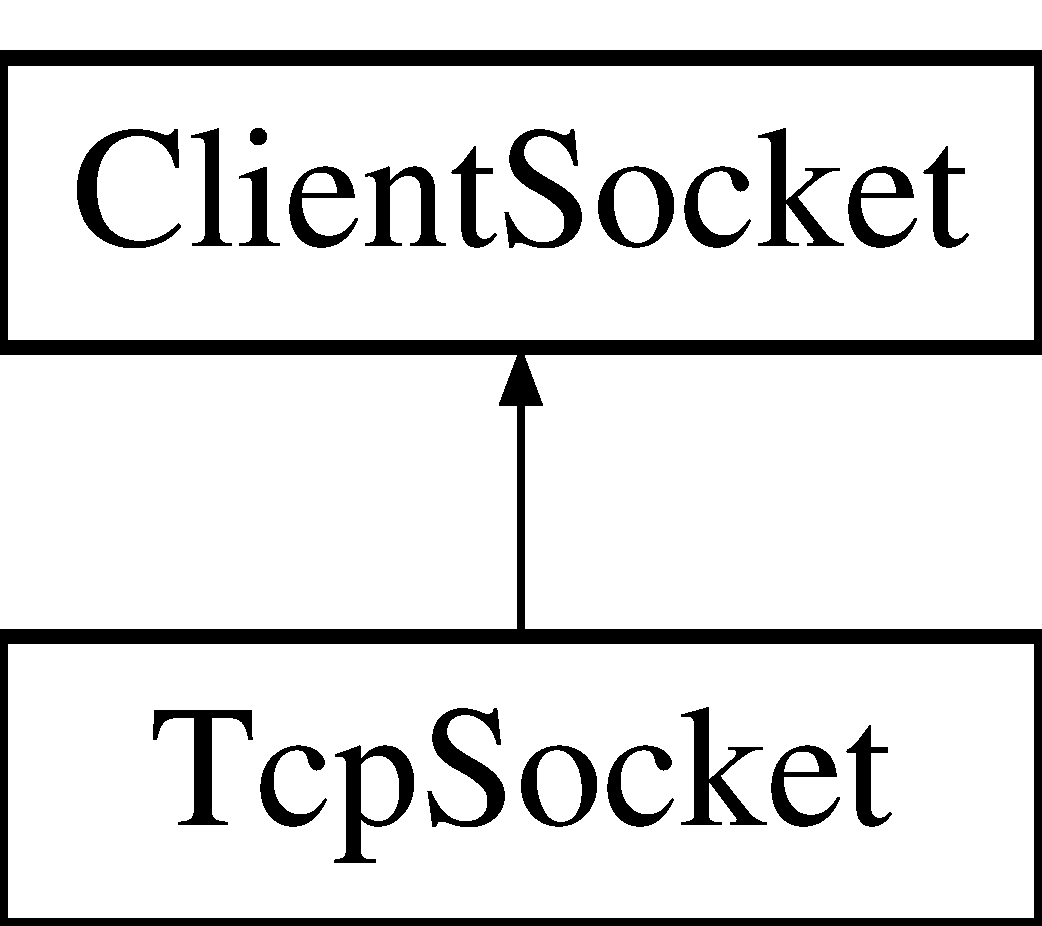
\includegraphics[height=2.000000cm]{class_tcp_socket}
\end{center}
\end{figure}
\subsection*{Public Member Functions}
\begin{DoxyCompactItemize}
\item 
\hypertarget{class_tcp_socket_ac7d0bc1afd5de6ed718785d35c656bb3}{{\bfseries Tcp\-Socket} (uint32\-\_\-t Addr, uint16\-\_\-t port)}\label{class_tcp_socket_ac7d0bc1afd5de6ed718785d35c656bb3}

\item 
size\-\_\-t \hyperlink{class_tcp_socket_ae11e390e4c9f9de484da2868a25d1623}{Recv} (uint8\-\_\-t $\ast$p\-Buffer, size\-\_\-t length, timeval $\ast$timeout=N\-U\-L\-L) const 
\item 
\hypertarget{class_tcp_socket_aadee07197b48fb7f50f7e9069fdb8d2d}{virtual size\-\_\-t {\bfseries Send} (const uint8\-\_\-t $\ast$frame, size\-\_\-t length) const }\label{class_tcp_socket_aadee07197b48fb7f50f7e9069fdb8d2d}

\end{DoxyCompactItemize}
\subsection*{Additional Inherited Members}


\subsection{Member Function Documentation}
\hypertarget{class_tcp_socket_ae11e390e4c9f9de484da2868a25d1623}{\index{Tcp\-Socket@{Tcp\-Socket}!Recv@{Recv}}
\index{Recv@{Recv}!TcpSocket@{Tcp\-Socket}}
\subsubsection[{Recv}]{\setlength{\rightskip}{0pt plus 5cm}size\-\_\-t Tcp\-Socket\-::\-Recv (
\begin{DoxyParamCaption}
\item[{uint8\-\_\-t $\ast$}]{p\-Buffer, }
\item[{size\-\_\-t}]{length, }
\item[{timeval $\ast$}]{timeout = {\ttfamily NULL}}
\end{DoxyParamCaption}
) const}}\label{class_tcp_socket_ae11e390e4c9f9de484da2868a25d1623}
For each call to \hyperlink{class_tcp_socket_ae11e390e4c9f9de484da2868a25d1623}{Recv()} we only return one byte of data to simulate a very fragmented response from pic. 

The documentation for this class was generated from the following files\-:\begin{DoxyCompactItemize}
\item 
library/Client\-Socket.\-h\item 
library/Client\-Socket.\-cpp\item 
library/Com\-Proxy\-\_\-ut.\-cpp\item 
library/Telnet\-Proxy\-\_\-ut.\-cpp\item 
library/Wifly\-Control\-\_\-ut.\-cpp\end{DoxyCompactItemize}

\hypertarget{class_telnet_proxy}{\section{Telnet\-Proxy Class Reference}
\label{class_telnet_proxy}\index{Telnet\-Proxy@{Telnet\-Proxy}}
}
\subsection*{Public Member Functions}
\begin{DoxyCompactItemize}
\item 
\hypertarget{class_telnet_proxy_aa7f9a2c3dffc0c3b7a2cb6f8e96a4645}{{\bfseries Telnet\-Proxy} (const \hyperlink{class_tcp_socket}{Tcp\-Socket} \&sock)}\label{class_telnet_proxy_aa7f9a2c3dffc0c3b7a2cb6f8e96a4645}

\item 
\hypertarget{class_telnet_proxy_a72cd6c477bcfc9a578ae3357f70ac1e5}{void {\bfseries Clear\-Response} (void) const }\label{class_telnet_proxy_a72cd6c477bcfc9a578ae3357f70ac1e5}

\item 
\hypertarget{class_telnet_proxy_ac06a0c97982e5c948f44eb1cabacf5c8}{bool {\bfseries Close} (bool do\-Save) const }\label{class_telnet_proxy_ac06a0c97982e5c948f44eb1cabacf5c8}

\item 
\hypertarget{class_telnet_proxy_a9f167bcd354e53ab8fb959472415762b}{void {\bfseries Recv\-String} (const std\-::string \&get\-Cmd, const std\-::string \&search\-Key, std\-::string \&result) const }\label{class_telnet_proxy_a9f167bcd354e53ab8fb959472415762b}

\item 
\hypertarget{class_telnet_proxy_a4b7729ca11f4ef533d3015b0a53974e6}{bool {\bfseries Open} (void) const }\label{class_telnet_proxy_a4b7729ca11f4ef533d3015b0a53974e6}

\item 
\hypertarget{class_telnet_proxy_a3a00f8fc67d35112929ca9e664c3197a}{bool {\bfseries Send} (const std\-::string \&telnet\-Message, const std\-::string \&expected\-Response=A\-O\-K) const }\label{class_telnet_proxy_a3a00f8fc67d35112929ca9e664c3197a}

\item 
\hypertarget{class_telnet_proxy_aa9ea9a5af4c1f58f2cc8c6edfa1501ae}{bool {\bfseries Send\-String} (const std\-::string \&command, std\-::string value) const }\label{class_telnet_proxy_aa9ea9a5af4c1f58f2cc8c6edfa1501ae}

\end{DoxyCompactItemize}
\subsection*{Friends}
\begin{DoxyCompactItemize}
\item 
\hypertarget{class_telnet_proxy_a436d76cf48d888700dddd5dc72c7bc56}{size\-\_\-t {\bfseries ut\-\_\-\-Telnet\-Proxy\-\_\-\-Recv} (void)}\label{class_telnet_proxy_a436d76cf48d888700dddd5dc72c7bc56}

\item 
\hypertarget{class_telnet_proxy_a899fd61cba9dec179f6a058b25c73cb7}{size\-\_\-t {\bfseries ut\-\_\-\-Telnet\-Proxy\-\_\-\-Recv\-String} (void)}\label{class_telnet_proxy_a899fd61cba9dec179f6a058b25c73cb7}

\end{DoxyCompactItemize}


The documentation for this class was generated from the following file\-:\begin{DoxyCompactItemize}
\item 
library/Telnet\-Proxy.\-h\end{DoxyCompactItemize}

\hypertarget{class_tracebuffer_response}{\section{Tracebuffer\-Response Class Reference}
\label{class_tracebuffer_response}\index{Tracebuffer\-Response@{Tracebuffer\-Response}}
}
Inheritance diagram for Tracebuffer\-Response\-:\begin{figure}[H]
\begin{center}
\leavevmode
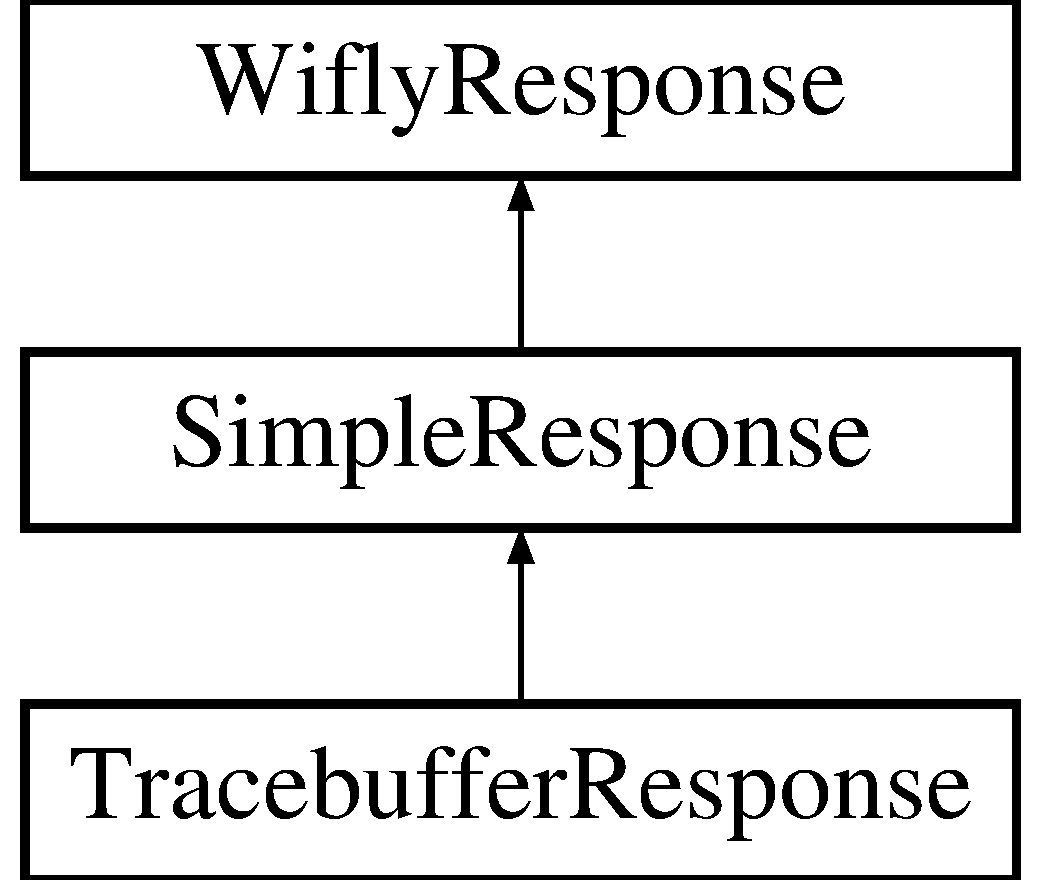
\includegraphics[height=3.000000cm]{class_tracebuffer_response}
\end{center}
\end{figure}
\subsection*{Public Member Functions}
\begin{DoxyCompactItemize}
\item 
\hypertarget{class_tracebuffer_response_aa091cf2da2f93d5be25386c91b827d72}{void {\bfseries Init} (response\-\_\-frame $\ast$p\-Data, size\-\_\-t data\-Length)}\label{class_tracebuffer_response_aa091cf2da2f93d5be25386c91b827d72}

\end{DoxyCompactItemize}
\subsection*{Friends}
\begin{DoxyCompactItemize}
\item 
\hypertarget{class_tracebuffer_response_a4ada06f1b6fe35635b6efdbbea164fd8}{std\-::ostream \& {\bfseries operator$<$$<$} (std\-::ostream \&out, const \hyperlink{class_tracebuffer_response}{Tracebuffer\-Response} \&ref)}\label{class_tracebuffer_response_a4ada06f1b6fe35635b6efdbbea164fd8}

\end{DoxyCompactItemize}
\subsection*{Additional Inherited Members}


The documentation for this class was generated from the following file\-:\begin{DoxyCompactItemize}
\item 
library/Wifly\-Control\-Response.\-h\end{DoxyCompactItemize}

\hypertarget{class_udp_socket}{\section{Udp\-Socket Class Reference}
\label{class_udp_socket}\index{Udp\-Socket@{Udp\-Socket}}
}
Inheritance diagram for Udp\-Socket\-:\begin{figure}[H]
\begin{center}
\leavevmode
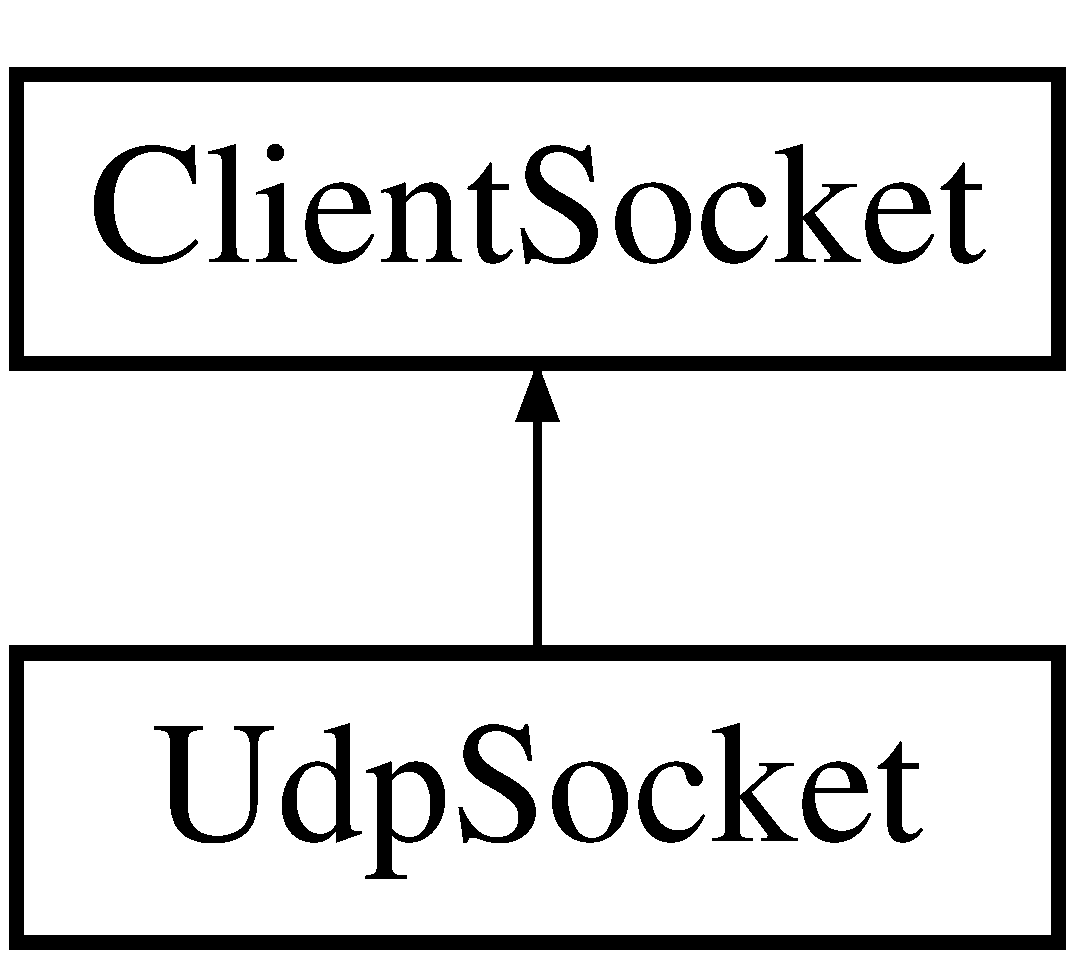
\includegraphics[height=2.000000cm]{class_udp_socket}
\end{center}
\end{figure}
\subsection*{Public Member Functions}
\begin{DoxyCompactItemize}
\item 
\hyperlink{class_udp_socket_a017a02140e8618ce88f8d8c5a3bf2ba3}{Udp\-Socket} (uint32\-\_\-t addr, uint16\-\_\-t port, bool do\-Bind=true, int enable\-Broadcast=0)
\item 
\hypertarget{class_udp_socket_a1391f69e42186e42966deb59c45f381f}{size\-\_\-t {\bfseries Recv\-From} (uint8\-\_\-t $\ast$p\-Buffer, size\-\_\-t length, timeval $\ast$timeout=N\-U\-L\-L, struct sockaddr $\ast$remote\-Addr=N\-U\-L\-L, socklen\-\_\-t $\ast$remote\-Addr\-Length=N\-U\-L\-L) const }\label{class_udp_socket_a1391f69e42186e42966deb59c45f381f}

\item 
\hypertarget{class_udp_socket_a8985c64bd6d8a3b10c51bb84df253c24}{virtual size\-\_\-t {\bfseries Send} (const uint8\-\_\-t $\ast$frame, size\-\_\-t length) const }\label{class_udp_socket_a8985c64bd6d8a3b10c51bb84df253c24}

\end{DoxyCompactItemize}
\subsection*{Additional Inherited Members}


\subsection{Constructor \& Destructor Documentation}
\hypertarget{class_udp_socket_a017a02140e8618ce88f8d8c5a3bf2ba3}{\index{Udp\-Socket@{Udp\-Socket}!Udp\-Socket@{Udp\-Socket}}
\index{Udp\-Socket@{Udp\-Socket}!UdpSocket@{Udp\-Socket}}
\subsubsection[{Udp\-Socket}]{\setlength{\rightskip}{0pt plus 5cm}Udp\-Socket\-::\-Udp\-Socket (
\begin{DoxyParamCaption}
\item[{uint32\-\_\-t}]{addr, }
\item[{uint16\-\_\-t}]{port, }
\item[{bool}]{do\-Bind = {\ttfamily true}, }
\item[{int}]{enable\-Broadcast = {\ttfamily 0}}
\end{DoxyParamCaption}
)}}\label{class_udp_socket_a017a02140e8618ce88f8d8c5a3bf2ba3}

\begin{DoxyParams}{Parameters}
{\em enable\-Broadcast} & use 1 to enable broadcast else set 0 \\
\hline
\end{DoxyParams}


The documentation for this class was generated from the following files\-:\begin{DoxyCompactItemize}
\item 
library/Client\-Socket.\-h\item 
library/Broadcast\-Receiver\-\_\-ut.\-cpp\item 
library/Client\-Socket.\-cpp\end{DoxyCompactItemize}

\hypertarget{class_wifly_color}{\section{Wifly\-Color Class Reference}
\label{class_wifly_color}\index{Wifly\-Color@{Wifly\-Color}}
}


{\ttfamily \#include $<$Wifly\-Color.\-h$>$}

\subsection*{Public Member Functions}
\begin{DoxyCompactItemize}
\item 
\hypertarget{class_wifly_color_a68d2fd89ce0c7d55514587c39f97e01c}{{\bfseries Wifly\-Color} (const uint32\-\_\-t argb\-Value=0)}\label{class_wifly_color_a68d2fd89ce0c7d55514587c39f97e01c}

\item 
\hypertarget{class_wifly_color_ad8523a03d716f35671c4e74f8940eb37}{uint8\-\_\-t {\bfseries red} () const }\label{class_wifly_color_ad8523a03d716f35671c4e74f8940eb37}

\item 
\hypertarget{class_wifly_color_a9397eca76be8f7abb88a84b719d99d6b}{void {\bfseries red} (uint8\-\_\-t value)}\label{class_wifly_color_a9397eca76be8f7abb88a84b719d99d6b}

\item 
\hypertarget{class_wifly_color_aeba066005ba425225621111ea6b9251f}{uint8\-\_\-t {\bfseries green} () const }\label{class_wifly_color_aeba066005ba425225621111ea6b9251f}

\item 
\hypertarget{class_wifly_color_abe50acffd7b1a172597ae8525149763a}{void {\bfseries green} (uint8\-\_\-t value)}\label{class_wifly_color_abe50acffd7b1a172597ae8525149763a}

\item 
\hypertarget{class_wifly_color_a9b2e0b29756d5915f4e96b85c1978fea}{uint8\-\_\-t {\bfseries blue} () const }\label{class_wifly_color_a9b2e0b29756d5915f4e96b85c1978fea}

\item 
\hypertarget{class_wifly_color_ad0c7f227f49eb00af032f4ae95e78f4a}{void {\bfseries blue} (uint8\-\_\-t value)}\label{class_wifly_color_ad0c7f227f49eb00af032f4ae95e78f4a}

\item 
\hypertarget{class_wifly_color_ac4034056a383f4e8c8beae0586459b8d}{uint32\-\_\-t {\bfseries argb} () const }\label{class_wifly_color_ac4034056a383f4e8c8beae0586459b8d}

\item 
\hypertarget{class_wifly_color_acfccad3c8a67c2e2f417beca040bc8df}{void {\bfseries argb} (uint32\-\_\-t argb\-Value)}\label{class_wifly_color_acfccad3c8a67c2e2f417beca040bc8df}

\end{DoxyCompactItemize}
\subsection*{Static Public Member Functions}
\begin{DoxyCompactItemize}
\item 
static uint32\-\_\-t \hyperlink{class_wifly_color_a0e552c6a422e953415700714ab9db184}{To\-A\-R\-G\-B} (const std\-::string \&s)
\end{DoxyCompactItemize}
\subsection*{Static Public Attributes}
\begin{DoxyCompactItemize}
\item 
\hypertarget{class_wifly_color_a9a00937bdf95435aa6e3e41ba5c6708b}{static const uint32\-\_\-t {\bfseries R\-E\-D} = 0xffff0000}\label{class_wifly_color_a9a00937bdf95435aa6e3e41ba5c6708b}

\item 
\hypertarget{class_wifly_color_adb9acf98ee5417f6293ae3fa9277237d}{static const uint32\-\_\-t {\bfseries G\-R\-E\-E\-N} = 0xff00ff00}\label{class_wifly_color_adb9acf98ee5417f6293ae3fa9277237d}

\item 
\hypertarget{class_wifly_color_ad63591638c12c2f9c5df743fceef6c43}{static const uint32\-\_\-t {\bfseries B\-L\-U\-E} = 0xff0000ff}\label{class_wifly_color_ad63591638c12c2f9c5df743fceef6c43}

\item 
\hypertarget{class_wifly_color_a746808c029beaa107b15296826f7e462}{static const uint32\-\_\-t {\bfseries W\-H\-I\-T\-E} = 0xffffffff}\label{class_wifly_color_a746808c029beaa107b15296826f7e462}

\item 
\hypertarget{class_wifly_color_afa045408a6b3f401e8b7d850f120a025}{static const uint32\-\_\-t {\bfseries B\-L\-A\-C\-K} = 0xff000000}\label{class_wifly_color_afa045408a6b3f401e8b7d850f120a025}

\end{DoxyCompactItemize}


\subsection{Detailed Description}
Copyright (C) 2012, 2013 Nils Weiss, Patrick Bruenn.

This file is part of Wifly\-\_\-\-Light.

Wifly\-\_\-\-Light is free software\-: you can redistribute it and/or modify it under the terms of the G\-N\-U General Public License as published by the Free Software Foundation, either version 3 of the License, or (at your option) any later version.

Wifly\-\_\-\-Light is distributed in the hope that it will be useful, but W\-I\-T\-H\-O\-U\-T A\-N\-Y W\-A\-R\-R\-A\-N\-T\-Y; without even the implied warranty of M\-E\-R\-C\-H\-A\-N\-T\-A\-B\-I\-L\-I\-T\-Y or F\-I\-T\-N\-E\-S\-S F\-O\-R A P\-A\-R\-T\-I\-C\-U\-L\-A\-R P\-U\-R\-P\-O\-S\-E. See the G\-N\-U General Public License for more details.

You should have received a copy of the G\-N\-U General Public License along with Wifly\-\_\-\-Light. If not, see \href{http://www.gnu.org/licenses/}{\tt http\-://www.\-gnu.\-org/licenses/}. 

\subsection{Member Function Documentation}
\hypertarget{class_wifly_color_a0e552c6a422e953415700714ab9db184}{\index{Wifly\-Color@{Wifly\-Color}!To\-A\-R\-G\-B@{To\-A\-R\-G\-B}}
\index{To\-A\-R\-G\-B@{To\-A\-R\-G\-B}!WiflyColor@{Wifly\-Color}}
\subsubsection[{To\-A\-R\-G\-B}]{\setlength{\rightskip}{0pt plus 5cm}static uint32\-\_\-t Wifly\-Color\-::\-To\-A\-R\-G\-B (
\begin{DoxyParamCaption}
\item[{const std\-::string \&}]{s}
\end{DoxyParamCaption}
)\hspace{0.3cm}{\ttfamily [inline]}, {\ttfamily [static]}}}\label{class_wifly_color_a0e552c6a422e953415700714ab9db184}
use a stringstream to convert hex ascii string into machine bits 

The documentation for this class was generated from the following file\-:\begin{DoxyCompactItemize}
\item 
library/Wifly\-Color.\-h\end{DoxyCompactItemize}

\hypertarget{class_wifly_control}{\section{Wifly\-Control Class Reference}
\label{class_wifly_control}\index{Wifly\-Control@{Wifly\-Control}}
}


{\ttfamily \#include $<$Wifly\-Control.\-h$>$}

\subsection*{Public Member Functions}
\begin{DoxyCompactItemize}
\item 
\hyperlink{class_wifly_control_a23f04e8c95cf5ebd5d576c0f6c5fecff}{Wifly\-Control} (uint32\-\_\-t addr, uint16\-\_\-t port)
\item 
void \hyperlink{class_wifly_control_a96bd445dcfcb45252530315b8919fd80}{Bl\-Eeprom\-Erase} (void) const 
\item 
void \hyperlink{class_wifly_control_acc372e780a40e0634d1ccf89aaba6b32}{Bl\-Enable\-Autostart} (void) const 
\item 
void \hyperlink{class_wifly_control_abe0bceb7ec0cfc88c2fccdae0d844d8a}{Bl\-Flash\-Erase} (void) const 
\item 
size\-\_\-t \hyperlink{class_wifly_control_a97f0c9d5e0ea08f2f60a720b0134fff1}{Bl\-Read\-Crc\-Flash} (uint8\-\_\-t $\ast$p\-Buffer, uint32\-\_\-t address, uint16\-\_\-t num\-Bytes) const 
\item 
size\-\_\-t \hyperlink{class_wifly_control_a13504dcf2d451545e8b5c3fa2f85b0e4}{Bl\-Read\-Eeprom} (uint8\-\_\-t $\ast$p\-Buffer, uint32\-\_\-t address, size\-\_\-t num\-Bytes) const 
\item 
size\-\_\-t \hyperlink{class_wifly_control_a5337818ba998047b8a8cdc738ddf3e43}{Bl\-Read\-Flash} (uint8\-\_\-t $\ast$p\-Buffer, uint32\-\_\-t address, size\-\_\-t num\-Bytes) const 
\item 
void \hyperlink{class_wifly_control_a26885cabebc9719b1da2d29131517efb}{Bl\-Read\-Info} (\hyperlink{struct_bl_info}{Bl\-Info} \&info) const 
\item 
void \hyperlink{class_wifly_control_a29e6124445a27e1fd26cfccce701cc09}{Bl\-Program\-Flash} (const std\-::string \&filename)
\item 
void \hyperlink{class_wifly_control_a776073bd4991e4331fb946e456d803df}{Bl\-Run\-App} (void) const 
\item 
std\-::string \hyperlink{class_wifly_control_aa46eb435216680bdb7e069571e7f7545}{Conf\-Get\-Ssid} (void) const 
\item 
bool \hyperlink{class_wifly_control_a932d65b7b9346a2bd9ced995fe2239ab}{Conf\-Set\-Defaults} (void) const 
\item 
bool \hyperlink{class_wifly_control_ad73ecaee1bf99c406c621fb602abf808}{Conf\-Set\-Wlan} (const std\-::string \&phrase, const std\-::string \&ssid) const 
\item 
void \hyperlink{class_wifly_control_a048e64bf80f176638032fec15f56c793}{Fw\-Clear\-Script} (\hyperlink{class_wifly_response}{Wifly\-Response} \&response)
\item 
\hyperlink{class_cycletime_response}{Cycletime\-Response} \& \hyperlink{class_wifly_control_aa909f4c3c1c02351197fa2bad8005a15}{Fw\-Get\-Cycletime} (\hyperlink{class_cycletime_response}{Cycletime\-Response} \&response)
\item 
void \hyperlink{class_wifly_control_a18b6f0a018f94aae19196fc0c2bc472c}{Fw\-Get\-Rtc} (\hyperlink{class_rtc_response}{Rtc\-Response} \&response)
\item 
\hyperlink{class_tracebuffer_response}{Tracebuffer\-Response} \& \hyperlink{class_wifly_control_ae5d32fb5569a4a4b8b9b5ea0df5ecc1d}{Fw\-Get\-Tracebuffer} (\hyperlink{class_tracebuffer_response}{Tracebuffer\-Response} \&response)
\item 
\hyperlink{class_firmware_version_response}{Firmware\-Version\-Response} \& \hyperlink{class_wifly_control_a8bfdeb73859dc3b95dd823e8b5c18514}{Fw\-Get\-Version} (\hyperlink{class_firmware_version_response}{Firmware\-Version\-Response} \&response)
\item 
void \hyperlink{class_wifly_control_ac0bcc3ca66256effb309545cf7341f9c}{Fw\-Loop\-On} (\hyperlink{class_wifly_response}{Wifly\-Response} \&response)
\item 
void \hyperlink{class_wifly_control_a8bcc4ce879e66a60f25c7790e07d3e61}{Fw\-Loop\-Off} (\hyperlink{class_wifly_response}{Wifly\-Response} \&response, uint8\-\_\-t num\-Loops)
\item 
void \hyperlink{class_wifly_control_a5a1bf514798ab57f893dbadfc525c531}{Fw\-Set\-Color\-Direct} (\hyperlink{class_wifly_response}{Wifly\-Response} \&response, uint8\-\_\-t $\ast$p\-Buffer, size\-\_\-t buffer\-Length)
\item 
void \hyperlink{class_wifly_control_a8f6ce3dc38f480fc68574f87983154ec}{Fw\-Set\-Fade} (\hyperlink{class_wifly_response}{Wifly\-Response} \&response, uint32\-\_\-t argb, uint16\-\_\-t fade\-Tmms=0, uint32\-\_\-t addr=0xffffffff, bool parallel\-Fade=false)
\item 
void \hyperlink{class_wifly_control_a9c09bac57cb017cb022b190616616975}{Fw\-Set\-Fade} (\hyperlink{class_wifly_response}{Wifly\-Response} \&response, const std\-::string \&rgb, uint16\-\_\-t fade\-Tmms=0, const std\-::string \&addr=\hyperlink{class_wifly_control_a1fb5f6703533d3ccf68f6e474f51dbce}{L\-E\-D\-S\-\_\-\-A\-L\-L}, bool parallel\-Fade=false)
\item 
void \hyperlink{class_wifly_control_a693a47088f11cba5659e3de44180f710}{Fw\-Set\-Rtc} (\hyperlink{class_simple_response}{Simple\-Response} \&response, struct tm $\ast$time\-Value)
\item 
void \hyperlink{class_wifly_control_a0caceaf85966349061bb6e435bfd557b}{Fw\-Set\-Wait} (\hyperlink{class_wifly_response}{Wifly\-Response} \&response, uint16\-\_\-t wait\-Tmms)
\item 
void \hyperlink{class_wifly_control_a155011ac62054bd61d9d29b6a6f5c2f3}{Fw\-Start\-Bl} (\hyperlink{class_simple_response}{Simple\-Response} \&response)
\item 
\hypertarget{class_wifly_control_ab7163d265422cb49fefc935da9e2857c}{void {\bfseries Fw\-Test} (void)}\label{class_wifly_control_ab7163d265422cb49fefc935da9e2857c}

\item 
\hypertarget{class_wifly_control_aa954fdf2ebcf00d628fc80231c2c4197}{void {\bfseries Fw\-Stress\-Test} (void)}\label{class_wifly_control_aa954fdf2ebcf00d628fc80231c2c4197}

\end{DoxyCompactItemize}
\subsection*{Static Public Attributes}
\begin{DoxyCompactItemize}
\item 
static const std\-::string \hyperlink{class_wifly_control_a1fb5f6703533d3ccf68f6e474f51dbce}{L\-E\-D\-S\-\_\-\-A\-L\-L} \{\char`\"{}ffffffff\char`\"{}\}
\end{DoxyCompactItemize}
\subsection*{Friends}
\begin{DoxyCompactItemize}
\item 
size\-\_\-t \hyperlink{class_wifly_control_a327c95f9335fa4b257b064ef2e917a80}{ut\-\_\-\-Wifly\-Control\-\_\-\-Bl\-Eeprom\-Write} (void)
\item 
\hypertarget{class_wifly_control_a661b9ec8a685bc800221f2fd5d031a20}{size\-\_\-t {\bfseries ut\-\_\-\-Wifly\-Control\-\_\-\-Bl\-Flash\-Write} (void)}\label{class_wifly_control_a661b9ec8a685bc800221f2fd5d031a20}

\end{DoxyCompactItemize}


\subsection{Detailed Description}
\begin{DoxyVerb}Copyright (C) 2012, 2013 Nils Weiss, Patrick Bruenn.
\end{DoxyVerb}


This file is part of Wifly\-\_\-\-Light.

Wifly\-\_\-\-Light is free software\-: you can redistribute it and/or modify it under the terms of the G\-N\-U General Public License as published by the Free Software Foundation, either version 3 of the License, or (at your option) any later version.

Wifly\-\_\-\-Light is distributed in the hope that it will be useful, but W\-I\-T\-H\-O\-U\-T A\-N\-Y W\-A\-R\-R\-A\-N\-T\-Y; without even the implied warranty of M\-E\-R\-C\-H\-A\-N\-T\-A\-B\-I\-L\-I\-T\-Y or F\-I\-T\-N\-E\-S\-S F\-O\-R A P\-A\-R\-T\-I\-C\-U\-L\-A\-R P\-U\-R\-P\-O\-S\-E. See the G\-N\-U General Public License for more details.

You should have received a copy of the G\-N\-U General Public License along with Wifly\-\_\-\-Light. If not, see \href{http://www.gnu.org/licenses/}{\tt http\-://www.\-gnu.\-org/licenses/}. 

\subsection{Constructor \& Destructor Documentation}
\hypertarget{class_wifly_control_a23f04e8c95cf5ebd5d576c0f6c5fecff}{\index{Wifly\-Control@{Wifly\-Control}!Wifly\-Control@{Wifly\-Control}}
\index{Wifly\-Control@{Wifly\-Control}!WiflyControl@{Wifly\-Control}}
\subsubsection[{Wifly\-Control}]{\setlength{\rightskip}{0pt plus 5cm}Wifly\-Control\-::\-Wifly\-Control (
\begin{DoxyParamCaption}
\item[{uint32\-\_\-t}]{addr, }
\item[{uint16\-\_\-t}]{port}
\end{DoxyParamCaption}
)}}\label{class_wifly_control_a23f04e8c95cf5ebd5d576c0f6c5fecff}
Connect to a wifly device 
\begin{DoxyParams}{Parameters}
{\em addr} & ipv4 address as 32 bit value in host byte order \\
\hline
{\em port} & number of the wifly device server in host byte order \\
\hline
\end{DoxyParams}


\subsection{Member Function Documentation}
\hypertarget{class_wifly_control_a96bd445dcfcb45252530315b8919fd80}{\index{Wifly\-Control@{Wifly\-Control}!Bl\-Eeprom\-Erase@{Bl\-Eeprom\-Erase}}
\index{Bl\-Eeprom\-Erase@{Bl\-Eeprom\-Erase}!WiflyControl@{Wifly\-Control}}
\subsubsection[{Bl\-Eeprom\-Erase}]{\setlength{\rightskip}{0pt plus 5cm}void Wifly\-Control\-::\-Bl\-Eeprom\-Erase (
\begin{DoxyParamCaption}
\item[{void}]{}
\end{DoxyParamCaption}
) const}}\label{class_wifly_control_a96bd445dcfcb45252530315b8919fd80}
-\/-\/-\/-\/-\/-\/-\/-\/-\/-\/-\/-\/-\/-\/-\/-\/-\/-\/-\/------ B\-O\-O\-T\-L\-O\-A\-D\-E\-R M\-E\-T\-H\-O\-D\-E\-S -\/-\/-\/-\/-\/-\/-\/-\/-\/-\/-\/-\/-\/-\/-\/-\/-\/-\/-\/------ Instructs the bootloader to erase the whole eeprom. The wifly device has to be in bootloader mode for this command.

-\/-\/-\/-\/-\/-\/-\/-\/-\/-\/-\/-\/-\/-\/-\/-\/-\/-\/-\/-\/-\/-\/--- B\-O\-O\-T\-L\-O\-A\-D\-E\-R M\-E\-T\-H\-O\-D\-E\-S -\/-\/-\/-\/-\/-\/-\/-\/-\/-\/-\/-\/-\/-\/-\/-\/-\/-\/-\/-\/-\/-\/--- \hypertarget{class_wifly_control_acc372e780a40e0634d1ccf89aaba6b32}{\index{Wifly\-Control@{Wifly\-Control}!Bl\-Enable\-Autostart@{Bl\-Enable\-Autostart}}
\index{Bl\-Enable\-Autostart@{Bl\-Enable\-Autostart}!WiflyControl@{Wifly\-Control}}
\subsubsection[{Bl\-Enable\-Autostart}]{\setlength{\rightskip}{0pt plus 5cm}void Wifly\-Control\-::\-Bl\-Enable\-Autostart (
\begin{DoxyParamCaption}
\item[{void}]{}
\end{DoxyParamCaption}
) const}}\label{class_wifly_control_acc372e780a40e0634d1ccf89aaba6b32}
Instructs the bootloader to set the autostart flag to true. This ensures the bootloader will be started on the next reboot automatically. \hypertarget{class_wifly_control_abe0bceb7ec0cfc88c2fccdae0d844d8a}{\index{Wifly\-Control@{Wifly\-Control}!Bl\-Flash\-Erase@{Bl\-Flash\-Erase}}
\index{Bl\-Flash\-Erase@{Bl\-Flash\-Erase}!WiflyControl@{Wifly\-Control}}
\subsubsection[{Bl\-Flash\-Erase}]{\setlength{\rightskip}{0pt plus 5cm}void Wifly\-Control\-::\-Bl\-Flash\-Erase (
\begin{DoxyParamCaption}
\item[{void}]{}
\end{DoxyParamCaption}
) const}}\label{class_wifly_control_abe0bceb7ec0cfc88c2fccdae0d844d8a}
Instructs the bootloader to erase the whole flash which is not occupied by the bootloader itself. The wifly device has to be in bootloader mode for this command. \hypertarget{class_wifly_control_a29e6124445a27e1fd26cfccce701cc09}{\index{Wifly\-Control@{Wifly\-Control}!Bl\-Program\-Flash@{Bl\-Program\-Flash}}
\index{Bl\-Program\-Flash@{Bl\-Program\-Flash}!WiflyControl@{Wifly\-Control}}
\subsubsection[{Bl\-Program\-Flash}]{\setlength{\rightskip}{0pt plus 5cm}void Wifly\-Control\-::\-Bl\-Program\-Flash (
\begin{DoxyParamCaption}
\item[{const std\-::string \&}]{filename}
\end{DoxyParamCaption}
)}}\label{class_wifly_control_a29e6124445a27e1fd26cfccce701cc09}
Instructs the bootloader to update the wifly device with new firmware. The wifly device has to be in bootloader mode for this command. 
\begin{DoxyParams}{Parameters}
{\em filename} & path to the $\ast$.hex file containing the new firmware \\
\hline
\end{DoxyParams}
\hypertarget{class_wifly_control_a97f0c9d5e0ea08f2f60a720b0134fff1}{\index{Wifly\-Control@{Wifly\-Control}!Bl\-Read\-Crc\-Flash@{Bl\-Read\-Crc\-Flash}}
\index{Bl\-Read\-Crc\-Flash@{Bl\-Read\-Crc\-Flash}!WiflyControl@{Wifly\-Control}}
\subsubsection[{Bl\-Read\-Crc\-Flash}]{\setlength{\rightskip}{0pt plus 5cm}size\-\_\-t Wifly\-Control\-::\-Bl\-Read\-Crc\-Flash (
\begin{DoxyParamCaption}
\item[{uint8\-\_\-t $\ast$}]{p\-Buffer, }
\item[{uint32\-\_\-t}]{address, }
\item[{uint16\-\_\-t}]{num\-Bytes}
\end{DoxyParamCaption}
) const}}\label{class_wifly_control_a97f0c9d5e0ea08f2f60a720b0134fff1}
Instructs the bootloader to create crc-\/16 checksums for the content of the specified flash area. T\-O\-D\-O crc values are in little endian byte order The wifly device has to be in bootloader mode for this command. 
\begin{DoxyParams}{Parameters}
{\em p\-Buffer} & pointer to a buffer for the resulting 16bit crc values \\
\hline
{\em address} & crc generation starts from this flash address \\
\hline
{\em num\-Bytes} & size of the flash area for which the crc are calculated \\
\hline
\end{DoxyParams}
\begin{DoxyReturn}{Returns}
the number of bytes read (result / 2 = number of crc values) 
\end{DoxyReturn}
\hypertarget{class_wifly_control_a13504dcf2d451545e8b5c3fa2f85b0e4}{\index{Wifly\-Control@{Wifly\-Control}!Bl\-Read\-Eeprom@{Bl\-Read\-Eeprom}}
\index{Bl\-Read\-Eeprom@{Bl\-Read\-Eeprom}!WiflyControl@{Wifly\-Control}}
\subsubsection[{Bl\-Read\-Eeprom}]{\setlength{\rightskip}{0pt plus 5cm}size\-\_\-t Wifly\-Control\-::\-Bl\-Read\-Eeprom (
\begin{DoxyParamCaption}
\item[{uint8\-\_\-t $\ast$}]{p\-Buffer, }
\item[{uint32\-\_\-t}]{address, }
\item[{size\-\_\-t}]{num\-Bytes}
\end{DoxyParamCaption}
) const}}\label{class_wifly_control_a13504dcf2d451545e8b5c3fa2f85b0e4}
Instructs the bootloader to read the specified memory area of the eeprom. The wifly device has to be in bootloader mode for this command. 
\begin{DoxyParams}{Parameters}
{\em p\-Buffer} & destination for the copy of the eeprom content, should be at least $<$num\-Bytes$>$ wide \\
\hline
{\em address} & start of the eeprom region to read \\
\hline
{\em num\-Bytes} & size of the eeprom region to read \\
\hline
\end{DoxyParams}
\begin{DoxyReturn}{Returns}
the number of bytes read 
\end{DoxyReturn}
\hypertarget{class_wifly_control_a5337818ba998047b8a8cdc738ddf3e43}{\index{Wifly\-Control@{Wifly\-Control}!Bl\-Read\-Flash@{Bl\-Read\-Flash}}
\index{Bl\-Read\-Flash@{Bl\-Read\-Flash}!WiflyControl@{Wifly\-Control}}
\subsubsection[{Bl\-Read\-Flash}]{\setlength{\rightskip}{0pt plus 5cm}size\-\_\-t Wifly\-Control\-::\-Bl\-Read\-Flash (
\begin{DoxyParamCaption}
\item[{uint8\-\_\-t $\ast$}]{p\-Buffer, }
\item[{uint32\-\_\-t}]{address, }
\item[{size\-\_\-t}]{num\-Bytes}
\end{DoxyParamCaption}
) const}}\label{class_wifly_control_a5337818ba998047b8a8cdc738ddf3e43}
Instructs the bootloader to read the specified memory area of the flash. The wifly device has to be in bootloader mode for this command. 
\begin{DoxyParams}{Parameters}
{\em p\-Buffer} & destination for the copy of the flash content, should be at least $<$num\-Bytes$>$ wide \\
\hline
{\em address} & start of the flash region to read\-Request \\
\hline
{\em numbytes} & size of the flash region to read \\
\hline
\end{DoxyParams}
\begin{DoxyReturn}{Returns}
the number of bytes read 
\end{DoxyReturn}
\hypertarget{class_wifly_control_a26885cabebc9719b1da2d29131517efb}{\index{Wifly\-Control@{Wifly\-Control}!Bl\-Read\-Info@{Bl\-Read\-Info}}
\index{Bl\-Read\-Info@{Bl\-Read\-Info}!WiflyControl@{Wifly\-Control}}
\subsubsection[{Bl\-Read\-Info}]{\setlength{\rightskip}{0pt plus 5cm}void Wifly\-Control\-::\-Bl\-Read\-Info (
\begin{DoxyParamCaption}
\item[{{\bf Bl\-Info} \&}]{info}
\end{DoxyParamCaption}
) const}}\label{class_wifly_control_a26885cabebc9719b1da2d29131517efb}
Instructs the bootloader to return a struct of bootloader informations like bootloader version, flash and eeprom size. see $<$\-Bl\-Info$>$ for details. The wifly device has to be in bootloader mode for this command. \hypertarget{class_wifly_control_a776073bd4991e4331fb946e456d803df}{\index{Wifly\-Control@{Wifly\-Control}!Bl\-Run\-App@{Bl\-Run\-App}}
\index{Bl\-Run\-App@{Bl\-Run\-App}!WiflyControl@{Wifly\-Control}}
\subsubsection[{Bl\-Run\-App}]{\setlength{\rightskip}{0pt plus 5cm}void Wifly\-Control\-::\-Bl\-Run\-App (
\begin{DoxyParamCaption}
\item[{void}]{}
\end{DoxyParamCaption}
) const}}\label{class_wifly_control_a776073bd4991e4331fb946e456d803df}
Instructs the bootloader to start the wifly device firmware. The wifly device has to be in bootloader mode for this command. \hypertarget{class_wifly_control_aa46eb435216680bdb7e069571e7f7545}{\index{Wifly\-Control@{Wifly\-Control}!Conf\-Get\-Ssid@{Conf\-Get\-Ssid}}
\index{Conf\-Get\-Ssid@{Conf\-Get\-Ssid}!WiflyControl@{Wifly\-Control}}
\subsubsection[{Conf\-Get\-Ssid}]{\setlength{\rightskip}{0pt plus 5cm}std\-::string Wifly\-Control\-::\-Conf\-Get\-Ssid (
\begin{DoxyParamCaption}
\item[{void}]{}
\end{DoxyParamCaption}
) const}}\label{class_wifly_control_aa46eb435216680bdb7e069571e7f7545}
-\/-\/-\/-\/-\/-\/-\/-\/-\/-\/-\/-\/-\/-\/-\/------ W\-L\-A\-N C\-O\-N\-F\-I\-G\-U\-R\-A\-T\-I\-O\-N M\-E\-T\-H\-O\-D\-E\-S -\/-\/-\/-\/-\/-\/-\/-\/-\/-\/-\/-\/-\/-\/-\/------ Read the currently configured ssid from Wifly module \begin{DoxyReturn}{Returns}
an empty string or the ssid 
\end{DoxyReturn}
\hypertarget{class_wifly_control_a932d65b7b9346a2bd9ced995fe2239ab}{\index{Wifly\-Control@{Wifly\-Control}!Conf\-Set\-Defaults@{Conf\-Set\-Defaults}}
\index{Conf\-Set\-Defaults@{Conf\-Set\-Defaults}!WiflyControl@{Wifly\-Control}}
\subsubsection[{Conf\-Set\-Defaults}]{\setlength{\rightskip}{0pt plus 5cm}bool Wifly\-Control\-::\-Conf\-Set\-Defaults (
\begin{DoxyParamCaption}
\item[{void}]{}
\end{DoxyParamCaption}
) const}}\label{class_wifly_control_a932d65b7b9346a2bd9ced995fe2239ab}
Set the Wifly module communication parameters to defaults \begin{DoxyReturn}{Returns}
false, in case of an error 
\end{DoxyReturn}
\hypertarget{class_wifly_control_ad73ecaee1bf99c406c621fb602abf808}{\index{Wifly\-Control@{Wifly\-Control}!Conf\-Set\-Wlan@{Conf\-Set\-Wlan}}
\index{Conf\-Set\-Wlan@{Conf\-Set\-Wlan}!WiflyControl@{Wifly\-Control}}
\subsubsection[{Conf\-Set\-Wlan}]{\setlength{\rightskip}{0pt plus 5cm}bool Wifly\-Control\-::\-Conf\-Set\-Wlan (
\begin{DoxyParamCaption}
\item[{const std\-::string \&}]{phrase, }
\item[{const std\-::string \&}]{ssid}
\end{DoxyParamCaption}
) const}}\label{class_wifly_control_ad73ecaee1bf99c406c621fb602abf808}
Set the Wifly module wlan connection parameters 
\begin{DoxyParams}{Parameters}
{\em phrase} & W\-P\-A2 passphrase 1 -\/ 63 characters \\
\hline
{\em ssid} & 1 -\/ 32 characters \\
\hline
\end{DoxyParams}
\begin{DoxyReturn}{Returns}
false, in case of an error 
\end{DoxyReturn}
\hypertarget{class_wifly_control_a048e64bf80f176638032fec15f56c793}{\index{Wifly\-Control@{Wifly\-Control}!Fw\-Clear\-Script@{Fw\-Clear\-Script}}
\index{Fw\-Clear\-Script@{Fw\-Clear\-Script}!WiflyControl@{Wifly\-Control}}
\subsubsection[{Fw\-Clear\-Script}]{\setlength{\rightskip}{0pt plus 5cm}void Wifly\-Control\-::\-Fw\-Clear\-Script (
\begin{DoxyParamCaption}
\item[{{\bf Wifly\-Response} \&}]{response}
\end{DoxyParamCaption}
)}}\label{class_wifly_control_a048e64bf80f176638032fec15f56c793}
-\/-\/-\/-\/-\/-\/-\/-\/-\/-\/-\/-\/-\/-\/-\/-\/-\/-\/-\/-\/------ F\-I\-R\-M\-W\-A\-R\-E M\-E\-T\-H\-O\-D\-E\-S -\/-\/-\/-\/-\/-\/-\/-\/-\/-\/-\/-\/-\/-\/-\/-\/-\/-\/-\/-\/------ Wipe all commands from the Wifly script controller 
\begin{DoxyParams}{Parameters}
{\em response} & will be modified according to the success of this operation \\
\hline
\end{DoxyParams}
\hypertarget{class_wifly_control_aa909f4c3c1c02351197fa2bad8005a15}{\index{Wifly\-Control@{Wifly\-Control}!Fw\-Get\-Cycletime@{Fw\-Get\-Cycletime}}
\index{Fw\-Get\-Cycletime@{Fw\-Get\-Cycletime}!WiflyControl@{Wifly\-Control}}
\subsubsection[{Fw\-Get\-Cycletime}]{\setlength{\rightskip}{0pt plus 5cm}{\bf Cycletime\-Response} \& Wifly\-Control\-::\-Fw\-Get\-Cycletime (
\begin{DoxyParamCaption}
\item[{{\bf Cycletime\-Response} \&}]{response}
\end{DoxyParamCaption}
)}}\label{class_wifly_control_aa909f4c3c1c02351197fa2bad8005a15}
Reads the cycletimes from wifly device and stores them into the response object 
\begin{DoxyParams}{Parameters}
{\em response} & reference to an object to store the read cyletimes \\
\hline
\end{DoxyParams}
\begin{DoxyReturn}{Returns}
$<$response$>$ 
\end{DoxyReturn}
\hypertarget{class_wifly_control_a18b6f0a018f94aae19196fc0c2bc472c}{\index{Wifly\-Control@{Wifly\-Control}!Fw\-Get\-Rtc@{Fw\-Get\-Rtc}}
\index{Fw\-Get\-Rtc@{Fw\-Get\-Rtc}!WiflyControl@{Wifly\-Control}}
\subsubsection[{Fw\-Get\-Rtc}]{\setlength{\rightskip}{0pt plus 5cm}void Wifly\-Control\-::\-Fw\-Get\-Rtc (
\begin{DoxyParamCaption}
\item[{{\bf Rtc\-Response} \&}]{response}
\end{DoxyParamCaption}
)}}\label{class_wifly_control_a18b6f0a018f94aae19196fc0c2bc472c}
Reads the current rtc time from the wifly device \hypertarget{class_wifly_control_ae5d32fb5569a4a4b8b9b5ea0df5ecc1d}{\index{Wifly\-Control@{Wifly\-Control}!Fw\-Get\-Tracebuffer@{Fw\-Get\-Tracebuffer}}
\index{Fw\-Get\-Tracebuffer@{Fw\-Get\-Tracebuffer}!WiflyControl@{Wifly\-Control}}
\subsubsection[{Fw\-Get\-Tracebuffer}]{\setlength{\rightskip}{0pt plus 5cm}{\bf Tracebuffer\-Response} \& Wifly\-Control\-::\-Fw\-Get\-Tracebuffer (
\begin{DoxyParamCaption}
\item[{{\bf Tracebuffer\-Response} \&}]{response}
\end{DoxyParamCaption}
)}}\label{class_wifly_control_ae5d32fb5569a4a4b8b9b5ea0df5ecc1d}
Reads the tracebuffer from wifly device and stores the data into the response object 
\begin{DoxyParams}{Parameters}
{\em response} & reference to an object to store the read tracebuffer content \\
\hline
\end{DoxyParams}
\begin{DoxyReturn}{Returns}
$<$response$>$ 
\end{DoxyReturn}
\hypertarget{class_wifly_control_a8bfdeb73859dc3b95dd823e8b5c18514}{\index{Wifly\-Control@{Wifly\-Control}!Fw\-Get\-Version@{Fw\-Get\-Version}}
\index{Fw\-Get\-Version@{Fw\-Get\-Version}!WiflyControl@{Wifly\-Control}}
\subsubsection[{Fw\-Get\-Version}]{\setlength{\rightskip}{0pt plus 5cm}{\bf Firmware\-Version\-Response} \& Wifly\-Control\-::\-Fw\-Get\-Version (
\begin{DoxyParamCaption}
\item[{{\bf Firmware\-Version\-Response} \&}]{response}
\end{DoxyParamCaption}
)}}\label{class_wifly_control_a8bfdeb73859dc3b95dd823e8b5c18514}
Reads the firmware version currently running on the wifly device. 
\begin{DoxyParams}{Parameters}
{\em response} & reference to an object to store the read version number \\
\hline
\end{DoxyParams}
\begin{DoxyReturn}{Returns}
$<$response$>$ 
\end{DoxyReturn}
\hypertarget{class_wifly_control_a8bcc4ce879e66a60f25c7790e07d3e61}{\index{Wifly\-Control@{Wifly\-Control}!Fw\-Loop\-Off@{Fw\-Loop\-Off}}
\index{Fw\-Loop\-Off@{Fw\-Loop\-Off}!WiflyControl@{Wifly\-Control}}
\subsubsection[{Fw\-Loop\-Off}]{\setlength{\rightskip}{0pt plus 5cm}void Wifly\-Control\-::\-Fw\-Loop\-Off (
\begin{DoxyParamCaption}
\item[{{\bf Wifly\-Response} \&}]{response, }
\item[{uint8\-\_\-t}]{num\-Loops}
\end{DoxyParamCaption}
)}}\label{class_wifly_control_a8bcc4ce879e66a60f25c7790e07d3e61}
Injects a Loop\-Off command into the wifly script controller 
\begin{DoxyParams}{Parameters}
{\em response} & will be modified according to the success of this operation \\
\hline
{\em num\-Loops} & number of rounds before termination of the loop, use 0 for infinite loops. To terminate an infinite loop you have to call $<$\-Fw\-Clear\-Script$>$ \\
\hline
\end{DoxyParams}
\hypertarget{class_wifly_control_ac0bcc3ca66256effb309545cf7341f9c}{\index{Wifly\-Control@{Wifly\-Control}!Fw\-Loop\-On@{Fw\-Loop\-On}}
\index{Fw\-Loop\-On@{Fw\-Loop\-On}!WiflyControl@{Wifly\-Control}}
\subsubsection[{Fw\-Loop\-On}]{\setlength{\rightskip}{0pt plus 5cm}void Wifly\-Control\-::\-Fw\-Loop\-On (
\begin{DoxyParamCaption}
\item[{{\bf Wifly\-Response} \&}]{response}
\end{DoxyParamCaption}
)}}\label{class_wifly_control_ac0bcc3ca66256effb309545cf7341f9c}
Injects a Loop\-On command into the wifly script controller 
\begin{DoxyParams}{Parameters}
{\em response} & will be modified according to the success of this operation \\
\hline
\end{DoxyParams}
\hypertarget{class_wifly_control_a5a1bf514798ab57f893dbadfc525c531}{\index{Wifly\-Control@{Wifly\-Control}!Fw\-Set\-Color\-Direct@{Fw\-Set\-Color\-Direct}}
\index{Fw\-Set\-Color\-Direct@{Fw\-Set\-Color\-Direct}!WiflyControl@{Wifly\-Control}}
\subsubsection[{Fw\-Set\-Color\-Direct}]{\setlength{\rightskip}{0pt plus 5cm}void Wifly\-Control\-::\-Fw\-Set\-Color\-Direct (
\begin{DoxyParamCaption}
\item[{{\bf Wifly\-Response} \&}]{response, }
\item[{uint8\-\_\-t $\ast$}]{p\-Buffer, }
\item[{size\-\_\-t}]{buffer\-Length}
\end{DoxyParamCaption}
)}}\label{class_wifly_control_a5a1bf514798ab57f893dbadfc525c531}
Sets all leds with different colors directly. This doesn't affect the Wifly script controller Example\-: to set the first led to yellow and the second to blue and all others to off use a $<$p\-Buffer$>$ like this\-: p\-Buffer\mbox{[}\mbox{]} = \{0xff, 0xff, 0x00, 0x00, 0x00, 0xff\}; buffer\-Length = 6; 
\begin{DoxyParams}{Parameters}
{\em response} & will be modified according to the success of this operation \\
\hline
{\em p\-Buffer} & containing continouse rgb values r1g1b1r2g2b2...r32g32b32 \\
\hline
{\em buffer\-Length} & number of bytes in $<$p\-Buffer$>$ usally 32 $\ast$ 3 bytes \\
\hline
\end{DoxyParams}
\hypertarget{class_wifly_control_a8f6ce3dc38f480fc68574f87983154ec}{\index{Wifly\-Control@{Wifly\-Control}!Fw\-Set\-Fade@{Fw\-Set\-Fade}}
\index{Fw\-Set\-Fade@{Fw\-Set\-Fade}!WiflyControl@{Wifly\-Control}}
\subsubsection[{Fw\-Set\-Fade}]{\setlength{\rightskip}{0pt plus 5cm}void Wifly\-Control\-::\-Fw\-Set\-Fade (
\begin{DoxyParamCaption}
\item[{{\bf Wifly\-Response} \&}]{response, }
\item[{uint32\-\_\-t}]{argb, }
\item[{uint16\-\_\-t}]{fade\-Tmms = {\ttfamily 0}, }
\item[{uint32\-\_\-t}]{addr = {\ttfamily 0xffffffff}, }
\item[{bool}]{parallel\-Fade = {\ttfamily false}}
\end{DoxyParamCaption}
)}}\label{class_wifly_control_a8f6ce3dc38f480fc68574f87983154ec}
Injects a fade command into the wifly script controller 
\begin{DoxyParams}{Parameters}
{\em response} & will be modified according to the success of this operation \\
\hline
{\em argb} & is a 32 bit rgb value with unused alpha channel (set alpha always to 0xff) f.\-e. black(  0,  0,  0) as argb is 0xff000000 green(  0,255,  0) as argb is 0xff00ff00 white(255,255,255) as argb is 0xffffffff \\
\hline
{\em fade\-Tmms} & fading time in milliseconds use 0 to set color immediately, default = 0 \\
\hline
{\em addr} & bitmask of leds which should be effected by this command, set bit to 1 to affect the led, default 0xffffffff \\
\hline
{\em parallel\-Fade} & if true other fades are allowed in parallel with this fade \\
\hline
\end{DoxyParams}
\hypertarget{class_wifly_control_a9c09bac57cb017cb022b190616616975}{\index{Wifly\-Control@{Wifly\-Control}!Fw\-Set\-Fade@{Fw\-Set\-Fade}}
\index{Fw\-Set\-Fade@{Fw\-Set\-Fade}!WiflyControl@{Wifly\-Control}}
\subsubsection[{Fw\-Set\-Fade}]{\setlength{\rightskip}{0pt plus 5cm}void Wifly\-Control\-::\-Fw\-Set\-Fade (
\begin{DoxyParamCaption}
\item[{{\bf Wifly\-Response} \&}]{response, }
\item[{const std\-::string \&}]{rgb, }
\item[{uint16\-\_\-t}]{fade\-Tmms = {\ttfamily 0}, }
\item[{const std\-::string \&}]{addr = {\ttfamily {\bf L\-E\-D\-S\-\_\-\-A\-L\-L}}, }
\item[{bool}]{parallel\-Fade = {\ttfamily false}}
\end{DoxyParamCaption}
)}}\label{class_wifly_control_a9c09bac57cb017cb022b190616616975}
Injects a fade command into the wifly script controller 
\begin{DoxyParams}{Parameters}
{\em response} & will be modified according to the success of this operation \\
\hline
{\em rgb} & is a hex string representation of a rgb value without leading '0x' black \char`\"{}0\char`\"{} green \char`\"{}ff00\char`\"{} white \char`\"{}ffffff\char`\"{} \\
\hline
{\em fade\-Tmms} & fading time in milliseconds use 0 to set color immediately, default = 0 \\
\hline
{\em addr} & is a hex string representation of a 32 bit mask without leading '0x' of leds which should be effected by this comman. all leds \char`\"{}ffffffff\char`\"{} (default) first three leds \char`\"{}7\char`\"{} only the last led \char`\"{}80000000\char`\"{} \\
\hline
{\em parallel\-Fade} & if true other fades are allowed in parallel with this fade \\
\hline
\end{DoxyParams}
\hypertarget{class_wifly_control_a693a47088f11cba5659e3de44180f710}{\index{Wifly\-Control@{Wifly\-Control}!Fw\-Set\-Rtc@{Fw\-Set\-Rtc}}
\index{Fw\-Set\-Rtc@{Fw\-Set\-Rtc}!WiflyControl@{Wifly\-Control}}
\subsubsection[{Fw\-Set\-Rtc}]{\setlength{\rightskip}{0pt plus 5cm}void Wifly\-Control\-::\-Fw\-Set\-Rtc (
\begin{DoxyParamCaption}
\item[{{\bf Simple\-Response} \&}]{response, }
\item[{struct tm $\ast$}]{time\-Value}
\end{DoxyParamCaption}
)}}\label{class_wifly_control_a693a47088f11cba5659e3de44180f710}
Sets the rtc clock of the wifly device to the specified time. The wifly device has to be in firmware mode for this command. 
\begin{DoxyParams}{Parameters}
{\em response} & will be modified according to the success of this operation. \\
\hline
{\em time\-Value} & pointer to a posix tm struct containing the new time \\
\hline
\end{DoxyParams}
\hypertarget{class_wifly_control_a0caceaf85966349061bb6e435bfd557b}{\index{Wifly\-Control@{Wifly\-Control}!Fw\-Set\-Wait@{Fw\-Set\-Wait}}
\index{Fw\-Set\-Wait@{Fw\-Set\-Wait}!WiflyControl@{Wifly\-Control}}
\subsubsection[{Fw\-Set\-Wait}]{\setlength{\rightskip}{0pt plus 5cm}void Wifly\-Control\-::\-Fw\-Set\-Wait (
\begin{DoxyParamCaption}
\item[{{\bf Wifly\-Response} \&}]{response, }
\item[{uint16\-\_\-t}]{wait\-Tmms}
\end{DoxyParamCaption}
)}}\label{class_wifly_control_a0caceaf85966349061bb6e435bfd557b}
Injects a wait command into the wifly script controller. This causes the script processing to wait before executing the next command fir the specified duration 
\begin{DoxyParams}{Parameters}
{\em response} & will be modified according to the success of this operation \\
\hline
{\em wait\-Tmms} & timme in milliseconds to wait until execution of the next command \\
\hline
\end{DoxyParams}
\hypertarget{class_wifly_control_a155011ac62054bd61d9d29b6a6f5c2f3}{\index{Wifly\-Control@{Wifly\-Control}!Fw\-Start\-Bl@{Fw\-Start\-Bl}}
\index{Fw\-Start\-Bl@{Fw\-Start\-Bl}!WiflyControl@{Wifly\-Control}}
\subsubsection[{Fw\-Start\-Bl}]{\setlength{\rightskip}{0pt plus 5cm}void Wifly\-Control\-::\-Fw\-Start\-Bl (
\begin{DoxyParamCaption}
\item[{{\bf Simple\-Response} \&}]{response}
\end{DoxyParamCaption}
)}}\label{class_wifly_control_a155011ac62054bd61d9d29b6a6f5c2f3}
Stops firmware and script controller execution and start the bootloader of the wifly device 
\begin{DoxyParams}{Parameters}
{\em response} & will be modified according to the success of this operation. \\
\hline
\end{DoxyParams}


\subsection{Friends And Related Function Documentation}
\hypertarget{class_wifly_control_a327c95f9335fa4b257b064ef2e917a80}{\index{Wifly\-Control@{Wifly\-Control}!ut\-\_\-\-Wifly\-Control\-\_\-\-Bl\-Eeprom\-Write@{ut\-\_\-\-Wifly\-Control\-\_\-\-Bl\-Eeprom\-Write}}
\index{ut\-\_\-\-Wifly\-Control\-\_\-\-Bl\-Eeprom\-Write@{ut\-\_\-\-Wifly\-Control\-\_\-\-Bl\-Eeprom\-Write}!WiflyControl@{Wifly\-Control}}
\subsubsection[{ut\-\_\-\-Wifly\-Control\-\_\-\-Bl\-Eeprom\-Write}]{\setlength{\rightskip}{0pt plus 5cm}size\-\_\-t ut\-\_\-\-Wifly\-Control\-\_\-\-Bl\-Eeprom\-Write (
\begin{DoxyParamCaption}
\item[{void}]{}
\end{DoxyParamCaption}
)\hspace{0.3cm}{\ttfamily [friend]}}}\label{class_wifly_control_a327c95f9335fa4b257b064ef2e917a80}
-\/-\/-\/-\/-\/-\/-\/-\/-\/-\/-\/-\/-\/-\/-\/--- friendships for unittesting only -\/-\/-\/-\/-\/-\/-\/-\/-\/-\/-\/-\/-\/-\/-\/-\/--- 

\subsection{Member Data Documentation}
\hypertarget{class_wifly_control_a1fb5f6703533d3ccf68f6e474f51dbce}{\index{Wifly\-Control@{Wifly\-Control}!L\-E\-D\-S\-\_\-\-A\-L\-L@{L\-E\-D\-S\-\_\-\-A\-L\-L}}
\index{L\-E\-D\-S\-\_\-\-A\-L\-L@{L\-E\-D\-S\-\_\-\-A\-L\-L}!WiflyControl@{Wifly\-Control}}
\subsubsection[{L\-E\-D\-S\-\_\-\-A\-L\-L}]{\setlength{\rightskip}{0pt plus 5cm}const std\-::string Wifly\-Control\-::\-L\-E\-D\-S\-\_\-\-A\-L\-L \{\char`\"{}ffffffff\char`\"{}\}\hspace{0.3cm}{\ttfamily [static]}}}\label{class_wifly_control_a1fb5f6703533d3ccf68f6e474f51dbce}
string constant to address all L\-E\-Ds. String representation of 0xffffffff 

The documentation for this class was generated from the following files\-:\begin{DoxyCompactItemize}
\item 
library/Wifly\-Control.\-h\item 
library/Wifly\-Control.\-cpp\end{DoxyCompactItemize}

\hypertarget{class_wifly_control_exception}{\section{Wifly\-Control\-Exception Class Reference}
\label{class_wifly_control_exception}\index{Wifly\-Control\-Exception@{Wifly\-Control\-Exception}}
}


{\ttfamily \#include $<$Wifly\-Control\-Exception.\-h$>$}

Inheritance diagram for Wifly\-Control\-Exception\-:\begin{figure}[H]
\begin{center}
\leavevmode
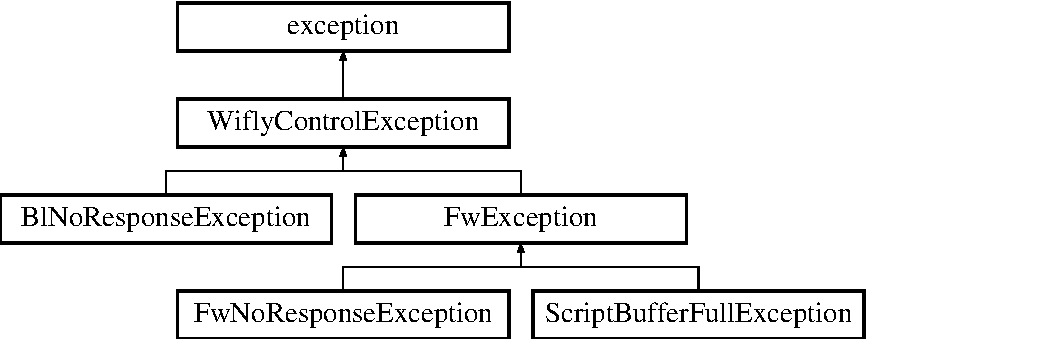
\includegraphics[height=4.000000cm]{class_wifly_control_exception}
\end{center}
\end{figure}
\subsection*{Public Member Functions}
\begin{DoxyCompactItemize}
\item 
\hypertarget{class_wifly_control_exception_a7c12735a818b900b9b5edb6ee5e0e305}{{\bfseries Wifly\-Control\-Exception} (const std\-::string error\-String=\char`\"{}Wifly\-Control\-Exception\char`\"{})}\label{class_wifly_control_exception_a7c12735a818b900b9b5edb6ee5e0e305}

\item 
\hypertarget{class_wifly_control_exception_a0fa2a5e8db72e6927d29c82968319e78}{const char $\ast$ {\bfseries what} (void) const   throw ()}\label{class_wifly_control_exception_a0fa2a5e8db72e6927d29c82968319e78}

\end{DoxyCompactItemize}


\subsection{Detailed Description}
Copyright (C) 2012, 2013 Nils Weiss, Patrick Bruenn.

This file is part of Wifly\-\_\-\-Light.

Wifly\-\_\-\-Light is free software\-: you can redistribute it and/or modify it under the terms of the G\-N\-U General Public License as published by the Free Software Foundation, either version 3 of the License, or (at your option) any later version.

Wifly\-\_\-\-Light is distributed in the hope that it will be useful, but W\-I\-T\-H\-O\-U\-T A\-N\-Y W\-A\-R\-R\-A\-N\-T\-Y; without even the implied warranty of M\-E\-R\-C\-H\-A\-N\-T\-A\-B\-I\-L\-I\-T\-Y or F\-I\-T\-N\-E\-S\-S F\-O\-R A P\-A\-R\-T\-I\-C\-U\-L\-A\-R P\-U\-R\-P\-O\-S\-E. See the G\-N\-U General Public License for more details.

You should have received a copy of the G\-N\-U General Public License along with Wifly\-\_\-\-Light. If not, see \href{http://www.gnu.org/licenses/}{\tt http\-://www.\-gnu.\-org/licenses/}. 

The documentation for this class was generated from the following file\-:\begin{DoxyCompactItemize}
\item 
library/Wifly\-Control\-Exception.\-h\end{DoxyCompactItemize}

\hypertarget{class_wifly_response}{\section{Wifly\-Response Class Reference}
\label{class_wifly_response}\index{Wifly\-Response@{Wifly\-Response}}
}


{\ttfamily \#include $<$Wifly\-Control\-Response.\-h$>$}

Inheritance diagram for Wifly\-Response\-:\begin{figure}[H]
\begin{center}
\leavevmode
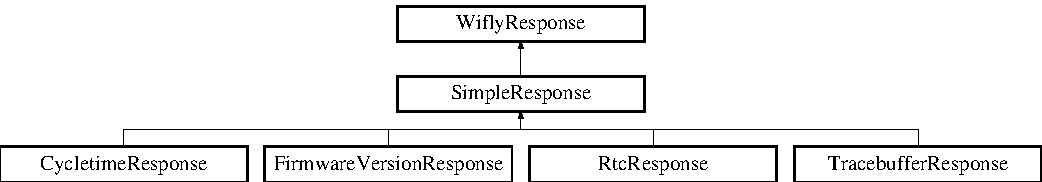
\includegraphics[height=2.441860cm]{class_wifly_response}
\end{center}
\end{figure}
\subsection*{Public Member Functions}
\begin{DoxyCompactItemize}
\item 
\hypertarget{class_wifly_response_aa9df8428eafc9e1cf1bc987aaf18eb79}{virtual void {\bfseries Init} (response\-\_\-frame $\ast$p\-Data, size\-\_\-t data\-Length)=0}\label{class_wifly_response_aa9df8428eafc9e1cf1bc987aaf18eb79}

\item 
\hypertarget{class_wifly_response_a78274601001f1f8e112e1c59ea59f9df}{bool {\bfseries Is\-Valid} (void) const }\label{class_wifly_response_a78274601001f1f8e112e1c59ea59f9df}

\item 
\hypertarget{class_wifly_response_a4b5e58113cf23e0723d0a2d22e0c8acb}{bool {\bfseries Is\-Script\-Buffer\-Full} (void) const }\label{class_wifly_response_a4b5e58113cf23e0723d0a2d22e0c8acb}

\item 
\hypertarget{class_wifly_response_ae28f6e581ab7864969d2bf70b1c44ee0}{bool {\bfseries Is\-Crc\-Check\-Failed} (void) const }\label{class_wifly_response_ae28f6e581ab7864969d2bf70b1c44ee0}

\end{DoxyCompactItemize}
\subsection*{Protected Attributes}
\begin{DoxyCompactItemize}
\item 
\hypertarget{class_wifly_response_a623b14a001d67b20f8b68d4678f980da}{bool {\bfseries m\-Is\-Valid}}\label{class_wifly_response_a623b14a001d67b20f8b68d4678f980da}

\item 
\hypertarget{class_wifly_response_a96140d95b1d54221bf6e81cf723f1192}{bool {\bfseries m\-Is\-Script\-Buffer\-Full}}\label{class_wifly_response_a96140d95b1d54221bf6e81cf723f1192}

\item 
\hypertarget{class_wifly_response_a5e3b9bdb3dea4b9cad2956126b3b18bb}{bool {\bfseries m\-Is\-Crc\-Check\-Failed}}\label{class_wifly_response_a5e3b9bdb3dea4b9cad2956126b3b18bb}

\end{DoxyCompactItemize}


\subsection{Detailed Description}
Copyright (C) 2012, 2013 Nils Weiss, Patrick Bruenn.

This file is part of Wifly\-\_\-\-Light.

Wifly\-\_\-\-Light is free software\-: you can redistribute it and/or modify it under the terms of the G\-N\-U General Public License as published by the Free Software Foundation, either version 3 of the License, or (at your option) any later version.

Wifly\-\_\-\-Light is distributed in the hope that it will be useful, but W\-I\-T\-H\-O\-U\-T A\-N\-Y W\-A\-R\-R\-A\-N\-T\-Y; without even the implied warranty of M\-E\-R\-C\-H\-A\-N\-T\-A\-B\-I\-L\-I\-T\-Y or F\-I\-T\-N\-E\-S\-S F\-O\-R A P\-A\-R\-T\-I\-C\-U\-L\-A\-R P\-U\-R\-P\-O\-S\-E. See the G\-N\-U General Public License for more details.

You should have received a copy of the G\-N\-U General Public License along with Wifly\-\_\-\-Light. If not, see \href{http://www.gnu.org/licenses/}{\tt http\-://www.\-gnu.\-org/licenses/}. 

The documentation for this class was generated from the following file\-:\begin{DoxyCompactItemize}
\item 
library/Wifly\-Control\-Response.\-h\end{DoxyCompactItemize}

\chapter{File Documentation}
\hypertarget{intelhexclass_8cpp}{\section{library/intelhexclass.cpp File Reference}
\label{intelhexclass_8cpp}\index{library/intelhexclass.\-cpp@{library/intelhexclass.\-cpp}}
}
{\ttfamily \#include $<$iostream$>$}\\*
{\ttfamily \#include $<$string$>$}\\*
{\ttfamily \#include $<$vector$>$}\\*
{\ttfamily \#include $<$cstdio$>$}\\*
{\ttfamily \#include \char`\"{}intelhexclass.\-h\char`\"{}}\\*
\subsection*{Enumerations}
\begin{DoxyCompactItemize}
\item 
enum \hyperlink{intelhexclass_8cpp_a3bb353cb1867130c7b77b1e199c66358}{intelhex\-Record\-Type} \{ \\*
{\bfseries D\-A\-T\-A\-\_\-\-R\-E\-C\-O\-R\-D}, 
{\bfseries E\-N\-D\-\_\-\-O\-F\-\_\-\-F\-I\-L\-E\-\_\-\-R\-E\-C\-O\-R\-D}, 
{\bfseries E\-X\-T\-E\-N\-D\-E\-D\-\_\-\-S\-E\-G\-M\-E\-N\-T\-\_\-\-A\-D\-D\-R\-E\-S\-S}, 
{\bfseries S\-T\-A\-R\-T\-\_\-\-S\-E\-G\-M\-E\-N\-T\-\_\-\-A\-D\-D\-R\-E\-S\-S}, 
\\*
{\bfseries E\-X\-T\-E\-N\-D\-E\-D\-\_\-\-L\-I\-N\-E\-A\-R\-\_\-\-A\-D\-D\-R\-E\-S\-S}, 
{\bfseries S\-T\-A\-R\-T\-\_\-\-L\-I\-N\-E\-A\-R\-\_\-\-A\-D\-D\-R\-E\-S\-S}, 
{\bfseries N\-O\-\_\-\-O\-F\-\_\-\-R\-E\-C\-O\-R\-D\-\_\-\-T\-Y\-P\-E\-S}
 \}
\end{DoxyCompactItemize}
\subsection*{Functions}
\begin{DoxyCompactItemize}
\item 
istream \& \hyperlink{intelhexclass_8cpp_a73fb9c5b9d6d069b5eb83340942fd54b}{operator$>$$>$} (istream \&data\-In, \hyperlink{classintelhex}{intelhex} \&ih\-Local)
\item 
ostream \& \hyperlink{intelhexclass_8cpp_a320e23dab311a6c652aa7ddb9e2f9cc2}{operator$<$$<$} (ostream \&data\-Out, \hyperlink{classintelhex}{intelhex} \&ih\-Local)
\end{DoxyCompactItemize}


\subsection{Enumeration Type Documentation}
\hypertarget{intelhexclass_8cpp_a3bb353cb1867130c7b77b1e199c66358}{\index{intelhexclass.\-cpp@{intelhexclass.\-cpp}!intelhex\-Record\-Type@{intelhex\-Record\-Type}}
\index{intelhex\-Record\-Type@{intelhex\-Record\-Type}!intelhexclass.cpp@{intelhexclass.\-cpp}}
\subsubsection[{intelhex\-Record\-Type}]{\setlength{\rightskip}{0pt plus 5cm}enum {\bf intelhex\-Record\-Type}}}\label{intelhexclass_8cpp_a3bb353cb1867130c7b77b1e199c66358}
Possible record types for Intel H\-E\-X file.

List of all possible record types that can be found in an Intel H\-E\-X file. 

\subsection{Function Documentation}
\hypertarget{intelhexclass_8cpp_a320e23dab311a6c652aa7ddb9e2f9cc2}{\index{intelhexclass.\-cpp@{intelhexclass.\-cpp}!operator$<$$<$@{operator$<$$<$}}
\index{operator$<$$<$@{operator$<$$<$}!intelhexclass.cpp@{intelhexclass.\-cpp}}
\subsubsection[{operator$<$$<$}]{\setlength{\rightskip}{0pt plus 5cm}ostream\& operator$<$$<$ (
\begin{DoxyParamCaption}
\item[{ostream \&}]{data\-Out, }
\item[{{\bf intelhex} \&}]{ih\-Local}
\end{DoxyParamCaption}
)}}\label{intelhexclass_8cpp_a320e23dab311a6c652aa7ddb9e2f9cc2}
\begin{DoxyVerb}     Operator overloaded to encode any data held in memory into the Intel
     HEX format for storage on disk                 
\end{DoxyVerb}


\begin{DoxySeeAlso}{See Also}
\hyperlink{intelhexclass_8cpp_a73fb9c5b9d6d069b5eb83340942fd54b}{operator$>$$>$()}
\end{DoxySeeAlso}

\begin{DoxyParams}{Parameters}
{\em data\-Out} & -\/ Output stream for to store the decoded file information \\
\hline
{\em ih\-Local} & -\/ Points to this class so that friend function has access to private class members\\
\hline
\end{DoxyParams}

\begin{DoxyRetVals}{Return values}
{\em -\/} & pointer to output stream \\
\hline
\end{DoxyRetVals}
\hypertarget{intelhexclass_8cpp_a73fb9c5b9d6d069b5eb83340942fd54b}{\index{intelhexclass.\-cpp@{intelhexclass.\-cpp}!operator$>$$>$@{operator$>$$>$}}
\index{operator$>$$>$@{operator$>$$>$}!intelhexclass.cpp@{intelhexclass.\-cpp}}
\subsubsection[{operator$>$$>$}]{\setlength{\rightskip}{0pt plus 5cm}istream\& operator$>$$>$ (
\begin{DoxyParamCaption}
\item[{istream \&}]{data\-In, }
\item[{{\bf intelhex} \&}]{ih\-Local}
\end{DoxyParamCaption}
)}}\label{intelhexclass_8cpp_a73fb9c5b9d6d069b5eb83340942fd54b}
\begin{DoxyVerb}     Operator overloaded to decode data streamed in from a file in the 
     Intel HEX format into memory                 
\end{DoxyVerb}


\begin{DoxySeeAlso}{See Also}
\hyperlink{intelhexclass_8cpp_a320e23dab311a6c652aa7ddb9e2f9cc2}{operator$<$$<$()}
\end{DoxySeeAlso}

\begin{DoxyParams}{Parameters}
{\em data\-In} & -\/ Input stream for the encoded file information \\
\hline
{\em ih\-Local} & -\/ Points to this class so that friend function has access to private class members\\
\hline
\end{DoxyParams}

\begin{DoxyRetVals}{Return values}
{\em -\/} & pointer to input stream \\
\hline
\end{DoxyRetVals}

\hypertarget{intelhexclass_8h}{\section{library/intelhexclass.h File Reference}
\label{intelhexclass_8h}\index{library/intelhexclass.\-h@{library/intelhexclass.\-h}}
}
{\ttfamily \#include $<$iostream$>$}\\*
{\ttfamily \#include $<$map$>$}\\*
{\ttfamily \#include $<$list$>$}\\*
\subsection*{Classes}
\begin{DoxyCompactItemize}
\item 
class \hyperlink{classintelhex}{intelhex}
\begin{DoxyCompactList}\small\item\em Class to decode, encode and manipulate Intel H\-E\-X format files. \end{DoxyCompactList}\end{DoxyCompactItemize}


\subsection{Detailed Description}
\begin{DoxyAuthor}{Author}
Stuart Cording aka C\-O\-D\-I\-N\-G\-H\-E\-A\-D
\end{DoxyAuthor}
A class to handle the encoding, decoding and manipulatio of an Intel H\-E\-X format file as generated by many tool chains for embedded processors and microcontrollers.

This class is constructed based upon the definition given in the document 'Hexadecimal Object File Format Specification', Revision A, January 6, 1988, © 1998 Intel Corporation.

\begin{DoxyNote}{Note}
See the git versioning notes for version information 
\end{DoxyNote}

\addcontentsline{toc}{part}{Index}
\printindex
\end{document}
